%%% ---  TEMPLATE PARA ELABORAÇÃO DO TRABALHO DE CONCLUSÃO DE CURSO
% DO CURSO DE ESTATÍSTICA DA UFSCar

\documentclass[12pt,twoside]{book} 
\usepackage[utf8]{inputenc}
\usepackage[T1]{fontenc}
\usepackage{lmodern}
\usepackage[brazil]{babel}\pdfmapfile{+pdftex.map}
\usepackage{amsmath, amsfonts, amssymb}
\usepackage{mathrsfs}
\usepackage{graphicx}      			% Inclusão de gráficos
\usepackage{tikz}
\usetikzlibrary{arrows.meta,positioning,fit}
\graphicspath{{figuras/}{../figuras/}}
\usepackage{flafter}
\usepackage{float}                  % Controle rígido de floats
\usepackage{microtype}
\usepackage{longtable}
\usepackage{geometry, calc, setspace}
\usepackage[table]{xcolor}
\usepackage{indentfirst}
\usepackage[round]{natbib}
\usepackage{booktabs}
\usepackage[hyphens]{url}
\usepackage{array}
\usepackage{tabularx}
\usepackage{multirow}

% Tabelas: fonte, espaçamento e largura padronizados
\newcolumntype{Y}{>{\raggedright\arraybackslash}X}
\newcommand{\thesistablesetup}{%
  \small
  \setlength{\tabcolsep}{6pt}%
  \renewcommand{\arraystretch}{1.12}%
}
% Rótulos legíveis de covariáveis (glossário, Tabela~\ref{tab:variaveis})
\newcommand{\vGamesMissed}{Jogos perdidos}
\newcommand{\vDepthTeam}{Profundidade no elenco}
\newcommand{\vOffensePct}{Participação ofensiva}
\newcommand{\vPasserRating}{Eficiência de passe}
\newcommand{\vTeamPassShare}{Fatia de passes}
\newcommand{\vTeamTargetsShare}{Fatia de alvos}
\newcommand{\vTeamRushShare}{Fatia de jardas terrestres}
\newcommand{\vPreVeteran}{Veterano pré-janela}
\newcommand{\vUndrafted}{Não draftado}
\newcommand{\vDraftOvr}{Posição no \textit{draft}}
\newcommand{\vGapYears}{Hiato acumulado}
\newcommand{\vUnobsHist}{Histórico pré-janela não observado}
\newcommand{\vLagTdPct}{Hist. defasado TD\%}
\newcommand{\vLagYpc}{Hist. defasado YPC}
\newcommand{\vLagFumble}{Hist. defasado fumbles perdidos}
\newcommand{\vLagRushYds}{Hist. defasado jardas de corrida}
\newcommand{\vHeight}{Altura}
\newcommand{\vLagCatchRate}{Hist. defasado taxa de recepção}
\newcommand{\vPreExp}{Experiência pré-janela}
\newcommand{\vLagCompMiss}{Hist. defasado comp\% (ausente)}
\newcommand{\vLagRedzone}{Hist. defasado alvos na \textit{red zone}}
\newcommand{\vAge}{Idade}
\usepackage{needspace}
\usepackage[section,above]{placeins}
\usepackage{caption}
\usepackage{hyperref} \hypersetup{colorlinks, citecolor=blue, filecolor=red, linkcolor=blue, urlcolor=blue}

% Reduz espaçamento entre figuras/tabelas e texto
\setlength{\textfloatsep}{8pt plus 2pt minus 2pt}
\setlength{\intextsep}{8pt plus 2pt minus 2pt}
\setlength{\floatsep}{6pt plus 2pt minus 2pt}
\setlength{\abovecaptionskip}{4pt}
\setlength{\belowcaptionskip}{2pt}

% Permite que o LaTeX preencha mais da página com figuras
\renewcommand{\topfraction}{0.92}
\renewcommand{\bottomfraction}{0.92}
\renewcommand{\textfraction}{0.08}
\renewcommand{\floatpagefraction}{0.85}

% Reduz overfull hbox em parágrafos justificados
\emergencystretch=1em

\def\us{\char`\_}       % inserir underline no texto.  

% Figuras calibradas: largura = \textwidth, sem height cap
\newcommand{\thesisfig}[1]{\includegraphics[width=\textwidth,height=0.60\textheight,keepaspectratio]{#1}}
\newcommand{\thesisfigwide}[1]{\includegraphics[width=\textwidth,height=0.22\textheight,keepaspectratio]{#1}}
\newcommand{\thesisfigforestfull}[1]{\includegraphics[width=\textwidth,height=0.28\textheight,keepaspectratio]{#1}}
\newcommand{\thesisfigforestcompact}[1]{\includegraphics[width=\textwidth,height=0.19\textheight,keepaspectratio]{#1}}
\newcommand{\thesisfigfit}[1]{\includegraphics[width=\textwidth,height=0.36\textheight,keepaspectratio]{#1}}
\newcommand{\thesisfigkm}[1]{\includegraphics[width=\textwidth,height=0.28\textheight,keepaspectratio]{#1}}
\newcommand{\thesisfigfitfill}[1]{\includegraphics[width=\textwidth,height=0.40\textheight,keepaspectratio]{#1}}
\newcommand{\thesisfigfitpair}[1]{\includegraphics[width=\textwidth,height=0.35\textheight,keepaspectratio]{#1}}
\newcommand{\thesisfigdraft}[1]{\thesisfigwide{#1}}
\newcommand{\thesisfigdrafttrio}[1]{\includegraphics[width=\textwidth,height=0.28\textheight,keepaspectratio]{#1}}
\newcommand{\thesisfigdraftfill}[1]{\includegraphics[width=\textwidth,height=0.35\textheight,keepaspectratio]{#1}}
\newcommand{\thesisfigdraftpair}[1]{\includegraphics[width=\textwidth,height=0.41\textheight,keepaspectratio]{#1}}
\newcommand{\thesisfigcompact}[1]{\includegraphics[width=\textwidth,height=0.30\textheight,keepaspectratio]{#1}}
\newcommand{\thesisfigcompacttrio}[1]{\includegraphics[width=\textwidth,height=0.29\textheight,keepaspectratio]{#1}}
\newcommand{\thesisfigaalenpar}[1]{\includegraphics[width=\textwidth,height=0.22\textheight,keepaspectratio]{#1}}
\newcommand{\thesisfigsolo}[1]{\includegraphics[width=\textwidth,height=0.60\textheight,keepaspectratio]{#1}}
\newcommand{\thesisfigtall}[1]{\includegraphics[width=\textwidth,height=0.60\textheight,keepaspectratio]{#1}}
\newcommand{\thesisfigaalen}[1]{\includegraphics[width=\textwidth,height=0.68\textheight,keepaspectratio]{#1}}
\newcommand{\thesisfigaalenq}[1]{\includegraphics[width=\textwidth,height=0.78\textheight,keepaspectratio]{#1}}
\newcommand{\thesisfigaalenpack}[1]{\includegraphics[width=\textwidth,height=0.70\textheight,keepaspectratio]{#1}}
\newcommand{\thesisfigaalenwr}[1]{\includegraphics[width=\textwidth,height=0.65\textheight,keepaspectratio]{#1}}
\newcommand{\thesisfigaalenpage}[1]{\includegraphics[width=\textwidth,height=0.82\textheight,keepaspectratio]{#1}}
\newcommand{\paneltag}[1]{%
  \par\vspace{0.15em}%
  \noindent\textbf{(#1)}%
  \par\vspace{0.08em}%
}
\newcommand{\paneltagpad}[1]{%
  \par\vspace{0.25em}%
  \noindent\textbf{(#1)}%
  \par\vspace{0.85em}%
}
\newcommand{\thesisfigpanel}[3]{%
  \paneltag{#1}%
  #2{#3}%
}
\newcommand{\thesisfigcareerlag}{%
  \includegraphics[width=\textwidth,height=0.70\textheight,keepaspectratio]{figuras/career_lag_evo_QB.pdf}%
}
\newcommand{\thesisfigcareerlagtop}{%
  \includegraphics[width=\textwidth,height=0.48\textheight,clip,trim=0 295.4pt 0 0,keepaspectratio]{figuras/career_lag_evo_QB.pdf}%
}
\newcommand{\thesisfigcareerlagbot}{%
  \includegraphics[width=\textwidth,height=0.36\textheight,clip,trim=0 0 0 295.4pt,keepaspectratio]{figuras/career_lag_evo_QB.pdf}%
}
% Schoenfeld / forest: caixa fixa para pares com alturas nativas distintas
\newcommand{\thesisfigschoen}[1]{\includegraphics[width=\textwidth,height=0.34\textheight,keepaspectratio]{#1}}
\newcommand{\thesisfigschoenqb}[1]{\includegraphics[width=\textwidth,height=0.36\textheight,keepaspectratio]{#1}}
\newcommand{\thesisfigschoenpanel}[1]{\includegraphics[width=\textwidth,height=0.39\textheight,keepaspectratio]{#1}}
\newcommand{\thesisschoenpair}[4]{%
  \begin{figure}[H]
  \centering
  \thesisfigschoen{#1}
  \captionof{figure}{#2}
  \vspace{0.25em}
  \thesisfigschoen{#3}
  \captionof{figure}{#4}
  \end{figure}%
}
\newcommand{\thesisfigcomp}[1]{\includegraphics[width=\textwidth,height=0.62\textheight,keepaspectratio]{#1}}
\newcommand{\thesisfigforest}[1]{\includegraphics[width=\textwidth,height=0.20\textheight,keepaspectratio]{#1}}
\newcommand{\thesisforestpair}[5]{%
  \begin{figure}[H]
  \centering
  \thesisfigforest{#1}
  \captionof{figure}{#2}
  \vspace{0.1em}
  \thesisfigforest{#3}
  \captionof{figure}{#4}
  \label{#5}
  \end{figure}%
}
% Mantém parágrafo + figura QB juntos (evita figura órfã na página seguinte)
\newcommand{\thesiskeep}[1]{\par\needspace{#1}}
\newcommand{\thesiskeepfig}[1]{\thesiskeep{#1}}
% Trio comparativo: 1ª figura sob o parágrafo; par RB+WR na página seguinte
\newcommand{\thesisone}[2]{%
  \begin{figure}[H]
  \centering
  \thesisfig{#1}
  \caption{#2}
  \end{figure}%
}
\newcommand{\thesisonekm}[2]{%
  \begin{figure}[H]
  \centering
  \thesisfig{#1}
  \caption{#2}
  \end{figure}%
}
\newcommand{\thesisonefit}[2]{%
  \begin{figure}[H]
  \centering
  \thesisfigsolo{#1}
  \caption{#2}
  \end{figure}%
}
\newcommand{\thesispair}[4]{%
  \begin{figure}[H]
  \centering
  \thesisfig{#1}
  \captionof{figure}{#2}
  \vspace{0.35em}
  \thesisfig{#3}
  \captionof{figure}{#4}
  \end{figure}%
}
\newcommand{\thesispairfit}[4]{%
  \begin{figure}[H]
  \centering
  \thesisfigfit{#1}
  \captionof{figure}{#2}
  \vspace{0.3em}
  \thesisfigfit{#3}
  \captionof{figure}{#4}
  \end{figure}%
}
% Figura fit inline (flui após parágrafo, sem float único — evita página vazia)
\newcommand{\thesisonefitinline}[2]{%
  \thesisonefit{#1}{#2}%
}
\newcommand{\thesispairfitinline}[4]{%
  \thesispairfit{#1}{#2}{#3}{#4}%
}
\newcommand{\thesispairdraftinline}[4]{%
  \begin{figure}[htbp]
  \centering
  \includegraphics[width=\textwidth,height=0.34\textheight,keepaspectratio]{#1}
  \captionof{figure}{#2}
  \medskip
  \includegraphics[width=\textwidth,height=0.34\textheight,keepaspectratio]{#3}
  \captionof{figure}{#4}
  \end{figure}%
}
% Par compacto inline (2 figuras na mesma página do parágrafo, ex.: dist_carreira)
\newcommand{\thesispaircompact}[4]{%
  \begin{figure}[htbp]
  \centering
  \includegraphics[width=\textwidth,height=0.3\textheight,keepaspectratio]{#1}
  \captionof{figure}{#2}
  \medskip
  \includegraphics[width=\textwidth,height=0.3\textheight,keepaspectratio]{#3}
  \captionof{figure}{#4}
  \end{figure}%
}
\newcommand{\thesispairlabeled}[5]{%
  \begin{figure}[H]
  \centering
  \thesisfig{#1}
  \captionof{figure}{#2}
  \vspace{0.35em}
  \thesisfig{#3}
  \captionof{figure}{#4}
  \label{#5}
  \end{figure}%
}
\newcommand{\thesispairfitlabeled}[5]{%
  \begin{figure}[H]
  \centering
  \thesisfigfit{#1}
  \captionof{figure}{#2}
  \vspace{0.3em}
  \thesisfigfit{#3}
  \captionof{figure}{#4}
  \label{#5}
  \end{figure}%
}
\newcommand{\thesisstack}[3]{%
  \thesisfig{#1}\\[0.35em]
  \thesisfig{#2}\\[0.35em]
  \thesisfig{#3}%
}
\newcommand{\figtriocite}[3]{Figuras~\ref{#1}, \ref{#2} e~\ref{#3}}
\newcommand{\figtrio}[1]{Figura~\ref{#1}}
\newcommand{\thesispaircompactlabeled}[6]{%
  \begin{figure}[htbp]
  \centering
  \includegraphics[width=\textwidth,height=0.3\textheight,keepaspectratio]{#1}
  \captionof{figure}{#2}\label{#3}
  \medskip
  \includegraphics[width=\textwidth,height=0.3\textheight,keepaspectratio]{#4}
  \captionof{figure}{#5}\label{#6}
  \end{figure}%
}
\newcommand{\thesispairdraftlabeled}[6]{%
  \begin{figure}[htbp]
  \centering
  \includegraphics[width=\textwidth,height=0.34\textheight,keepaspectratio]{#1}
  \captionof{figure}{#2}\label{#3}
  \medskip
  \includegraphics[width=\textwidth,height=0.34\textheight,keepaspectratio]{#4}
  \captionof{figure}{#5}\label{#6}
  \end{figure}%
}
\newcommand{\thesistriodraftlabeled}[9]{%
  \begin{figure}[p]
  \centering
  \includegraphics[width=\textwidth,height=0.25\textheight,keepaspectratio]{#1}
  \captionof{figure}{#2}\label{#3}
  \medskip
  \includegraphics[width=\textwidth,height=0.25\textheight,keepaspectratio]{#4}
  \captionof{figure}{#5}\label{#6}
  \medskip
  \includegraphics[width=\textwidth,height=0.25\textheight,keepaspectratio]{#7}
  \captionof{figure}{#8}\label{#9}
  \end{figure}%
}
\newcommand{\thesisonedraftinlinelabeled}[3]{%
  \begin{figure}[htbp]
  \centering
  \includegraphics[width=\textwidth,height=0.5\textheight,keepaspectratio]{#1}
  \caption{#2}\label{#3}
  \end{figure}%
}
\newcommand{\thesispairdraftpagelabeled}[6]{%
  \begin{figure}[htbp]
  \centering
  \includegraphics[width=\textwidth,height=0.34\textheight,keepaspectratio]{#1}
  \captionof{figure}{#2}\label{#3}
  \medskip
  \includegraphics[width=\textwidth,height=0.34\textheight,keepaspectratio]{#4}
  \captionof{figure}{#5}\label{#6}
  \end{figure}%
}
\newcommand{\thesisonefitinlinelabeled}[3]{%
  \begin{figure}[htbp]
  \centering
  \includegraphics[width=\textwidth,height=0.5\textheight,keepaspectratio]{#1}
  \caption{#2}\label{#3}
  \end{figure}%
}
\newcommand{\thesispairfitpagelabeled}[6]{%
  \begin{figure}[htbp]
  \centering
  \includegraphics[width=\textwidth,height=0.35\textheight,keepaspectratio]{#1}
  \captionof{figure}{#2}\label{#3}
  \medskip
  \includegraphics[width=\textwidth,height=0.35\textheight,keepaspectratio]{#4}
  \captionof{figure}{#5}\label{#6}
  \end{figure}%
}
\newcommand{\thesistriocompactlabeled}[9]{%
  \begin{figure}[p]
  \centering
  \includegraphics[width=\textwidth,height=0.25\textheight,keepaspectratio]{#1}
  \captionof{figure}{#2}\label{#3}
  \medskip
  \includegraphics[width=\textwidth,height=0.25\textheight,keepaspectratio]{#4}
  \captionof{figure}{#5}\label{#6}
  \medskip
  \includegraphics[width=\textwidth,height=0.25\textheight,keepaspectratio]{#7}
  \captionof{figure}{#8}\label{#9}
  \end{figure}%
}
\newcommand{\thesispairfitlabeledtwo}[6]{%
  \begin{figure}[H]
  \centering
  \thesisfigfit{#1}
  \captionof{figure}{#2}
  \label{#3}
  \vspace{0.3em}
  \thesisfigfit{#4}
  \captionof{figure}{#5}
  \label{#6}
  \end{figure}%
}
\newcommand{\thesisonecompactlabeled}[3]{%
  \begin{figure}[H]
  \centering
  \thesisfigcompact{#1}
  \caption{#2}
  \label{#3}
  \end{figure}%
}
\newcommand{\thesisonedraftlabeled}[3]{%
  \begin{figure}[H]
  \centering
  \thesisfigsolo{#1}
  \caption{#2}
  \label{#3}
  \end{figure}%
}
\newcommand{\thesisonefitlabeled}[3]{%
  \begin{figure}[H]
  \centering
  \thesisfigsolo{#1}
  \caption{#2}
  \label{#3}
  \end{figure}%
}
\newcommand{\thesisonefitwrlabeled}[3]{%
  \begin{figure}[H]
  \centering
  \thesisfigfit{#1}
  \caption{#2}
  \label{#3}
  \end{figure}%
}

\geometry{a4paper, headsep=1.0cm, footskip=1cm, lmargin=3cm, rmargin=2cm, tmargin=2.5cm, bmargin=2cm, headheight=2.5cm}

% Evita páginas em branco entre capítulos e elementos pré-textuais
\let\origcleardoublepage\cleardoublepage % página em branco só nos elementos pré-textuais
\let\cleardoublepage\clearpage

% Remove espaço vertical excessivo antes dos títulos de capítulos e listas
\makeatletter
\def\@makechapterhead#1{%
  \vspace*{0pt}
  {\parindent \z@ \raggedright \normalfont
    \ifnum \c@secnumdepth >\m@ne
      \if@mainmatter
        \huge\bfseries \@chapapp\space \thechapter
        \par\nobreak
        \vskip 20\p@
      \fi
    \fi
    \interlinepenalty\@M
    \Huge \bfseries #1\par\nobreak
    \vskip 20\p@
  }}
\def\@makeschapterhead#1{%
  \vspace*{0pt}
  {\parindent \z@ \raggedright
    \normalfont
    \interlinepenalty\@M
    \Huge \bfseries  #1\par\nobreak
    \vskip 20\p@
  }}
\makeatother

%%%%%%%%%%%%%%%%%%%%%%%%%%%%%%%%%%%%%%%%%%%%%%%%%%%%%%%%%%%%
\usepackage{theorem}
%\theorembodyfont{\normalfont\upshape} %  fonte normal para teoremas

\numberwithin{equation}{chapter} % usar contador associado ao capítulo
\newtheorem{teo}[equation]{Teorema} 
\newtheorem{axi}[equation]{Axioma}
\newtheorem{defn}[equation]{Definição}
\newtheorem{result}[equation]{Resultado}
\newtheorem{propdd}[equation]{Propriedades}
\newtheorem{obs}[equation]{Observação}
\newtheorem{exerc}[equation]{Exercício}
\newtheorem{explo}[equation]{Exemplo}
\newtheorem{aplic}[equation]{Aplicações}
\newenvironment{proof}[1][Proof]{\textbf{#1.} }{\ \rule{0.5em}{0.5em}}

\newcommand*{\nomemes}{\ifcase\month\or Janeiro\or Fevereiro\or Mar\c{c}o\or
                       Abril\or Maio\or Junho\or Julho\or Agosto\or Setembro\or
                       Outubro\or Novembro\or Dezembro \fi}
\newcommand*{\nomemesEN}{\ifcase\month\or January\or February\or March\or
                       April\or May\or June\or July\or August\or September\or
                       October\or November\or December \fi}

\renewcommand{\baselinestretch}{1.4}  % Espaço entre linhas
\raggedbottom  % Evita espaços verticais esticados entre floats
\widowpenalty=9999       % Penaliza viúvas (linha isolada no topo da página)
\clubpenalty=9999        % Penaliza orfãs (linha isolada no fim da página)
\displaywidowpenalty=9999

%%% --- Início do documento ---%%%
\begin{document}

%%% --- Inclusão de gráficos e figuras ---%%%
\DeclareGraphicsExtensions{.jpg,.pdf,.mps,.png}      

%%% --- ELEMENTOS PRÉ-TEXTUAIS --- %%%
\pagestyle{empty}

%%% --- Inclusão da capa --- %%%
%%% --- CAPA --- %%%
\thispagestyle{empty} 


%%% --- Nome da Instituição --- %%%
\begin{center}
{\large \bf \sc Universidade Federal de São Carlos \\
Centro de Ciências Exatas e de Tecnologia \\
Departamento de Estatística} \\
\end{center}
\vspace*{6cm}

%%% --- Título do Trabalho --- %%%
\begin{center}
{\Large{\bf  Sobrevivência na NFL: Análise e Predição de \\
Longevidade de Carreira entre QBs, WRs e RBs}}
\end{center}
\vspace*{2cm}

%%% --- Nome da(o) aluna(o) --- %%%
\begin{center} 
 {\large \bf Arthur Pereira Gon} 
\end{center}
\vspace*{7.8cm}

%%% --- TCC --- %%%
\begin{center} 
{\large \bf Trabalho de Conclusão de Curso} 
\end{center}
\setcounter{page}{0}

%%% --- Inclusão da folha de rosto 1 --- %%%
%%% --- FOLHA DE ROSTO 1 --- %%%
% ATENÇÃO: 
% Esta página deve ser inserida na versão entregue à
% banca examinadora tanto no TG1 quanto no TG2


\clearpage{\thispagestyle{empty}\origcleardoublepage}
\thispagestyle{empty}
\begin{center}
{\large \sc Universidade Federal de São Carlos \\
Centro de Ciências Exatas e de Tecnologia \\
Departamento de Estatística} \\
\end{center}

\vspace*{2cm}

%%% --- Título do Trabalho --- %%%
\begin{center}
{\Large Sobrevivência na NFL: Análise e Predição de \\
Longevidade de Carreira entre QBs, WRs e RBs}
\end{center}
\vspace{2.5cm}

%%% --- Nome do(a) aluno(a) e orientador(a) --- %%%
\begin{center}
{\bf {\large Arthur Pereira Gon} \\ 
Orientador: Victor Azevedo Coscrato}
\end{center}
\vspace*{3cm}

%%% --- Texto padrão da obtenção do grau --- %%% 
\begin{flushright}
\begin{minipage}{0.55\textwidth}
Trabalho de Conclusão de Curso apresentado como parte dos requisitos para obtenção do título de Bacharel em Estatística.\\ 
\end{minipage}
\end{flushright}
\vspace{2cm}

%%% --- Local e Data --- %%%
\begin{center} 
{\bf São Carlos\\
Novembro de 2026}
\end{center}

   

%%% --- Inclusão da folha de rosto 2 --- %%%
%%% --- FOLHA DE ROSTO 2 --- %%%
% ATENÇÃO: 
% Esta página deve ser inserida na VERSÃO FINAL do trabalho, 
% após as correções propostas pela banca examinadora, antes
% do depósito no Repositório Institucional da UFSCar.

\clearpage{\thispagestyle{empty}\origcleardoublepage}
\thispagestyle{empty}
\begin{center}
{\large \sc Federal University of São Carlos \\
Exact and Technology Sciences Center \\
Department of Statistics} \\
\end{center}

\vspace*{2cm}

%%% --- Título do Trabalho --- %%%
\begin{center}
{\Large Survival in the NFL: Analysis and Prediction of \\
Career Longevity among QBs, WRs and RBs}
\end{center}
\vspace{2.5cm}

%%% --- Nome do(a) aluno(a) e orientador(a) --- %%%
\begin{center}
{\bf {\large Arthur Pereira Gon} \\ 
Advisor: Victor Azevedo Coscrato}
\end{center}
\vspace*{3cm}

%%% --- Texto padrão da obtenção do grau --- %%% 
\begin{flushright}
\begin{minipage}{0.55\textwidth}
Bachelor's dissertation submitted to the Department of Statistics,  Federal University of São Carlos - DEs-UFSCar, in partial fulfillment of the requirements for the degree of Bachelor in Statistics.\\ 
\end{minipage}
\end{flushright}
\vspace{2cm}

%%% --- Local e Data --- %%%
\begin{center} 
{\bf São Carlos\\
November 2026}
\end{center}   
% incluir somente para o depósito, após incluir as correções propostas pela banca

%%% --- Inclusão da folha de rosto 3 --- %%%
%%% --- FOLHA DE ROSTO 3 --- %%%
% ATENÇÃO:
% Página com título e banca examinadora do trabalho APROVADO.
% Inserir esta página apenas na VERSÃO FINAL do trabalho,
% após as correções propostas pela banca examinadora, antes
% do depósito no Repositório Institucional da UFSCar.

\clearpage{\thispagestyle{empty}\origcleardoublepage}
\thispagestyle{empty}

%%% --- Nome do(a) aluno(a) e do título do TCC --- %%%
\begin{center}
{\Large Arthur Pereira Gon} \\
\vspace{4cm}
{\Large Sobrevivência na NFL: Análise e Predição de \\
Longevidade de Carreira entre QBs, WRs e RBs}
\end{center}
\vspace{4.5cm}

%%% --- Texto padrão da obtenção do grau --- %%% 
\begin{flushright}
\begin{minipage}{0.55\textwidth}
Este exemplar corresponde à redação final do TCC defendido por Arthur Pereira Gon e apresentado em novembro de 2026.
\end{minipage}
\end{flushright}
\vspace{4.5cm}

%%% --- Banca examinadora --- %%% 
Banca Examinadora:
\begin{itemize}
	\item Prof. Dr. Victor Azevedo Coscrato (Orientador)
	\item Profa. Dra. Teresa Cristina Martins Dias
	\item Prof. Dr. Renato Jacob Gava
\end{itemize}  
% incluir somente para o depósito, após incluir as correções propostas pela banca

%%% --- Dedicatória --- %%%
%%% --- DEDICATÓRIA --- %%%
\clearpage{\thispagestyle{empty}\origcleardoublepage}
\thispagestyle{empty}
\vspace*{10cm}

\begin{spacing}{1.65}
\begin{center}
\itshape
Dedico este trabalho aos meus pais, Ana Cláudia e Júlio, e à minha irmã, Thaina, que tornaram este sonho possível e me deram apoio, carinho e amor em cada passo desta caminhada. Dedico também à minha namorada, Carolina, e aos familiares e amigos que estiveram sempre ao meu lado.
\end{center}
\end{spacing}

% incluir somente para o depósito, após incluir as correções propostas pela banca (opcional)

%%% --- Agradecimentos --- %%%
%%% --- AGRADECIMENTOS --- %%%
\clearpage{\thispagestyle{empty}\origcleardoublepage}
\thispagestyle{empty}
\vspace*{1cm}

\begin{center}
{\LARGE Agradecimentos}
\end{center}
\vspace*{1.6cm}

\begin{spacing}{1.65}
Chegar até aqui não foi um caminho solitário, e tenho muito a agradecer. Aos meus pais e à minha irmã, pelo apoio, pelo incentivo e por sempre acreditarem no meu sonho. Aos meus cachorros, Costelinha e Tobias, e à minha gata, Midnight, pelo carinho de todos os dias.

Ao meu orientador, Victor Coscrato, pela orientação, pela paciência e por tudo o que aprendi com ele ao longo deste trabalho. À UFSCar e ao Departamento de Estatística, pelo curso, pela estrutura e por tudo o que me proporcionaram durante a graduação.

Aos meus amigos Ariel, Isabella e Murilo, pela parceria desde o começo da faculdade e por todas as memórias que criamos nesses anos.

E, por fim, mas não menos importante, à minha namorada, Carolina, pelo carinho, pelo apoio e pela motivação em cada etapa desta trajetória. Ter você ao meu lado deixou tudo mais leve.
\end{spacing}

% incluir somente para o depósito, após incluir as correções propostas pela banca (opcional)

%%% --- Epígrafe --- %%%
% %%% --- EPÍGRAFE --- %%%
% ATENÇÃO:
% A epígrafe é opcional.
% Inserir esta página apenas na VERSÃO FINAL do trabalho,
% após as correções propostas pela banca examinadora, antes
% do depósito no Repositório Institucional da UFSCar.

\clearpage{\thispagestyle{empty}\cleardoublepage}
\thispagestyle{empty}
\vspace*{20cm}

\begin{flushright}
{\it Inserir aqui a epígrafe. Exemplo: \\
``Só os loucos sabem.''}\\
(Charlie Brown)
\end{flushright}
% incluir somente para o depósito, após incluir as correções propostas pela banca (opcional)

%%% --- Resumo --- %%%
\clearpage{\thispagestyle{empty}\origcleardoublepage}
\thispagestyle{empty}
\begin{center}
{\LARGE Resumo}
\end{center}
\medskip

Este trabalho estuda quanto tempo dura a carreira de \textit{quarterbacks} (QB), \textit{running backs} (RB) e \textit{wide receivers} (WR) na \textit{National Football League}, nas temporadas de 2012 a 2024, e quais características de uma temporada acompanham a saída da liga. Os dados formam um painel anual por jogador e temporada, em que a saída é a última temporada do jogador na liga, com covariáveis de desempenho, uso, papel na equipe, disponibilidade e histórico de carreira defasado até a temporada anterior.

Na inferência, o modelo de Cox com covariáveis dependentes do tempo estima o efeito médio de cada covariável, e os modelos aditivo de Aalen e híbrido de Cox--Aalen mostram como esse efeito se acumula ao longo da carreira. Na predição, o Cox penalizado, o \textit{Gradient Boosting Survival Analysis} (GBSA) e as \textit{Random Survival Forests} (RSF) são comparados ao Kaplan--Meier por validação \textit{walk-forward} de 2018 a 2021, com hiperparâmetros escolhidos apenas no treino, sobre um conjunto de 21 a 25 covariáveis por posição. A métrica principal é o índice de concordância de Harrell ($C$).

A eficiência de passe é o sinal mais estável do QB, com razão de riscos de $0{,}65$ por desvio-padrão. Os jogos perdidos se associam a maior risco de saída no RB e no WR, e cada desvio-padrão, cerca de cinco jogos, soma em média cerca de 0,1 ao risco de cada ano no meio da carreira. A fatia de alvos da equipe tem a maior magnitude no WR, com razão de riscos de $0{,}27$ por desvio-padrão. Na predição, os modelos com covariáveis ordenam os jogadores bem acima do acaso, com $C$ entre $0{,}66$ e $0{,}71$, contra $0{,}56$ a $0{,}62$ de um Cox só com a experiência. No quintil de maior risco, 45\% dos QBs, 52\% dos RBs e 50\% dos WRs não voltam na temporada seguinte, contra nenhum QB, 1\% dos RBs e 2\% dos WRs no de menor risco.

Para avaliar elencos, as ausências e o papel do jogador na equipe servem de sinais a acompanhar a cada temporada. Em anos, o erro absoluto médio fica entre $1{,}27$ e $1{,}40$, contra $1{,}41$ a $1{,}52$ do Kaplan--Meier, e 37\% a 53\% das previsões erram por até um ano, contra 35\% a 39\%. Como de 47\% a 63\% das previsões erram por mais de um ano, o modelo serve mais para ordenar jogadores que para fixar um prazo.

\medskip
\noindent\textbf{Palavras-chave}: análise de sobrevivência, covariáveis dependentes do tempo, modelo aditivo de Aalen, modelo de Cox, predição de sobrevivência, \textit{National Football League}.


%%% --- Abstract --- %%%
\clearpage{\thispagestyle{empty}\origcleardoublepage}
\thispagestyle{empty}
\begin{center}
{\LARGE Abstract}
\end{center}
\medskip

This study examines how long careers last for quarterbacks (QB), running backs (RB), and wide receivers (WR) in the National Football League, across the 2012 to 2024 seasons, and which characteristics of a season accompany leaving the league. The data form an annual panel of players and seasons, in which departure is a player's last season in the league, with covariates measuring performance, usage, team role, availability and lagged career history up to the previous season.

In the inferential analysis, a Cox model with time-dependent covariates estimates the average effect of each covariate, and the Aalen additive model and the hybrid Cox--Aalen model show how this effect accumulates over the career. In the predictive analysis, penalized Cox, Gradient Boosting Survival Analysis (GBSA) and Random Survival Forests (RSF) are compared with Kaplan--Meier through walk-forward validation from 2018 to 2021, with hyperparameters chosen only on the training data, over a set of 21 to 25 covariates per position. The main metric is Harrell's concordance index ($C$).

Passing efficiency is the most stable signal for QBs, with a hazard ratio of $0.65$ per standard deviation. Games missed are associated with a higher risk of leaving among RBs and WRs, and each standard deviation, about five games, adds on average about 0.1 to the risk of each mid-career year. The fraction of team targets has the largest magnitude among WRs, with a hazard ratio of $0.27$ per standard deviation. In prediction, the models with covariates rank players well above chance, with $C$ between $0.66$ and $0.71$, against $0.56$ to $0.62$ for a Cox model with experience only. In the highest-risk quintile, 45\% of QBs, 52\% of RBs and 50\% of WRs do not return the next season, against no QB, 1\% of RBs and 2\% of WRs in the lowest-risk quintile.

For roster evaluation, absences and a player's role on the team serve as signals to monitor from season to season. In years, the mean absolute error lies between $1.27$ and $1.40$, against $1.41$ to $1.52$ for Kaplan--Meier, and 37\% to 53\% of the predictions are off by at most one year, against 35\% to 39\%. Since 47\% to 63\% of the predictions miss by more than one year, the model serves better to rank players than to set a deadline.

\medskip
\noindent\textbf{Keywords}: survival analysis, time-dependent covariates, Aalen additive model, Cox model, survival prediction, National Football League.

% incluir somente para o depósito, após incluir as correções propostas pela banca


%%% --- Lista de figuras --- %%%
\clearpage{\thispagestyle{empty}\origcleardoublepage}
\listoffigures
\thispagestyle{empty}
\clearpage{\thispagestyle{empty}\origcleardoublepage}
% opcional

%%% --- Lista de tabelas --- %%%
\clearpage{\thispagestyle{empty}\origcleardoublepage}
\listoftables
\thispagestyle{empty}
\clearpage{\thispagestyle{empty}\origcleardoublepage}
%opcional

%%% --- Sumário --- %%%
\setcounter{tocdepth}{1}
\clearpage{\thispagestyle{empty}\origcleardoublepage}
\tableofcontents
\thispagestyle{empty}
\clearpage{\thispagestyle{empty}\origcleardoublepage}

%%% --- CORPO DO TEXTO --- %%%
\pagestyle{myheadings}


%%% --- Capítulo 1--- %%%
\chapter{Introdução}
\label{cap:intro}

\section{Contextualização: a \textit{National Football League} e as posições ofensivas}

A \textit{National Football League} (NFL) é a principal liga de futebol americano do mundo. Composta por 32 franquias distribuídas entre as conferências AFC e NFC, a liga disputa 18 semanas de temporada regular seguidas de \textit{playoffs} e culmina no \textit{Super Bowl}, o evento esportivo mais assistido dos Estados Unidos. O modelo de negócio das franquias é ancorado na gestão de elenco: contratos multimilionários, \textit{trades} entre equipes e o \textit{NFL Draft} anual determinam o capital humano disponível para cada temporada.



O futebol americano é disputado entre duas equipes de 11 jogadores em campo, em um gramado de 100 jardas de comprimento (cerca de 91 metros), delimitado por duas zonas de pontuação (\textit{end zones}), uma em cada extremidade. O objetivo do time atacante é avançar a bola até a \textit{end zone} adversária; cada posse concede quatro tentativas (\textit{downs}) para avançar ao menos 10 jardas, sob pena de transferência da posse. Cada jogada se inicia a partir da linha de \textit{scrimmage}, linha imaginária que separa os times. A Figura~\ref{fig:campo_posicoes} ilustra o campo com as posições típicas do ataque e da defesa; QB, RB e WR aparecem destacados com borda dourada no diagrama elaborado pelo autor.

\begin{figure}[H]
  \centering
  \includegraphics[width=\textwidth]{figuras/campo_posicoes_nfl.pdf}
  \caption[Campo de futebol americano com as posições ofensivas estudadas.]{Formação ofensiva típica em campo: QB, RB e WR em destaque (borda dourada); demais posições ofensivas em preto e defensivas em laranja.}
  \label{fig:campo_posicoes}
\end{figure}

As três posições ofensivas de habilidade estudadas neste trabalho, suas funções em campo e as principais métricas de desempenho associadas são descritas na Tabela~\ref{tab:posicoes_nfl}.

\begin{table}[H]
\centering
\caption{Posições estudadas (QB, RB e WR), com a função de cada uma em campo e as métricas de desempenho associadas.}
\label{tab:posicoes_nfl}
\renewcommand{\arraystretch}{1.75}
\footnotesize
\begin{tabular}{@{}p{2.3cm} p{5.2cm} p{6.2cm}@{}}
\toprule
\textbf{Posição} & \textbf{Função em campo} & \textbf{Principais métricas de desempenho} \\
\midrule
\textbf{Quarterback} (QB) &
Comandante do ataque. Recebe a bola no início de cada jogada (\textit{snap}), decide entre passar, entregar ao carregador (\textit{handoff}) ou correr. Concentra as decisões táticas ofensivas. &
\textit{Passer rating} (eficiência composta de passe), porcentagem de passes completados, jardas por tentativa de passe, razão de \textit{touchdowns} por tentativa (TD\%). \\
\addlinespace[10pt]
\textbf{Running Back} (RB) &
Principal carregador de bola. Avança pelo jogo terrestre (\textit{rushing}) após o \textit{handoff} do QB e pode atuar como receptor de passes curtos. Posição de alto desgaste físico. &
Jardas por carregada (YPC), total de \textit{touches} (carregadas + recepções), taxa de \textit{fumbles} (bolas perdidas após contato), participação no ataque terrestre da equipe. \\
\addlinespace[10pt]
\textbf{Wide Receiver} (WR) &
Principal receptor de passes. Alinhado nas extremidades da formação, realiza rotas predefinidas para se desmarcar da cobertura defensiva e receber passes do QB. &
Alvos recebidos (\textit{targets}), fatia dos alvos da equipe recebidos pelo jogador, taxa de recepção (\textit{catch rate}), jardas por alvo. \\
\bottomrule
\end{tabular}
\end{table}

A longevidade de carreira de um QB, RB ou WR impacta diretamente o planejamento esportivo e financeiro das equipes, tornando a modelagem estatística do tempo de permanência na liga um problema de relevância prática.


\needspace{8\baselineskip}
\section{Motivação e problema de pesquisa}
\label{sec:motivacao}

A longevidade de carreira na NFL é marcada por alta rotatividade: entre os jogadores ativos em 2025, o tempo médio de carreira é de 5,4 anos para QBs, 3,5 para WRs e 3,3 para RBs \citep{statista_nfl_career}, e muitos jogadores são cortados ou se aposentam antes de completar uma trajetória longa na liga. Para as equipes, isso pesa no planejamento esportivo e financeiro, porque renovar, estender ou encerrar um contrato depende de quanto tempo de carreira ainda se espera de cada jogador.

Essa decisão é tomada ao fim de cada temporada pelo gerente geral (\textit{general manager}, responsável pela gestão do elenco), com base no que o jogador mostrou até ali: o desempenho, o espaço que ocupa no ataque, as ausências e o lugar no elenco. Esses sinais mudam de uma temporada para outra, e uma mesma queda de produção pode ter peso diferente para um QB, um RB ou um WR.

Daí surgem duas perguntas práticas. A primeira é quais desses sinais acompanham a saída da liga em cada posição. A segunda é quanto tempo de carreira ainda resta a um jogador, dado o que se sabe dele ao fim de uma temporada. Responder a elas exige lidar com carreiras que ainda não terminaram e com informações que se renovam a cada ano, o que faz da análise de sobrevivência o caminho natural, apresentado no Capítulo~\ref{cap:metodologia}.


\needspace{8\baselineskip}
\section{Revisão de literatura}

Métodos quantitativos já foram aplicados a carreiras em vários esportes. No beisebol, \citet{bradbury2010} analisou os jogadores como ativos econômicos e a relação entre idade e desempenho. Na NBA, \citet{staw1995} usaram um modelo de risco com desempenho anual e encontraram mais risco de saída da liga para os escolhidos mais tarde no \textit{draft}, mesmo com o desempenho controlado. Na NFL, \citet{ducking2015} estimaram modelos de duração com desempenho anual, sem QBs, para testar discriminação racial na saída, e \citet{navarro2017} encontraram carreiras mais curtas entre jogadores com concussão.

Entre os trabalhos revisados, nenhum acompanha QBs, RBs e WRs com informações atualizadas a cada temporada e, ao mesmo tempo, procura entender o que se associa à saída e estimar o tempo de carreira restante. Este trabalho faz isso: acompanha QBs, RBs e WRs na mesma base, temporada a temporada; usa a parte inferencial para entender quais características acompanham a saída em cada posição; e usa a parte preditiva para estimar o tempo restante de carreira de cada jogador.


\needspace{8\baselineskip}
\section{Objetivos}

\subsection*{Objetivo geral}

Neste trabalho, o objetivo geral é caracterizar os fatores associados à longevidade de carreira de \textit{quarterbacks} (QB), \textit{running backs} (RB) e \textit{wide receivers} (WR) na NFL no período de 2012 a 2024, por meio de análise exploratória de dados e modelos inferenciais de sobrevivência com covariáveis dependentes do tempo, e estimar o tempo de carreira restante a partir do retrato de cada temporada, com validação temporal.

\subsection*{Objetivos específicos}

\begin{enumerate}
  \item Construir um painel de sobrevivência no formato \textit{counting process} (\textit{start--stop}) com covariáveis atualizadas anualmente para cada posição.
  \item Conduzir análise exploratória comparativa entre QB, RB e WR, com curvas de Kaplan--Meier e fatores descritivos da longevidade.
  \item Ajustar o modelo de Cox com covariáveis dependentes do tempo por posição.
  \item Verificar o pressuposto de riscos proporcionais por meio do teste de resíduos de Schoenfeld e identificar violações por posição.
  \item Ajustar o modelo aditivo de Aalen por posição e interpretar os coeficientes acumulados $B_j(t)$ como acréscimo de risco ao longo da carreira.
  \item Ler o Cox e o Aalen como abordagens complementares e, quando parte das covariáveis viola a proporcionalidade, ajustar o modelo híbrido de Cox--Aalen.
  \item Estimar o tempo de carreira restante por posição, comparando Kaplan--Meier, Cox penalizado, GBSA e RSF sob validação \textit{walk-forward}, com hiperparâmetros escolhidos por busca aninhada. Como análise complementar, avaliar o \textit{landmarking}.
\end{enumerate}


\needspace{5\baselineskip}
\section{Estrutura do trabalho}

O Capítulo~\ref{cap:metodologia} reúne a teoria dos métodos; o Capítulo~\ref{cap:material} descreve os dados, a construção do painel e a análise exploratória; os Capítulos~\ref{cap:resultados} e~\ref{cap:resultados_preditivos} apresentam os resultados inferenciais e preditivos; o Capítulo~\ref{cap:discussao} os cruza por posição; e o Capítulo~\ref{cap:conclusao} conclui, com as limitações e os trabalhos futuros. Os apêndices trazem os detalhes dos dados (Apêndice~\ref{apx:cap_dados}), da inferência (Apêndice~\ref{apx:cap_inferencia}) e da predição (Apêndice~\ref{apx:cap_predicao}).


%%% --- Capítulo 2 --- %%%
% ============================================================
%  Capítulo 2, Metodologia
% ============================================================

\chapter{Metodologia}
\label{cap:metodologia}
\raggedbottom

Este capítulo apresenta os métodos na ordem em que o trabalho os usa. Partimos dos conceitos de sobrevivência e do modelo de Cox, que resume o efeito de cada covariável em uma razão de riscos, e do teste de Schoenfeld, que verifica se esse resumo vale ao longo do tempo. Quando não vale, o modelo aditivo de Aalen mostra como o efeito se acumula, e o híbrido Cox--Aalen junta as duas leituras. Na parte preditiva, apresentamos o Cox penalizado, o GBSA e o RSF, a validação temporal que os avalia, por \textit{walk-forward} e \textit{landmarking}, com a escolha dos hiperparâmetros, e as métricas de avaliação: o $C$ de Harrell, o \textit{Integrated Brier Score}, o tempo médio restrito e a calibração. Por fim, vêm os procedimentos de apoio: os intervalos do Kaplan--Meier, os testes entre grupos, os intervalos por \textit{bootstrap} e a correção de Holm para comparações múltiplas.

% ─────────────────────────────────────────────────────────────
\section{Fundamentos de sobrevivência}
\label{sec:sobrevivencia}

    % - - - - - - - - - - - - - - - - - - - - - - - - - - - -
    \subsection{Tempo, evento e censura}
    \label{subsec:conceitos_sobrevivencia}

A análise de sobrevivência estuda o tempo até a ocorrência de um evento. Seu traço próprio é a censura: para parte dos indivíduos, o acompanhamento termina antes do evento, e só se sabe que ele não ocorreu até ali. Descartar esses indivíduos, ou tratar o tempo deles como o tempo do evento, enviesaria as estimativas.

Para o indivíduo $i$, seja $T_i \geq 0$ o tempo até o evento e $C_i$ o tempo de censura. Observam-se o menor dos dois e um indicador de qual deles ocorreu:
\begin{equation}
    t_i = \min(T_i,\, C_i),
    \qquad
    \delta_i = \mathbf{1}(T_i \leq C_i).
    \label{eq:censura}
\end{equation}
Esse é o caso da censura à direita. A análise supõe censura independente: dentro de cada grupo de covariáveis, quem é censurado em um tempo tem o mesmo risco de quem segue em observação \citep{kleinbaum2012}. Na entrada tardia, o indivíduo só passa a ser observado depois do início da escala de tempo, e até lá não conta como em risco.

    % - - - - - - - - - - - - - - - - - - - - - - - - - - - -
    \subsection{Funções de sobrevivência e de risco}
    \label{subsec:funcoes_sobrevivencia}

A função de sobrevivência, $S(t) = P(T > t)$, é a probabilidade de o evento ainda não ter ocorrido em $t$. Ela começa em $S(0) = 1$ e não cresce. A função de risco,
\begin{equation}
    h(t)
    = \lim_{\Delta t \to 0}
      \frac{P\!\left(t \leq T < t + \Delta t \mid T \geq t\right)}{\Delta t}
    = \frac{f(t)}{S(t)},
    \label{eq:hazard}
\end{equation}
é a taxa instantânea de evento entre os indivíduos ainda em risco em $t$. Não é uma probabilidade, mas, para um $\Delta t$ pequeno, $h(t)\Delta t$ aproxima a chance de o evento ocorrer logo em seguida. O risco acumulado, $H(t) = \int_0^t h(u)\,du$, liga as duas funções: $S(t) = \exp(-H(t))$ \citep{harrell2001}. Os modelos deste capítulo diferem na forma como as covariáveis atuam sobre $h(t)$.

    % - - - - - - - - - - - - - - - - - - - - - - - - - - - -
    \subsection{Kaplan--Meier e Nelson--Aalen}
    \label{subsec:kaplanmeier}

Sem covariáveis, $S(t)$ e $H(t)$ são estimadas diretamente dos dados. O estimador de Kaplan--Meier (KM) é o produto-limite
\begin{equation}
    \hat{S}(t) = \prod_{t_{(k)} \leq t} \left(1 - \frac{d_k}{n_k}\right),
    \label{eq:kaplanmeier}
\end{equation}
em que $t_{(1)} < \cdots < t_{(L)}$ são os tempos distintos de evento, $d_k$ é o número de eventos em $t_{(k)}$ e $n_k$ é o número em risco imediatamente antes dele \citep{kaplan1958,kleinbaum2012}. A cada tempo de evento, a curva é multiplicada pela fração dos que estavam em risco e não tiveram o evento. O estimador de Nelson--Aalen \citep{martinussen2006}, $\hat{H}(t) = \sum_{t_{(k)} \leq t} d_k / n_k$, soma essas taxas e estima o risco acumulado. O KM descreve os dados na análise exploratória e serve de referência para os modelos preditivos, e seus intervalos e testes de comparação estão na Seção~\ref{sec:procedimentos_apoio}.

% ─────────────────────────────────────────────────────────────
\section{Modelo de Cox}
\label{sec:cox}

Para saber como as covariáveis se associam ao risco, o ponto de partida é o modelo semiparamétrico de \citet{cox1972}. Ele mede o efeito de cada covariável em uma razão de riscos fácil de ler e não exige especificar como o risco varia ao longo do tempo.

    % - - - - - - - - - - - - - - - - - - - - - - - - - - - -
    \subsection{Formulação e pressupostos}
    \label{subsec:cox_modelo}

Para um indivíduo com covariáveis $\mathbf{X} = (X_1, \ldots, X_p)^{\top}$, o modelo é
\begin{equation}
    h(t \mid \mathbf{X})
    = h_0(t)\,\exp\!\left(\boldsymbol{\beta}^{\top}\mathbf{X}\right),
    \label{eq:cox}
\end{equation}
em que $h_0(t)$ é o risco basal, comum a todos e sem forma especificada, e $\boldsymbol{\beta}$ são os coeficientes a estimar. O \textit{Hazard Ratio} (HR) de $X_j$,
\begin{equation}
    \mathrm{HR}_j = \exp(\beta_j),
    \label{eq:hr}
\end{equation}
é a razão entre os riscos de dois indivíduos que diferem em uma unidade de $X_j$, com as demais covariáveis fixas. Um HR acima de 1 indica mais risco, e abaixo de 1, menos. Com covariáveis padronizadas, a unidade é o desvio-padrão.

O modelo tem três pressupostos. O principal é o de riscos proporcionais: a razão entre os riscos de dois indivíduos, $\exp[\boldsymbol{\beta}^{\top}(\mathbf{X}_i - \mathbf{X}_j)]$, não depende do tempo, isto é, o efeito de cada covariável é o mesmo em toda a carreira. Os outros dois são o efeito linear de cada covariável no logaritmo do risco e a censura independente.

    % - - - - - - - - - - - - - - - - - - - - - - - - - - - -
    \subsection{Estimação pela verossimilhança parcial}
    \label{subsec:cox_estimacao}

Como $h_0(t)$ é desconhecido, o Cox não modela quando o evento ocorre, e sim quem o tem entre os que estavam em risco naquele momento. Os coeficientes são estimados pela verossimilhança parcial
\begin{equation}
    L(\boldsymbol{\beta})
    = \prod_{k=1}^{D}
      \frac{\exp\!\left(\boldsymbol{\beta}^{\top}\mathbf{X}_{(k)}\right)}
           {\displaystyle\sum_{j \in \mathcal{R}(t_{(k)})}
            \exp\!\left(\boldsymbol{\beta}^{\top}\mathbf{X}_j\right)},
    \label{eq:pl}
\end{equation}
em que $t_{(1)} < \cdots < t_{(D)}$ são os tempos distintos de evento, $\mathbf{X}_{(k)}$ é o vetor do indivíduo que falha em $t_{(k)}$ e $\mathcal{R}(t_{(k)})$ é o conjunto de risco naquele instante. Cada fator é a probabilidade de que a falha ocorra justamente naquele indivíduo, entre os que estavam em risco, e o risco basal se cancela no quociente. Por isso, toda a informação sobre $\boldsymbol{\beta}$ vem da variação das covariáveis dentro dos conjuntos de risco: uma covariável com o mesmo valor em todo o conjunto de risco, em todos os tempos de evento, não tem coeficiente estimável.

O estimador $\hat{\boldsymbol{\beta}}$ maximiza o logaritmo de~\eqref{eq:pl}, obtido pelo método de Newton--Raphson. Ele é assintoticamente normal, com variância dada pela inversa da informação observada \citep{andersen1982}. Daí saem os intervalos de confiança do HR e a estatística de Wald para testar $\beta_j = 0$:
\begin{equation}
    \chi^2_j = \left(\frac{\hat{\beta}_j}{\mathrm{EP}(\hat{\beta}_j)}\right)^{2},
    \label{eq:wald}
\end{equation}
com distribuição aproximadamente qui-quadrado com um grau de liberdade.

    % - - - - - - - - - - - - - - - - - - - - - - - - - - - -
    \subsection{Covariáveis dependentes do tempo e formato \textit{start--stop}}
    \label{subsec:cox_vdt}

Quando as covariáveis mudam durante o acompanhamento, o risco passa a ser $h(t \mid \mathbf{X}(t)) = h_0(t)\exp(\boldsymbol{\beta}^{\top}\mathbf{X}(t))$, e cada fator de~\eqref{eq:pl} usa os valores vigentes em $t_{(k)}$. Os dados ficam no formato de processo de contagem \citep{andersen1982}: cada linha é um intervalo $(\text{start}, \text{stop}]$ com covariáveis constantes, e o evento vale 1 apenas no último intervalo de quem falha (Tabela~\ref{tab:startstop}). O conjunto de risco é $\mathcal{R}(t_{(k)}) = \{i : \text{start}_i < t_{(k)} \leq \text{stop}_i\}$, o que também acomoda a entrada tardia.

\begin{table}[H]
\centering
\caption{Formato \textit{start--stop} de um jogador (id 1) em quatro intervalos: cada linha é uma janela de tempo, e o evento (event = 1) ocorre só no último.}
\label{tab:startstop}
\begin{tabular}{ccccccc}
\toprule
\textbf{id} & \textbf{start} & \textbf{stop} & \textbf{event}
            & $X_1(t)$ & $X_2(t)$ & $\cdots$ \\
\midrule
1 & 0 & 1 & 0 & $x_{1,1}$ & $x_{2,1}$ & $\cdots$ \\
1 & 1 & 2 & 0 & $x_{1,2}$ & $x_{2,2}$ & $\cdots$ \\
1 & 2 & 3 & 0 & $x_{1,3}$ & $x_{2,3}$ & $\cdots$ \\
1 & 3 & 4 & 1 & $x_{1,4}$ & $x_{2,4}$ & $\cdots$ \\
\bottomrule
\end{tabular}
\end{table}

    % - - - - - - - - - - - - - - - - - - - - - - - - - - - -
    \subsection{Empates}
    \label{subsec:empates}

O Cox supõe tempo contínuo, em que dois eventos nunca coincidem. Quando o tempo é medido em unidades grossas, como anos, muitos eventos caem no mesmo valor: são os empates. Como~\eqref{eq:pl} depende da ordem dos eventos, é preciso uma regra para os empatados. A aproximação de \citet{efron1977} é mais precisa que a de Breslow, porque desconta do denominador, aos poucos, os indivíduos que falham naquele tempo, e a diferença pesa mais quanto mais empates há \citep{breslow1974}. Seja $D_k$ o conjunto dos que falham em $t_{(k)}$, com $d_k = |D_k|$, e $\mathbf{S}_k = \sum_{l \in D_k} \mathbf{X}_l$:
\begin{equation}
    L_{\mathrm{E}}(\boldsymbol{\beta})
    = \prod_{k=1}^{D}
      \frac{\exp\!\left(\boldsymbol{\beta}^{\top}\mathbf{S}_k\right)}
           {\displaystyle\prod_{q=0}^{d_k-1}
            \left[\sum_{j \in \mathcal{R}(t_{(k)})} \exp\!\left(\boldsymbol{\beta}^{\top}\mathbf{X}_j\right)
            - \frac{q}{d_k}\sum_{l \in D_k} \exp\!\left(\boldsymbol{\beta}^{\top}\mathbf{X}_l\right)\right]}.
    \label{eq:pl_efron}
\end{equation}

    % - - - - - - - - - - - - - - - - - - - - - - - - - - - -
    \subsection{Verificação da proporcionalidade}
    \label{subsec:schoenfeld_c2}

Se o efeito de uma covariável muda com o tempo, o HR único é apenas uma média desse efeito \citep{van_houwelingen2007}, de leitura difícil \citep{royston2013}. Os resíduos de \citet{schoenfeld1982} permitem verificar isso. Para o indivíduo que falha em $t_{(k)}$, o resíduo da covariável $j$ é
\begin{equation}
    r_{jk}
    = X_{j(k)}
      - \frac{\displaystyle\sum_{i \in \mathcal{R}(t_{(k)})}
              X_{ji}\,\exp\!\left(\hat{\boldsymbol{\beta}}^{\top}\mathbf{X}_i\right)}
             {\displaystyle\sum_{i \in \mathcal{R}(t_{(k)})}
              \exp\!\left(\hat{\boldsymbol{\beta}}^{\top}\mathbf{X}_i\right)},
    \label{eq:schoenfeld}
\end{equation}
isto é, o valor observado menos sua média ponderada pelo risco estimado no conjunto de risco. Sob proporcionalidade, os resíduos não se correlacionam sistematicamente com o tempo. O teste de \citet{grambsch1994} pondera os resíduos por uma função $g(t)$ e compara a soma ponderada com sua variância estimada, por uma estatística aproximadamente qui-quadrado com um grau de liberdade por covariável. A função usada é a transformação por postos, $g(t_{(k)}) = k$. Um valor-$p$ acima do nível adotado indica ausência de evidência contra a proporcionalidade, e não sua comprovação.

Quando o teste rejeita, é preciso um modelo que deixe o efeito variar no tempo. Esse é o papel do modelo de Aalen.

% ─────────────────────────────────────────────────────────────
\section{Modelo aditivo de Aalen}
\label{sec:aalen}

O modelo de \citet{aalen1980}, proposto como complemento do Cox, não supõe proporcionalidade: deixa cada efeito mudar livremente com o tempo e o mede na escala absoluta do risco \citep{martinussen2006}. Enquanto o Cox responde quantas vezes o risco aumenta, o Aalen responde quanto se soma ao risco em cada momento.

    % - - - - - - - - - - - - - - - - - - - - - - - - - - - -
    \subsection{Formulação e coeficientes acumulados}
    \label{subsec:aalen_formulacao}

O risco é a soma de um risco basal e dos efeitos das covariáveis:
\begin{equation}
    \lambda\!\left(t \mid \mathbf{x}\right)
    = \beta_0(t) + \mathbf{x}^{\top}\boldsymbol{\beta}(t).
    \label{eq:aalen}
\end{equation}
Um aumento de uma unidade em $X_j$ soma $\beta_j(t)$ ao risco instantâneo em $t$. Não há garantia de que a soma seja não negativa \citep{aalen1980,martinussen2006}, e por isso este trabalho lê o modelo pelos efeitos, sem convertê-lo em curvas de sobrevivência individuais.

As funções $\beta_j(t)$ são difíceis de estimar ponto a ponto. O que se estima bem é o coeficiente acumulado,
\begin{equation}
    B_j(t) = \int_0^{t} \beta_j(s)\,ds,
    \label{eq:cum_coef}
\end{equation}
o acréscimo total ao risco associado a $X_j$ até $t$. A leitura é pela inclinação da curva de $B_j(t)$: subida indica mais risco naquele período, descida indica menos, e trecho plano indica ausência de efeito. Uma reta sugere efeito constante, e uma curva, efeito que muda com o tempo.

    % - - - - - - - - - - - - - - - - - - - - - - - - - - - -
    \subsection{Estimação e posto completo}
    \label{subsec:aalen_coef}

Em cada tempo de evento $t_{(k)}$, o Aalen faz uma regressão de mínimos quadrados do indicador de evento sobre as covariáveis dos indivíduos em risco \citep{aalen1980}. Com $\mathbf{X}_{(k)}$ a matriz dessas covariáveis, incluindo o intercepto, e $d\mathbf{N}(t_{(k)})$ o vetor que vale 1 para quem falha em $t_{(k)}$ e 0 para os demais, o incremento é
\begin{equation}
    d\hat{\mathbf{B}}(t_{(k)}) = \bigl(\mathbf{X}_{(k)}^{\top}\mathbf{X}_{(k)}\bigr)^{-1}\,\mathbf{X}_{(k)}^{\top}\,d\mathbf{N}(t_{(k)}),
    \label{eq:aalen_est}
\end{equation}
e $\hat{\mathbf{B}}(t)$ é a soma dos incrementos até $t$. Os empates são tratados em bloco: as saídas de um mesmo tempo entram juntas em $d\mathbf{N}(t_{(k)})$, com o mesmo conjunto de risco.

Aqui está a principal diferença prática em relação ao Cox. O Cox estima um único coeficiente por covariável, somando a informação de todos os tempos de evento, e basta que essa informação total tenha posto completo. O Aalen resolve uma regressão por tempo, e a matriz precisa ter posto completo em cada um deles \citep{aalen1980,martinussen2006}. Por isso, a estimação fica restrita a uma janela: o maior trecho contínuo de tempos em que essa condição vale e há pelo menos $3p$ linhas em risco, com $p$ o número de covariáveis.
\label{subsec:cox_aalen_comparacao}

    % - - - - - - - - - - - - - - - - - - - - - - - - - - - -
    \subsection{Testes sobre os efeitos}
    \label{subsec:aalen_testes}

Dois testes respondem a perguntas diferentes. O teste de média nula verifica se a média ponderada dos incrementos de $B_j(t)$ na janela é zero. O teste de constância, $H_0: B_j(t) = \beta_j t$, verifica se esse efeito muda com o tempo: rejeitá-lo indica que a leitura temporal é necessária \citep{martinussen2006}.

% ─────────────────────────────────────────────────────────────
\section{Modelo híbrido Cox--Aalen}
\label{subsec:cox_aalen}

O Cox resume cada efeito em um HR, e o Aalen mostra como o efeito evolui. Quando só parte das covariáveis viola a proporcionalidade, não é preciso escolher entre as duas leituras. O modelo aditivo-multiplicativo de \citet{scheike2002} reúne as duas em uma única especificação:
\begin{equation}
    h(t \mid \mathbf{X}, \mathbf{Z})
    = \bigl[h_0(t) + \boldsymbol{\alpha}(t)^{\top} \mathbf{X}\bigr]
    \exp(\boldsymbol{\beta}^{\top} \mathbf{Z}).
    \label{eq:cox_aalen}
\end{equation}
O bloco $\mathbf{X}$ entra de forma aditiva, com trajetórias $\boldsymbol{\alpha}(t)$: para $\mathbf{Z}$ na média, elas descrevem diferenças absolutas de risco ao longo do tempo. O bloco $\mathbf{Z}$ entra de forma multiplicativa, com coeficientes constantes $\boldsymbol{\beta}$ lidos como razões de riscos. O modelo reduz-se ao Cox quando o bloco aditivo é nulo e ao Aalen quando o bloco multiplicativo é nulo.

O modelo usa as covariáveis finais do Cox: as que violam a proporcionalidade no teste de Schoenfeld (Seção~\ref{subsec:schoenfeld_c2}) vão para o bloco aditivo, e as demais para o multiplicativo. O critério não é o teste de constância do Aalen, porque o bloco multiplicativo supõe razão de riscos constante, e não diferença de risco constante. Como o estimador exige tempos de evento distintos, as saídas de um mesmo tempo recebem uma ordem sorteada \citep{schoenfeld1982,martinussen2006} e continuam no conjunto de risco de seu tempo.

% ─────────────────────────────────────────────────────────────
\section{Modelos preditivos de sobrevivência}
\label{sec:modelos_preditivos}

A parte preditiva faz outra pergunta: dado o retrato de um indivíduo em um momento, quanto tempo falta até o evento? Cada modelo produz uma curva individual $\hat{S}(t \mid \mathbf{x})$, e os três recebem as mesmas covariáveis, para que a comparação seja entre modelos, e não entre listas de preditores. O Kaplan--Meier, que dá a mesma curva para todos, é a referência mínima. A importância das covariáveis é medida do mesmo modo nos três, pela queda do $C$-index quando os valores de uma covariável são embaralhados, a partir da ideia de \citet{breiman2001}.

    % - - - - - - - - - - - - - - - - - - - - - - - - - - - -
    \subsection{Cox penalizado}
    \label{subsec:cox_preditor}

É o modelo de Cox da Seção~\ref{sec:cox}, com empates por Efron, acrescido de uma penalização $L_2$ (regressão \textit{ridge}) que encolhe os coeficientes em direção a zero. Isso estabiliza a estimação quando há muitas covariáveis em relação ao tamanho da amostra \citep{simon2011}. Com as covariáveis padronizadas, os coeficientes maximizam
\begin{equation}
  \ell(\boldsymbol{\beta}) - \frac{n\lambda}{2} \sum_{j} \beta_j^2, \qquad \lambda \geq 0,
  \label{eq:ridge}
\end{equation}
em que $\ell$ é o logaritmo de~\eqref{eq:pl_efron}, $n$ é o número de linhas do treino e $\lambda$ é o hiperparâmetro; $\lambda = 0$ devolve o Cox usual.

O preditor linear $\hat{\eta} = \hat{\boldsymbol{\beta}}^{\top}\mathbf{x}$ só ordena os indivíduos. Para obter a curva, é preciso o risco acumulado basal, dado pelo estimador de \citet{breslow1972}:
\begin{equation}
  \hat{H}_0(t)=\sum_{t_{(k)}\le t} \frac{d_k}{\sum_{j\in\mathcal{R}(t_{(k)})} e^{\hat{\eta}_j}},
  \qquad
  \hat{S}(t \mid \mathbf{x}) = \exp\bigl(-\hat{H}_0(t)\,e^{\hat{\eta}}\bigr).
  \label{eq:cox_surv_pred}
\end{equation}
Apesar do nome, esse estimador do risco basal não é a aproximação de empates de Breslow: os coeficientes continuam estimados com Efron, e a etapa de~\eqref{eq:cox_surv_pred} vem depois do ajuste.

    % - - - - - - - - - - - - - - - - - - - - - - - - - - - -
    \subsection{Gradient boosting de sobrevivência (GBSA)}
    \label{subsec:gbsa}

O GBSA mantém a estrutura do Cox, $h(t \mid \mathbf{x}) = h_0(t)\exp\{F(\mathbf{x})\}$, mas troca o preditor linear por um escore $F$ construído em etapas, por \textit{gradient boosting} \citep{friedman2001} adaptado a dados censurados \citep{hothorn2006}, na implementação de \citet{polsterl2020}. A cada iteração, uma árvore pequena $\phi_m$ corrige o que o conjunto anterior errou:
\begin{equation}
  F_m(\mathbf{x}) = F_{m-1}(\mathbf{x}) + \nu \cdot \phi_m(\mathbf{x}),
  \label{eq:gbsa}
\end{equation}
em que $\nu \in (0,1]$ é a taxa de aprendizado, que dosa o tamanho de cada correção.

O erro é medido pela verossimilhança parcial de Cox. Na implementação usada, ela trata os empates pela aproximação de Breslow, em que cada evento empatado enfrenta o conjunto de risco inteiro. Cada árvore ajusta-se aos resíduos martingais do modelo corrente:
\begin{equation}
  r_{i} = \delta_i - \exp\{F_{m-1}(\mathbf{x}_i)\}\,\hat{H}_{m-1}(t_i),
  \qquad
  \hat{H}_{m-1}(t) = \sum_{t_{(k)} \leq t} \frac{d_k}{\sum_{j \in \mathcal{R}(t_{(k)})} \exp\{F_{m-1}(\mathbf{x}_j)\}},
  \label{eq:gbsa_residuo}
\end{equation}
isto é, o indicador de evento menos o número de eventos que o modelo espera até $t_i$. Resíduo positivo indica evento antes do esperado, e o escore sobe. A previsão usa o escore final no lugar de $\hat{\eta}$ em~\eqref{eq:cox_surv_pred}.

Os hiperparâmetros são o número de iterações $M$, a taxa $\nu$, a profundidade máxima das árvores, a fração de subamostragem, o tamanho mínimo de folha e o número de covariáveis candidatas em cada divisão. Mais iterações e árvores mais profundas aumentam a flexibilidade e o risco de sobreajuste.

    % - - - - - - - - - - - - - - - - - - - - - - - - - - - -
    \subsection{Random Survival Forests (RSF)}
    \label{subsec:rsf}

A floresta de sobrevivência aleatória \citep{ishwaran2008} constrói cada árvore sobre uma amostra \textit{bootstrap} e, em cada nó, considera apenas um subconjunto aleatório de covariáveis. A divisão escolhida é a que maximiza a separação, medida pela estatística de log-rank, entre os dois subgrupos resultantes.

A predição é a média dos riscos acumulados de Nelson--Aalen das folhas terminais:
\begin{equation}
  \hat{H}(t \mid \mathbf{x}) = \frac{1}{B_{\mathrm{RSF}}} \sum_{b=1}^{B_{\mathrm{RSF}}} \hat{H}_b(t \mid \mathbf{x}),
  \label{eq:rsf}
\end{equation}
em que $B_{\mathrm{RSF}}$ é o número de árvores, fixado em 500 e não ajustado. A curva $\hat S(t \mid \mathbf{x})$ usada na média restrita é a média das curvas de Kaplan--Meier das folhas, como na implementação de \citet{polsterl2020}. Os hiperparâmetros ajustados são o número de covariáveis candidatas em cada divisão, os tamanhos mínimos de folha e de divisão e a profundidade máxima.

% ─────────────────────────────────────────────────────────────
\section{Validação temporal}
\label{sec:validacao_temporal}

Partições aleatórias treino-teste ignoram a dependência serial entre as temporadas e deixam o modelo aprender com o futuro. Por isso a avaliação preditiva respeita a ordem cronológica, o que é mais preciso quando os dados não são estacionários \citep{cerqueira2020}. Dois protocolos usam esse princípio e respondem a perguntas diferentes. O \textit{walk-forward}, principal, pergunta quanto tempo resta a cada indivíduo. O \textit{landmarking}, complementar, pergunta quem sofre o evento dentro de um prazo fixo.

    % - - - - - - - - - - - - - - - - - - - - - - - - - - - -
    \subsection{\textit{Walk-forward}: quanto tempo resta}
    \label{subsec:walkforward}

A validação \textit{walk-forward} (ou \textit{expanding window}) reproduz o uso real do modelo: em uma data, com o que se sabe até ela, prever o que ainda vai acontecer. Cada \textit{fold} é uma origem $s$: o treino reúne os períodos anteriores a $s$, e o teste, o período $s$:
\begin{equation}
  \mathcal{D}_s^{\text{treino}} = \{(i, t) : t < s\}, \quad
  \mathcal{D}_s^{\text{teste}} = \{(i, t) : t = s\}.
  \label{eq:walkforward}
\end{equation}
A separação vale também para a variável resposta: no treino, ela usa apenas o que se sabia em $s$. Com $U_i$ o último período em que o indivíduo $i$ foi observado em risco até $s$,
\begin{equation}
  \tilde{T}_{it} = \min(U_i,\, s) - t,
  \qquad
  \tilde{\delta}_{it} = \mathbf{1}(U_i < s).
  \label{eq:resposta_origem}
\end{equation}
Quem teve o evento antes de $s$ tem o evento observado; quem ainda estava em risco em $s$ fica censurado em $s$. O teste é avaliado com o desfecho real, conhecido depois. O protocolo mede se o modelo ordena os indivíduos pelo tempo que ainda lhes resta.

    % - - - - - - - - - - - - - - - - - - - - - - - - - - - -
    \subsection{\textit{Landmarking}: quem sai em \texorpdfstring{$w$}{w} anos}
    \label{subsec:landmarking}

Ordenar bem o tempo restante não garante antecipar quem sai em breve. O \textit{landmarking}, ideia que adaptamos de \citet{van_houwelingen2007}, olha para isso: parte dos indivíduos em risco em uma data de calendário $s_L$, e não em um tempo de seguimento, e fixa um horizonte de $w$ períodos. Entre os que estão em risco em $s_L$, quem sofre o evento até $s_L + w$? O desfecho é o tempo cortado no horizonte, tanto no treino quanto no teste:
\begin{equation}
  T^{w} = \min(T,\, w),
  \qquad
  \delta^{w} = \mathbf{1}(T \leq w,\ \delta = 1).
  \label{eq:landmark}
\end{equation}
O protocolo só vale quando a base cobre os $w$ períodos depois de $s_L$ e mais um: o evento ao fim de um período só se confirma pela ausência no seguinte. Sua contribuição é a leitura de curto prazo: o que acontece depois de $w$ não conta. Como o desfecho é outro, o $C$-index do \textit{landmarking} não se compara ao do \textit{walk-forward}, ainda que na mesma origem e com $w = 1$.

    % - - - - - - - - - - - - - - - - - - - - - - - - - - - -
    \subsection{Escolha dos hiperparâmetros}
    \label{subsec:validacao_interna}

Em cada origem, cada modelo escolhe seus hiperparâmetros por validação aninhada \citep{varma2006}, usando só o treino daquela origem:
\begin{enumerate}
    \item separar do treino uma validação formada por seus últimos períodos; o restante é o treino interno, com a resposta recalculada como em~\eqref{eq:resposta_origem}, tomando como referência o início da validação;
    \item ajustar cada combinação de hiperparâmetros no treino interno e avaliá-la na validação, ficando com a de maior $C$-index;
    \item reajustar essa combinação em todo o treino e avaliar o modelo no teste, que não participa de nenhuma dessas etapas.
\end{enumerate}
Se a mesma informação serve para selecionar e para avaliar, a métrica torna-se otimista \citep{cawley2010}.

% ─────────────────────────────────────────────────────────────
\section{Métricas de avaliação preditiva}
\label{sec:avaliacao_metodos}

As métricas precisam lidar com a censura: o $C$-index de Harrell resume a discriminação, o \textit{Brier Score} e o \textit{Integrated Brier Score}, o erro probabilístico, e o tempo médio restrito traduz a previsão em anos.

    % - - - - - - - - - - - - - - - - - - - - - - - - - - - -
    \subsection{Índice de concordância (C-index)}
    \label{subsec:cindex}

O índice de concordância \citep{harrell1982,harrell2001} é a proporção de pares comparáveis em que o modelo atribui maior risco ao indivíduo que falhou primeiro. Um par é comparável quando o indivíduo de menor tempo teve o evento. Seja $\hat{\eta}_i$ o escore de risco do indivíduo $i$:
\begin{equation}
    C = \frac{\sum_{i \neq j} \mathbf{1}(t_i < t_j)\,\delta_i\,
              \bigl[\mathbf{1}(\hat{\eta}_i > \hat{\eta}_j) + \tfrac{1}{2}\,\mathbf{1}(\hat{\eta}_i = \hat{\eta}_j)\bigr]}
             {\sum_{i \neq j} \mathbf{1}(t_i < t_j)\,\delta_i}.
    \label{eq:cindex}
\end{equation}
$C = 0{,}5$ corresponde a discriminação aleatória, e $C = 1$, à ordenação perfeita.

    % - - - - - - - - - - - - - - - - - - - - - - - - - - - -
    \subsection{\textit{Brier Score} e \textit{Integrated Brier Score}}
    \label{subsec:brier}

O \textit{Brier Score} em $t$ mede o erro quadrático entre $\hat{S}(t \mid \mathbf{X}_i)$ e o desfecho observado em $t$. Para tratar a censura, cada termo recebe o peso inverso de $\hat{G}$, o Kaplan--Meier aplicado ao indicador de censura, em um esquema de \textit{inverse probability of censoring weighting} (IPCW) \citep{graf1999}. A distribuição de censura $\hat{G}$ é estimada no próprio conjunto de teste em que o escore é avaliado, e não no treino:
\begin{equation}
    \mathrm{BS}(t)
    = \frac{1}{n}\sum_{i=1}^{n}
      \left[
        \frac{\hat{S}(t \mid \mathbf{X}_i)^2\,\mathbf{1}(t_i \leq t,\,\delta_i=1)}
             {\hat{G}(t_i)}
        +
        \frac{\left(1 - \hat{S}(t \mid \mathbf{X}_i)\right)^2\,\mathbf{1}(t_i > t)}
             {\hat{G}(t)}
      \right].
    \label{eq:brier}
\end{equation}
Valores menores indicam menor erro. Para resumir o desempenho, usa-se o \textit{Integrated Brier Score}, a média de $\mathrm{BS}(t)$ nos horizontes $u_1 < \cdots < u_K$ de $\{1, 2, 3, 5\}$ anos em que há casos e controles no teste, pela regra do trapézio:
\begin{equation}
    \mathrm{IBS} = \frac{1}{u_K - u_1} \sum_{k=1}^{K-1} \frac{u_{k+1} - u_k}{2}\,\bigl[\mathrm{BS}(u_k) + \mathrm{BS}(u_{k+1})\bigr].
    \label{eq:ibs}
\end{equation}

    % - - - - - - - - - - - - - - - - - - - - - - - - - - - -
    \subsection{Tempo médio restrito}
    \label{subsec:tempo_esperado}

Dada $\hat{S}(t \mid \mathbf{x})$, o tempo médio restrito a um horizonte $\tau$ é
\begin{equation}
  \hat{\mu}_\tau(\mathbf{x}) = \int_{0}^{\tau} \hat{S}(t \mid \mathbf{x})\,dt,
  \label{eq:rmst}
\end{equation}
que estima $\mathrm{E}[\min(T, \tau) \mid \mathbf{x}]$ \citep{royston2013}. É essa média que se converte em previsão de anos, e o erro $\hat{\mu}_\tau - \min(T,\tau)$ é medido nos indivíduos com desfecho observável até $\tau$, isto é, com o evento observado ou seguimento de pelo menos $\tau$. A taxa de acerto dentro de uma janela de $\varepsilon$ anos, $\mathbf{1}\bigl(|\hat{\mu}_\tau - \min(T,\tau)| \le \varepsilon\bigr)$, resume o tamanho típico do erro.

    % - - - - - - - - - - - - - - - - - - - - - - - - - - - -
    \subsection{Calibração e concordância entre modelos}
    \label{subsec:calibracao_concordancia}

A calibração por quintil compara, em cada quintil de risco previsto, a probabilidade prevista de permanecer até um horizonte $\tau$, $\hat{S}(\tau)$, com a estimativa de Kaplan--Meier do mesmo grupo. A correlação de postos de \citet{spearman1904} entre as previsões de dois modelos, dentro de cada origem, mede se eles ordenam os indivíduos do mesmo modo, sem depender da escala.

% ─────────────────────────────────────────────────────────────
\section{Procedimentos estatísticos de apoio}
\label{sec:procedimentos_apoio}

    % - - - - - - - - - - - - - - - - - - - - - - - - - - - -
    \subsection{Intervalos do Kaplan--Meier e testes entre grupos}
    \label{subsec:ic_km}
    \label{subsec:testes_grupos}

O intervalo de 95\% de $\hat{S}(t)$ usa a fórmula de Greenwood na escala $\log(-\log)$, que mantém os limites dentro de $[0, 1]$ \citep{harrell2001}. O intervalo da mediana sai dessas bandas: o limite inferior é o primeiro instante em que a banda inferior chega a $0{,}5$, e o superior, o primeiro em que a banda superior chega a $0{,}5$.

Para comparar a sobrevivência de dois grupos, o teste log-rank soma, em cada tempo de evento, a diferença entre eventos observados e esperados sob a hipótese de sobrevivências iguais \citep{kleinbaum2012}. Com $d_{1k}$ eventos e $n_{1k}$ indivíduos em risco no primeiro grupo,
\begin{equation}
    \chi^2 = \frac{U^2}{V},
    \qquad
    U = \sum_{k} \left(d_{1k} - \frac{n_{1k}\, d_k}{n_k}\right),
    \qquad
    V = \sum_{k} \frac{n_{1k}\,(n_k - n_{1k})\,d_k\,(n_k - d_k)}{n_k^{2}\,(n_k - 1)},
    \label{eq:logrank}
\end{equation}
e $\chi^2$ segue aproximadamente uma distribuição qui-quadrado com um grau de liberdade sob a hipótese nula.

Para três ou mais grupos, o teste de Kruskal--Wallis compara as somas de postos $R_g$ dos $n_g$ indivíduos do grupo $g = 1, \ldots, J$, com $N = \sum_g n_g$, pela estatística $H_{\mathrm{KW}} = \frac{12}{N(N+1)}\sum_{g} \frac{R_g^2}{n_g} - 3(N+1)$, aproximadamente qui-quadrado com $J-1$ graus de liberdade, com a correção para empates \citep{kruskal1952}. Para dois grupos, o equivalente é o teste de \citet{mann1947}, com $U_{\mathrm{MW}} = R_1 - n_1(n_1+1)/2$.

    % - - - - - - - - - - - - - - - - - - - - - - - - - - - -
    \subsection{Intervalos por \textit{bootstrap} e comparações múltiplas}
    \label{subsec:incerteza_metricas}

Os intervalos das métricas são percentis de uma distribuição \textit{bootstrap} com $B = 2000$ réplicas \citep{davison1997}, obtida por reamostragem por agrupamento, que preserva a dependência entre as linhas de um mesmo indivíduo \citep{field2007,davison1997,harrell2001}:
\begin{enumerate}
    \item sortear, com reposição, os indivíduos, e não as linhas;
    \item levar todas as linhas de cada indivíduo sorteado, em todas as origens;
    \item recalcular a métrica em cada réplica; o intervalo de $95\%$ é o percentil $2{,}5$ a $97{,}5$ da distribuição das réplicas.
\end{enumerate}
O valor-$p$ de uma diferença entre dois modelos usa a mesma reamostragem para os dois, de modo que a comparação é pareada. Se $\delta_b^{*}$ é a diferença na réplica $b$,
\begin{equation}
    p = \min\Bigl\{1,\ 2\min\Bigl[\frac{\#\{b:\ \delta_b^{*} \leq 0\}+1}{B+1},\ \frac{\#\{b:\ \delta_b^{*} \geq 0\}+1}{B+1}\Bigr]\Bigr\}.
    \label{eq:pboot}
\end{equation}

Com vários contrastes, o ajuste de Holm \citep{holm1979} controla o erro do tipo I da família. Ordenam-se os valores-$p$, $p_{(1)} \leq \cdots \leq p_{(m)}$, em que $m$ é o número de contrastes, e cada um recebe o valor ajustado
\begin{equation}
    \tilde{p}_{(k)} = \min\Bigl\{1,\ \max_{j \leq k}\,(m-j+1)\,p_{(j)}\Bigr\}.
    \label{eq:holm}
\end{equation}
Rejeita-se a hipótese do $k$-ésimo contraste quando $\tilde{p}_{(k)} \leq \alpha$.


%%% --- Capítulo 3 --- %%%
% ============================================================
%  Capítulo 3: Dados e análise exploratória
% ============================================================

\chapter{Dados e análise exploratória}
\label{cap:material}
\raggedbottom

O Capítulo~\ref{cap:metodologia} apresentou os métodos. Este capítulo mostra os dados a que eles se aplicam, na ordem em que foram preparados: a base, o painel no formato \textit{start--stop} da Seção~\ref{subsec:cox_vdt}, a escolha e o tratamento das covariáveis, o que cada modelo recebe e a análise exploratória.

% ─────────────────────────────────────────────────────────────
\section{A base de dados}
\label{sec:contexto}

Os dados vêm do conjunto público de \citet{hyde_nflstats}, montado com uma biblioteca em Python \citep{nfldatapy} que lê dados do ecossistema \textit{nflverse} \citep{nflverse}, na versão com temporadas de 2012 a 2024. A base de estatísticas ofensivas por temporada tem 7.133 linhas e 660 colunas, de 2012 a 2024. Cada linha é um jogador em um time em uma temporada. São 6.150 linhas de temporada regular e 983 de pós-temporada, em 18 posições. O estudo usa cinco grupos de variáveis: desempenho, uso e oportunidade, recrutamento e físico, disponibilidade e carreira na janela.

Ficam de fora a pós-temporada, que só as equipes classificadas disputam, e as demais posições. As 4.602 linhas de temporada regular de QB, RB e WR se consolidam em 4.473 pares jogador-temporada de 1.151 jogadores (Tabela~\ref{tab:amostra}). A soma por posição é de 1.152 porque um jogador aparece nos painéis de RB e de WR.

\begin{table}[H]
\centering
\caption{Amostra por posição, 2012--2024: jogadores, temporadas (linhas jogador-temporada do painel), saídas, censurados e percentual de censura.}
\label{tab:amostra}
\thesistablesetup
\begin{tabular*}{\textwidth}{@{\extracolsep{\fill}}lccccc@{}}
\toprule
\textbf{Posição} & \textbf{Jogadores} & \textbf{Temporadas} & \textbf{Saídas} & \textbf{Censurados} & \textbf{Censura (\%)} \\
\midrule
QB  & 182 & 848  & 107 & 75  & 41{,}2\% \\
RB  & 397 & 1.454 & 289 & 108 & 27{,}2\% \\
WR  & 573 & 2.171 & 394 & 179 & 31{,}2\% \\
\bottomrule
\end{tabular*}
\end{table}

% ─────────────────────────────────────────────────────────────
\section{Da base ao painel}
\label{sec:tratamentos_eda}

A base traz uma linha por jogador, time e temporada, mas a análise de sobrevivência precisa acompanhar cada jogador ao longo da carreira. A unidade do painel é, por isso, o par jogador-temporada. Quando um jogador atua em dois times na mesma temporada, as duas linhas viram uma, e as estatísticas de temporada recebem o máximo entre as passagens (Apêndice~\ref{apx:multitime}). Cada jogador fica com uma linha por temporada, no formato \textit{start--stop} de processo de contagem \citep{andersen1982}, e o tempo é a experiência acumulada na NFL, não o número de temporadas observadas entre 2012 e 2024.

Cada linha tem ao menos um jogo ou um \textit{snap} ofensivo. A base não registra a saída da liga: ela é reconhecida pela falta de temporadas seguintes. Jogos perdidos são 16 ou 17 menos os jogos disputados, sem separar lesão, banco ou corte. Uma temporada sem jogar nem sempre é definitiva, já que, entre 2013 e 2023, 182 de 872 ausências (21\%) foram seguidas de retorno. Por isso, quem volta segue na mesma carreira, e só a última temporada conta como saída. Quem ainda joga em 2024 não tem saída observada e é censurado. As saídas de 2023 só se confirmam pela ausência em 2024. Como a janela começa em 2012, quem já jogava antes entra no conjunto de risco com a experiência que tinha. A Tabela~\ref{tab:decisoes} reúne essas regras, detalhadas no Apêndice~\ref{apx:regras_painel}.

\begin{table}[H]
\centering
\caption{Regras do painel: como se definem o evento (saída), o retorno, a censura e a entrada tardia de cada jogador.}
\label{tab:decisoes}
\thesistablesetup
\begin{tabularx}{\textwidth}{@{}>{\raggedright\arraybackslash}p{3.3cm}Y@{}}
\toprule
\textbf{Decisão} & \textbf{Regra} \\
\midrule
Evento (saída da liga) & A última temporada regular do jogador na liga, quando ela é anterior a 2024; a saída é tratada como ocorrida ao fim dessa temporada. \\
\addlinespace
Retorno & Ausência seguida de retorno é continuação da mesma carreira. \\
\addlinespace
Troca de posição & Censura ao sair do painel da posição, sem evento. \\
\addlinespace
Censura em 2024 & Quem joga em 2024 é censurado à direita: sem a temporada de 2025 na base, não há como saber se ele saiu. \\
\addlinespace
Entrada tardia & Quem já jogava antes de 2012 entra com \textit{start} $>0$. \\
\bottomrule
\end{tabularx}
\end{table}

% ─────────────────────────────────────────────────────────────
\section{Das 660 colunas ao conjunto de covariáveis}
\label{sec:covariaveis}

Das 660 colunas da base, a escolha por conhecimento do jogo chega às variáveis que um gerente geral olha ao decidir sobre um jogador. Elas formam os cinco grupos da Tabela~\ref{tab:grupos}, com listas próprias por posição, porque os mesmos sinais não medem o mesmo em um QB, um RB ou um WR. Esse conjunto é o ponto de partida dos dois ramos de análise.

\begin{table}[H]
\centering
\caption{Conjunto de covariáveis do painel por grupo e posição: exemplos de cada grupo e número de covariáveis.}
\label{tab:grupos}
\thesistablesetup
\begin{tabularx}{\textwidth}{@{}>{\raggedright\arraybackslash}p{2.9cm}Yccc@{}}
\toprule
\textbf{Grupo} & \textbf{Exemplos} & \textbf{QB} & \textbf{RB} & \textbf{WR} \\
\midrule
Desempenho & Eficiência de passe (QB), profundidade dos alvos (WR), taxas de carreira e seus indicadores de dado faltante & 11 & 4 & 9 \\
\addlinespace
Uso e oportunidade & Profundidade no elenco, participação ofensiva, fatia da equipe & 3 & 4 & 3 \\
\addlinespace
Recrutamento e físico & Posição no \textit{draft}, não draftado, idade, altura, peso & 5 & 5 & 5 \\
\addlinespace
Disponibilidade & Jogos perdidos, hiato acumulado na janela, hiato anterior & 3 & 3 & 3 \\
\addlinespace
Carreira na janela & Volumes acumulados, experiência, veterano pré-janela, anos sem estatísticas & 20 & 20 & 19 \\
\midrule
\textbf{Total} & & \textbf{42} & \textbf{36} & \textbf{39} \\
\bottomrule
\end{tabularx}
\end{table}

As covariáveis têm dois tempos. As da temporada, como jogos perdidos e fatia da equipe, descrevem a temporada $t$. As de carreira acumulam até $t-1$, dentro de 2012--2024, e por isso nunca incluem a produção da própria temporada. Como essa janela não enxerga o que veio antes de 2012, três variáveis marcam quem tem história fora dela. O indicador de veterano pré-janela, com carreira iniciada antes de 2012, vale para 53 QBs, 79 RBs e 108 WRs. O indicador de primeira linha com anos sem estatísticas marca 82 QBs, 111 RBs e 181 WRs, grupo que inclui veteranos e também draftados a partir de 2012 cuja primeira estatística é posterior à entrada, e um contador guarda esses anos. O glossário completo está no Apêndice~\ref{apx:glossario}.

% ─────────────────────────────────────────────────────────────
\section{Tratamento das covariáveis}
\label{sec:selecao_faltantes}

Antes dos modelos, o conjunto passa por dois tratamentos: o dos dados faltantes e o das redundâncias.

\subsection{Dados faltantes}
\label{subsec:imputacao}

Aqui, um dado faltante é, quase sempre, algo que não existe para medir. O caso principal são as taxas de carreira, como o percentual de passes completos e a taxa de recepção: com denominador de até 50 oportunidades, a taxa não é calculada, e isso atinge 30\% a 52\% das linhas do QB, 41\% das do RB e 46\% a 55\% das do WR, sobretudo novatos. Há ainda 26 linhas do QB sem tentativa de passe, nas quais a eficiência não existe, e os não draftados, que não têm posição no \textit{draft}. Descartar essas linhas tiraria justamente o início das carreiras, onde muitas saídas acontecem, e os modelos exigem uma matriz completa.

A regra adotada preenche o valor com uma mediana. Nas taxas de carreira, usa-se a do grupo de anos de experiência $g(i)$ do jogador, $m_{j,g}$, com a mediana global $m_j$ como reserva; nas demais, $m_j$:
\begin{equation}
    \tilde{x}_{ij} = \begin{cases} x_{ij}, & \text{se observado}, \\ m_{j,g(i)}, & \text{se ausente e $x_j$ é taxa de carreira}, \\ m_j, & \text{se ausente nas demais}. \end{cases}
    \label{eq:missing}
\end{equation}
Cada taxa com dado faltante ganha também um indicador binário, $I_{ij} = \mathbf{1}(x_{ij} \text{ ausente})$, que na inferência concorre na seleção como as demais covariáveis. Os não draftados recebem indicador igual a 1 e posição igual a zero, de modo que, quando o indicador está no modelo, o efeito de não ser draftado fica todo nele. Na predição, as medianas e a padronização são ajustadas só no treino de cada origem. Na inferência, a amostra da posição é o conjunto de ajuste, e os HR são lidos por desvio-padrão da covariável.

Essa regra foi comparada a quatro alternativas: limiares de 25 a 100 oportunidades, zero ou exclusão no lugar da mediana na eficiência, imputação múltipla com o desfecho e outras codificações dos não draftados. A seleção do QB não muda com a codificação, a do RB e a do WR mudam; o HR da eficiência fica entre 0,60 e 0,65, e a imputação múltipla não altera nenhuma conclusão (Apêndices~\ref{subsec:imputacao_apend} e~\ref{apx:undrafted}).

\subsection{Colinearidade}
\label{subsec:triagem_colinearidade}

Muitas covariáveis medem quase a mesma coisa, e isso impede separar o efeito de cada uma. No QB, as jardas e as tentativas de passe acumuladas até $t-1$ têm $r=0{,}998$; no RB, os alvos e as recepções acumulados têm $r=0{,}997$, e a fatia de tentativas e a fatia de jardas terrestres têm $r=0{,}988$. Pares com correlação de Pearson acima de um limiar $c = 0{,}85$ são tratados como redundantes,
\begin{equation}
    |\rho_{jl}| > c,
    \label{eq:colinearidade}
\end{equation}
e a remoção é gulosa: a cada passo sai a covariável com mais pares acima de $c$, até nenhum par ultrapassar o limiar. O filtro não avalia os indicadores de dado faltante. O filtro roda em cada ramo com seus próprios dados; a escolha da janela no ramo preditivo é testada no Apêndice~\ref{subsec:apend_janela_x}.

% ─────────────────────────────────────────────────────────────
\section{Dois ramos: inferência e predição}
\label{sec:dois_empregos}

O painel posicional, com 42 covariáveis no QB, 36 no RB e 39 no WR, alimenta as duas análises, que chamamos de ramos. Os dois ramos seguem as duas culturas de modelagem de \citet{breiman2001cultures}: a inferência supõe um modelo para os dados e lê os seus parâmetros, e a predição trata o mecanismo como desconhecido e é julgada pela acurácia em dados que o ajuste não viu. Como as perguntas são diferentes, cada ramo seleciona de um jeito: a inferência busca uma lista parcimoniosa dos preditores mais importantes, para ler os HR e os $B_j(t)$ com clareza, e a predição usa o painel sem seleção por valor-$p$, com o mesmo conjunto para os modelos comparados \citep{harrell2001}.

\subsection{Ramo inferencial}
\label{sec:prep_inferencia}

A seleção é feita na janela 2012--2024. No Cox, uma covariável só pode ser estimada se variar entre os jogadores em risco no mesmo tempo, porque a verossimilhança parcial compara apenas quem está em risco em cada saída. Duas colunas não cumprem isso e são retiradas, por não serem identificáveis. A experiência é o próprio tempo, igual para todos em cada conjunto de risco (Apêndice~\ref{subsec:apend_years_exp}). A primeira temporada observada é constante no primeiro ano e, a partir do segundo, repete o indicador de histórico não observado dentro de cada conjunto de risco. Sem essas colunas e sem indicadores duplicados, sobram 37, 33 e 35 candidatas. O filtro de colinearidade reduz o conjunto para 26, 20 e 25. Somam-se os indicadores das taxas selecionadas, e a revalidação da identificabilidade deixa 23, 19 e 23 candidatas, de onde cada modelo parte com seu critério.

\label{subsec:selecao_cox}
\textbf{Cox.} A eliminação retroativa (\textit{backward stepwise}) parte do modelo com todas as candidatas, passa pelo ajuste completo e é preferível à seleção progressiva \citep{harrell2001}. A cada passo, sai a covariável de maior valor-$p$ na estatística de Wald~\eqref{eq:wald}, e o processo para quando todas têm $p<0{,}05$: 5, 5 e 7. As candidatas, em conjunto, separam-se do modelo nulo nas três posições ($p<0{,}001$), e a lista final não perde ajuste contra o modelo com todas elas: $p = 0{,}793$ no QB, $0{,}782$ no RB e $0{,}620$ no WR. A lista foi escolhida nesses mesmos dados, e por isso esse teste é descritivo; a estabilidade da seleção está no Apêndice~\ref{subsec:apend_frequencia}.

\textbf{Aalen.} Cada candidata é testada isoladamente, com a implementação do pacote \texttt{survival} do R, pelo teste de média nula, no trecho de sua própria janela de posto completo, e entra quando $p < 0{,}05$. O Aalen não recebe indicadores de dado faltante, porque exige posto completo, e o ajuste final tem 10, 9 e 13. A triagem univariada ignora a correlação entre covariáveis e pode descartar preditores que só têm efeito em conjunto \citep{harrell2001}.

\textbf{Limite de covariáveis.} Nos dois modelos, a regra de eventos por variável (EPV) \citep{harrell2001} limita o número de covariáveis a
\begin{equation}
    \left\lfloor \frac{E}{10} \right\rfloor,
    \label{eq:epv}
\end{equation}
em que $E$ é o número total de eventos da posição; se restarem mais covariáveis que esse teto, mantêm-se as de menor valor-$p$. É uma heurística de cautela amostral, que pode ser relaxada conforme o contexto \citep{vittinghoff2007}.

\textbf{Cox--Aalen.} Não tem seleção própria: usa a lista final do Cox, e o teste de Schoenfeld de cada covariável, a $5\%$, define o bloco aditivo ou multiplicativo. A lista final do Cox e os principais termos do Aalen estão no Capítulo~\ref{cap:resultados}.

\subsection{Ramo preditivo}
\label{sec:prep_predicao}

O ramo preditivo parte do mesmo painel, com 42, 36 e 39 covariáveis. As duas colunas que a inferência não pode usar voltam aqui: a experiência, porque o tempo passa a ser contado a partir da origem e ela deixa de ser o eixo do modelo, e a primeira temporada observada, que deixa de repetir outro indicador dentro do conjunto de risco. O filtro de colinearidade é ajustado nas temporadas 2012--2017 e fica congelado, para que nenhuma temporada de teste escolha a lista. Com a experiência presente, a idade sai por redundância, com correlação de 0,97, 0,94 e 0,96 entre as duas nessas temporadas. Os indicadores de dado faltante não passam pelo filtro, como na inferência. O resultado tem 25 covariáveis no QB, 21 no RB e 25 no WR, o mesmo $X$ para o Cox com penalização $L_2$, o GBSA e o RSF. Este ramo não tem seleção adicional. A seleção por valor-$p$ serve para ler o efeito de cada covariável; para prever, uma covariável sem significância isolada ainda pode melhorar a ordenação, e cada modelo controla a própria complexidade. No Cox, a penalização $L_2$ encolhe os coeficientes, o que estabiliza covariáveis correlacionadas e dispensa a regra de EPV. O GBSA e o RSF não estimam um coeficiente para cada covariável: a cada divisão, as árvores escolhem entre elas, e por isso os dois modelos lidam bem com muitas covariáveis, mesmo correlacionadas \citep{friedman2001,breiman2001}. A complexidade é controlada, no GBSA, pela taxa de aprendizado e pela subamostragem e, no RSF, pelo sorteio de covariáveis e pelo tamanho das folhas. O Kaplan--Meier não usa covariáveis. A Tabela~\ref{tab:selecao_modelos} resume os critérios dos dois ramos.

\begin{table}[H]
\centering
\caption{Conjunto de covariáveis de cada modelo: critério de escolha e número final de covariáveis por posição.}
\label{tab:selecao_modelos}
\thesistablesetup
\begin{tabularx}{\textwidth}{@{}>{\raggedright\arraybackslash}p{2.9cm}Yccc@{}}
\toprule
\textbf{Modelo} & \textbf{Critério} & \textbf{QB} & \textbf{RB} & \textbf{WR} \\
\midrule
Cox & Eliminação retroativa pelo teste de Wald & 5 & 5 & 7 \\
\addlinespace
Aalen & Triagem univariada, cada candidata em sua janela & 10 & 9 & 13 \\
\addlinespace
Cox--Aalen & Lista final do Cox; aditivo + multiplicativo pelo teste de Schoenfeld & 0 + 5 & 2 + 3 & 2 + 5 \\
\addlinespace
Cox penalizado, GBSA e RSF & Mesmo bloco, sem seleção por valor-$p$ & 25 & 21 & 25 \\
\bottomrule
\end{tabularx}
\end{table}

% ─────────────────────────────────────────────────────────────
\section{Análise exploratória}
\label{sec:eda}

A análise exploratória responde ao segundo objetivo do trabalho: descrever quanto duram as carreiras em cada posição e como essa duração varia com os fatores que um elenco observa. Por isso olhamos, nesta ordem, o tempo até a saída, o recrutamento, o lugar no elenco, a idade e as ausências. Os testes (Kruskal--Wallis, Mann--Whitney e log-rank) resumem diferenças entre grupos, sem ajuste por outras covariáveis, e, como não decidem nada na seleção, não passam por correção para múltiplas comparações.

\subsection{Tempo até a saída}
\label{sec:eda_saida}

A contagem de temporadas observadas entre 2012 e 2024 subestima a carreira. A mediana é de 4 temporadas para QBs e de 3 para RBs e WRs, e 47,3\%, 56,2\% e 56,5\% dos jogadores, respectivamente, têm até três temporadas. Parte da carreira antecede 2012: 29,1\% dos QBs, 19,9\% dos RBs e 18,8\% dos WRs já tinham carreira iniciada antes da janela. Por isso, a medida adequada é a duração até a saída, mostrada por Kaplan--Meier com entrada tardia na Figura~\ref{fig:km_global}.

A mediana de experiência até a saída é de 7 anos para QBs (IC 95\%: 6 a 9), 5 para RBs (IC 95\%: 4 a 5) e 5 para WRs (IC 95\%: 4 a 5). Se os censurados saem do risco no início do último intervalo, RB e WR ficam em 4 (Apêndice~\ref{apx:regras_painel}). Esses valores não se comparam ao tempo médio entre ativos da Seção~\ref{sec:motivacao}, que mede carreiras ainda em curso. Metade dos RBs e dos WRs sai até o quinto ano, e a curva do QB cai de forma mais gradual. Um QB com 4 temporadas observadas pode ter 6 ou 7 anos de experiência, porque parte da carreira ficou antes de 2012.

\begin{figure}[H]
\centering
\paneltag{a}
\includegraphics[width=\textwidth,height=0.19\textheight,keepaspectratio]{figuras/km_global_QB.pdf}
\paneltag{b}
\includegraphics[width=\textwidth,height=0.19\textheight,keepaspectratio]{figuras/km_global_RB.pdf}
\paneltag{c}
\includegraphics[width=\textwidth,height=0.19\textheight,keepaspectratio]{figuras/km_global_WR.pdf}
\caption[Kaplan--Meier do tempo até a saída, por posição.]{Kaplan--Meier da probabilidade de seguir na NFL (eixo vertical) por anos de experiência (eixo horizontal), por posição. Quem já jogava em 2012 entra na curva com a experiência que tinha (entrada tardia). Linha tracejada: mediana, o tempo em que metade dos jogadores já saiu. \emph{(a)}~QB; \emph{(b)}~RB; \emph{(c)}~WR.}
\label{fig:km_global}
\end{figure}

\subsection{Recrutamento e entrada na liga}
\label{sec:eda_draft}

A posição no \textit{draft} anda com a longevidade nas três posições (Figura~\ref{fig:draft}). Em todas as posições, os selecionados nas rodadas 1 e 2 têm mais temporadas observadas que os não draftados: 5,1 e 4,5 contra 3,1 nos RBs, 4,9 e 4,6 contra 3,3 nos WRs, e 5,5 e 5,8 contra 3,8 nos QBs. No RB e no WR, a média tende a cair ao longo das rodadas, até 2,4 e 2,8 temporadas na rodada 7. No QB, as três primeiras rodadas ficam perto de 5,5 temporadas, e a queda vem na quarta e na quinta, com 3,3 e 2,6. O log-rank das rodadas 1 e 2 contra os não draftados é significativo no RB e no WR ($p<0{,}001$) e não no QB ($p=0{,}45$, com 13 não draftados). Sobre as temporadas observadas, que não corrigem a censura, Kruskal--Wallis rejeita a homogeneidade entre as faixas de \textit{draft} nas três posições ($p=0{,}004$ no QB; $p<0{,}001$ no RB e no WR).

\begin{figure}[H]
\centering
\paneltag{a}
\includegraphics[width=\textwidth,height=0.2\textheight,keepaspectratio]{figuras/draft_QB.pdf}
\paneltag{b}
\includegraphics[width=\textwidth,height=0.2\textheight,keepaspectratio]{figuras/draft_RB.pdf}
\paneltag{c}
\includegraphics[width=\textwidth,height=0.2\textheight,keepaspectratio]{figuras/draft_WR.pdf}
\caption[Longevidade por faixas de \textit{draft}.]{Esquerda: média de temporadas por rodada do \textit{draft}, com não draftados à parte. Direita: escolha geral no \textit{draft} (quanto menor, mais cedo o jogador foi escolhido) por faixa de longevidade, só entre os draftados. \emph{(a)}~QB; \emph{(b)}~RB; \emph{(c)}~WR.}
\label{fig:draft}
\end{figure}

\subsection{Profundidade no elenco}
\label{sec:eda_profundidade}

A Figura~\ref{fig:depth} mostra, à esquerda, a frequência de cada nível de profundidade no elenco e, à direita, a média desse nível ao longo dos anos de experiência. O titular é o nível mais comum só no QB, com 454 de 848 linhas; no RB e no WR, o segundo nível é o mais frequente, com 640 de 1.454 e 998 de 2.171. A média melhora com a experiência até cerca de nove anos: no RB, de 2,27 na estreia para 1,68 com seis anos, e no WR, de 2,10 para 1,49, enquanto no QB fica perto de 1,5 a 1,6 até cerca de dez anos. Quem é titular no primeiro ano observado permanece mais tempo que reservas e terceiras opções nas três posições (log-rank entre os três grupos, $p<0{,}001$).

\begin{figure}[H]
\centering
\paneltag{a}
\includegraphics[width=\textwidth,height=0.2\textheight,keepaspectratio]{figuras/depth_QB.pdf}
\paneltag{b}
\includegraphics[width=\textwidth,height=0.2\textheight,keepaspectratio]{figuras/depth_RB.pdf}
\paneltag{c}
\includegraphics[width=\textwidth,height=0.2\textheight,keepaspectratio]{figuras/depth_WR.pdf}
\caption[Profundidade no elenco, por posição.]{Por posição: à esquerda, frequência de cada nível de profundidade no elenco (1 = titular); à direita, média desse nível por ano de experiência. \emph{(a)}~QB; \emph{(b)}~RB; \emph{(c)}~WR.}
\label{fig:depth}
\end{figure}

\subsection{Idade e jogos perdidos}
\label{sec:eda_outros}

A idade marca sobretudo a entrada tardia, e por isso separa as curvas sem indicar envelhecimento. Entre os jogadores com mais de 25 anos no primeiro ano observado (44 QBs, 34 RBs e 65 WRs), 84\%, 94\% e 94\% já jogavam antes de 2012. Pelo log-rank, a faixa etária separa as curvas nas três posições (QB $p=0{,}030$; RB $p=0{,}013$; WR $p<0{,}001$).

As ausências pedem a mesma atenção: quem fica mais tempo acumula mais jogos perdidos. As medianas de temporadas são de 2 contra 4 no QB, 2 contra 3 no RB e 2 contra 3 no WR, na ordem dos grupos de até 4 e de mais de 4 jogos perdidos em alguma temporada. Também aqui a medida são as temporadas observadas: Mann--Whitney rejeita a igualdade no WR ($p=0{,}002$) e no RB ($p=0{,}048$), não no QB ($p=0{,}169$, com 10 jogadores no grupo de até 4 jogos perdidos).

A Tabela~\ref{tab:eda_testes} reúne os testes da seção. Recrutamento, lugar no elenco e idade separam as durações nas três posições, com uma exceção: o log-rank das rodadas 1 e 2 contra os não draftados no QB. As ausências mostram o limite dessa leitura: sem ajuste, quem perdeu mais jogos dura mais, porque ficou mais tempo exposto. Separar cada fator, com os demais no modelo e a covariável atualizada ano a ano, é o trabalho do Capítulo~\ref{cap:resultados}.

\begin{table}[H]
\centering
\caption{Valores-$p$ dos testes da análise exploratória, que comparam a duração da carreira entre os grupos de cada fator, por posição.}
\label{tab:eda_testes}
\thesistablesetup
\begin{tabular*}{\textwidth}{@{\extracolsep{\fill}}llccc@{}}
\toprule
\textbf{Fator} & \textbf{Teste} & \textbf{QB} & \textbf{RB} & \textbf{WR} \\
\midrule
\textit{Draft} & Log-rank & 0,45 & $<0{,}001$ & $<0{,}001$ \\
\textit{Draft} & Kruskal--Wallis & 0,004 & $<0{,}001$ & $<0{,}001$ \\
Profundidade no elenco & Log-rank & $<0{,}001$ & $<0{,}001$ & $<0{,}001$ \\
Faixa etária & Log-rank & 0,030 & 0,013 & $<0{,}001$ \\
Jogos perdidos & Mann--Whitney & 0,169 & 0,048 & 0,002 \\
\bottomrule
\end{tabular*}
\end{table}


%%% --- Capítulo 4 --- %%%
% ============================================================
%  Capítulo 4: Resultados inferenciais
% ============================================================

\chapter{Resultados inferenciais}
\label{cap:resultados}

Este capítulo pergunta quais covariáveis acompanham a saída de um jogador da liga, posição por posição. Usamos três modelos. O Cox dá o efeito médio de cada covariável ao longo da carreira, e o diagnóstico de Schoenfeld mostra onde esse efeito médio deixa de valer. O Aalen mostra como o efeito se acumula com os anos, e o Cox--Aalen combina as duas leituras em um único ajuste. Lidos juntos, os modelos sustentam a leitura de cada posição, que fecha o capítulo.

% ─────────────────────────────────────────────────────────────
\section{Como os modelos foram ajustados}
\label{sec:res_procedimentos}

Cada jogador aparece em uma linha por temporada, e a saída é a última temporada do jogador na liga. O Cox com covariáveis dependentes do tempo (Capítulo~\ref{cap:metodologia}, Seção~\ref{sec:cox}) usa a experiência como tempo, e a seleção retroativa mantém as covariáveis com $p<0{,}05$. A experiência não entra como covariável, por ser o próprio tempo (Apêndice~\ref{subsec:apend_years_exp}). A forma linear e a colinearidade das listas finais estão no Apêndice~\ref{subsec:apend_forma}.

O Aalen não supõe proporcionalidade e estima o acréscimo acumulado de risco $\hat B(t)$ de cada covariável \citep{aalen1980}. Ele é lido só na faixa de anos em que a matriz de covariáveis tem posto completo. O teto de dez saídas por covariável \citep{harrell2001} se aplica ao total de saídas. Na janela de posto, o QB tem 72 saídas, cerca de 7 por covariável, e RB e WR têm mais de dez (Apêndice~\ref{subsec:apend_janela}). Os intervalos do Cox são os do erro-padrão do modelo, e a versão com variância robusta por jogador, usada como verificação, está no Apêndice~\ref{subsec:apend_robvar}. Os intervalos do Aalen usam a variância agrupada por jogador. O teste de média nula diz se o efeito médio é zero, mas não diz se ele muda; essa mudança se lê na forma de $\hat B(t)$. As covariáveis de carreira são defasadas até a temporada anterior, e as de temporada descrevem a própria temporada $t$, inclusive a última antes da saída. Por isso, os resultados se leem como associações e marcadores de risco, e cada HR é por desvio-padrão, com as demais covariáveis do modelo fixas.

O Cox e o Aalen são modelos de tempo contínuo, e aqui o tempo é anual: de 97\% a 99,7\% das saídas empatam com outra. Por isso, o Cox usa o método de Efron para os empates, e o Aalen trata as saídas de cada ano em bloco. Para verificar o Cox, ajustamos também o modelo de tempo discreto, um GLM binomial com ligação complementar log-log, que é a forma exata dos riscos proporcionais para tempo agrupado \citep{prentice1978}. O resultado bate com o Cox: nas três posições, nenhum termo final muda de sinal ou de significância a 5\%, e o HR da eficiência do QB é 0,64 contra 0,65, e o dos jogos perdidos do RB, 1,59 contra 1,55 (Apêndice~\ref{subsec:apend_empates}).

% ─────────────────────────────────────────────────────────────
\section{O efeito médio no Cox}
\label{sec:res_posicoes}

A Figura~\ref{fig:forest_cox} traz, para cada covariável do Cox final de cada posição, o HR por desvio-padrão (DP) e o intervalo de 95\%. Valor acima de 1 indica mais risco de saída, e abaixo de 1 indica menos.

No QB, a fatia de passes da equipe tem o maior efeito em HR: um DP dela, cerca de 39 pontos percentuais, corresponde a cerca de 71\% menos risco estimado. A eficiência de passe é o sinal mais estável. Um QB 21 pontos de \textit{passer rating} acima da média, cerca de um DP, tem cerca de 35\% menos risco estimado de sair naquela temporada. A eficiência tem sinal negativo com $p<0{,}001$ nos três modelos, e está entre as duas covariáveis de maior queda do $C$ por permutação em cada modelo preditivo (Tabela~\ref{tab:tgb_imp_inf}). A produção por passe também pesa: um DP de TD\% histórico (cerca de 1 ponto percentual) corresponde a cerca de 37\% menos risco. Na direção contrária, com a fatia de passes no modelo, a participação ofensiva do jogador se associa a mais risco: um DP dela, cerca de 33 pontos percentuais, corresponde a cerca de 71\% mais risco (Apêndice~\ref{subsec:apend_forma}). Quem tem até 50 passes observados na janela, até a temporada anterior, também sai mais: a passagem do indicador de 0 para 1 corresponde a um HR de $1{,}82$, ou seja, cerca de 82\% mais risco estimado. O HR por desvio-padrão dessa covariável, de $1{,}31$, está na Figura~\ref{fig:forest_cox}.

No RB, a disponibilidade e a fatia de jardas terrestres da equipe são os dois sinais mais fortes. Cada desvio-padrão de jogos perdidos, cerca de cinco jogos, corresponde a cerca de 55\% mais risco estimado de não voltar. O termo tem $p<0{,}001$ nos três modelos e é o de maior queda do $C$ por permutação em cada modelo preditivo (Tabela~\ref{tab:tgb_imp_inf}). A fatia de jardas tem sentido oposto, e o maior efeito em HR: um DP dela, cerca de 22 pontos percentuais, corresponde a cerca de metade do risco. Cada degrau para baixo no \textit{depth chart} corresponde a cerca de 23\% mais risco, controlando as demais covariáveis, inclusive as ausências (razão de riscos de $1{,}23$ por degrau; $1{,}17$ por desvio-padrão, que vale $0{,}75$ degrau). A eficiência de corrida acumulada na carreira, medida pelas jardas por corrida até a temporada anterior, está associada a menor risco: um DP, cerca de meia jarda por corrida, corresponde a cerca de 18\% menos risco.

\begin{figure}[H]
\centering
\thesisfigpanel{a}{\thesisfigforestcompact}{figuras/forest_plot_QB.pdf}
\thesisfigpanel{b}{\thesisfigforestcompact}{figuras/forest_plot_RB.pdf}
\thesisfigpanel{c}{\thesisfigforestcompact}{figuras/forest_plot_WR.pdf}
\caption{HR por desvio-padrão (DP) e IC de 95\% de cada covariável do Cox final, por posição, em escala log. HR acima de 1 (laranja): um DP a mais está associado a mais risco de saída; abaixo de 1 (verde), a menos. Tracejado: HR = 1, sem associação. (a) QB; (b) RB; (c) WR.}
\label{fig:forest_cox}
\end{figure}

No WR, o papel de alvo principal é o sinal de maior magnitude em HR, e está ligado a menor risco nos três modelos. Um DP de fatia de alvos da equipe, cerca de 9 pontos percentuais, corresponde a cerca de 73\% menos risco, o que dá cerca de metade do risco a cada 5 pontos percentuais. A idade se associa a mais risco: um WR três anos mais velho tem cerca de 69\% mais risco estimado. Cinco jogos perdidos a mais numa temporada correspondem a cerca de 27\% mais risco, e cem jardas a mais de corrida históricas, a cerca de 15\% menos. A altura também pesa, com um DP (cerca de 6 cm) ligado a cerca de 13\% mais risco.


\subsection{Onde a proporcionalidade não se sustenta}
\label{subsec:schoenfeld}

Um HR único só resume bem a carreira inteira se o efeito for o mesmo em todos os anos. O teste de Schoenfeld verifica isso para cada covariável, e a Tabela~\ref{tab:schoenfeld} traz o teste global e o de cada termo do RB e do WR. No QB, o teste global não rejeita ($p=0{,}201$), e nenhum termo rejeita, de modo que não há evidência contra um HR único.

\begin{table}[H]
\centering
\caption{Teste de Schoenfeld do Cox final para RB e WR: $\chi^2$, gl e valor-$p$ de cada covariável e do teste global. Valor-$p$ abaixo de $0{,}05$ rejeita efeito constante no tempo.}
\label{tab:schoenfeld}
\thesistablesetup
\begin{tabularx}{\textwidth}{@{}>{\raggedright\arraybackslash}Xrrr@{}}
\toprule
\textbf{Covariável} & \textbf{$\chi^2$} & \textbf{gl} & \textbf{$p$} \\
\midrule
\multicolumn{4}{@{}l}{\textbf{Running backs}} \\
Jogos perdidos                      & $10{,}60$ & 1 & $0{,}001$ \\
Fatia de jardas terrestres          & $9{,}78$  & 1 & $0{,}002$ \\
Profundidade no elenco              & $0{,}77$  & 1 & $0{,}381$ \\
Posição no \textit{draft}              & $0{,}00$  & 1 & $0{,}963$ \\
Hist. defasado YPC                  & $0{,}27$  & 1 & $0{,}604$ \\
\textbf{Global}                     & $\mathbf{12{,}79}$ & $\mathbf{5}$ & $\mathbf{0{,}025}$ \\
\midrule
\multicolumn{4}{@{}l}{\textbf{Wide receivers}} \\
Jogos perdidos                      & $10{,}86$ & 1 & $0{,}001$ \\
Fatia de alvos                      & $7{,}39$  & 1 & $0{,}007$ \\
Hist. defasado de jardas de corrida & $3{,}71$  & 1 & $0{,}054$ \\
Hist. defasado alvos na \textit{red zone} & $1{,}51$ & 1 & $0{,}219$ \\
Participação ofensiva               & $1{,}26$  & 1 & $0{,}261$ \\
Idade                               & $0{,}08$  & 1 & $0{,}774$ \\
Altura                              & $0{,}03$  & 1 & $0{,}867$ \\
\textbf{Global}                     & $\mathbf{15{,}39}$ & $\mathbf{7}$ & $\mathbf{0{,}031}$ \\
\bottomrule
\end{tabularx}
\end{table}

No RB, o teste global rejeita ($p=0{,}025$), e a rejeição vem de dois termos: os jogos perdidos e a fatia de jardas terrestres. A inclinação de $\beta(t)$ contra o tempo é negativa nas ausências e positiva na fatia, ou seja, em razão de riscos os dois efeitos se aproximam de 1 com os anos. O HR de cada um é, portanto, a média de um efeito que enfraquece. No WR, o mesmo acontece com as ausências e com a fatia de alvos, e o teste global rejeita ($p=0{,}031$). Quando o teste rejeita, o HR é uma média, e o Aalen, que não supõe proporcionalidade, mostra a forma dessa mudança.

% ─────────────────────────────────────────────────────────────
\section{O Aalen: como o efeito se acumula}
\label{sec:aalen_res}

Enquanto o Cox estima um único coeficiente com a informação de todos os anos, o Aalen estima um incremento em cada ano de carreira. Ele é lido só nos anos em que o conjunto é estimável: até o 11º ano no QB, o 9º no RB e o 10º no WR.

\begin{figure}[H]
\centering
\includegraphics[width=0.86\textwidth]{figuras/aalen_termos_violacao.pdf}
\caption{$\hat B(t)$ acumulado do Aalen por ano de carreira, em RB (jogos perdidos, fatia de jardas) e WR (jogos perdidos, fatia de alvos). A inclinação mostra quanto risco um DP da covariável soma em cada ano: subida, mais risco; descida, menos; reta, acréscimo constante. Linha em zero: sem efeito acumulado. Faixa cinza: IC 95\%, variância robusta por jogador.}
\label{fig:aalen_viol}
\end{figure}

No QB, o risco acumulado associado à eficiência de passe desce de forma regular, chegando a cerca de $-0{,}21$ no 5º ano e $-0{,}61$ no 10º, por desvio-padrão. No WR, a idade soma risco acumulado, e a fatia de alvos o reduz.

No RB, o risco acumulado de ausências sobe quase em linha reta: do 2º ao 9º ano, um desvio-padrão a mais de jogos perdidos na temporada soma em média cerca de 0,1 ao risco do ano, e a soma chega a cerca de 0,76 no 9º ano (Figura~\ref{fig:aalen_viol}, painel superior esquerdo). Como o tempo é anual, cada incremento se lê como diferença de probabilidade de saída naquele ano: 0,1 equivale a cerca de 10 pontos percentuais. A curva soma esses incrementos e não é uma probabilidade nem uma razão de riscos. O desenho é compatível com um acréscimo constante. A fatia de jardas terrestres não tem trajetória definida: oscila perto de zero e o intervalo contém zero em todos os anos, de modo que não serve como critério de risco nesta leitura.

No WR, as ausências seguem o mesmo padrão quase linear entre o 3º e o 9º ano, com intervalo que exclui zero desde o 3º ano. A curva da fatia de alvos desce sobretudo até o 6º ano e depois fica em patamar, e o intervalo só exclui zero nos anos 6, 7 e 10. No 10º ano, a queda se apoia em 52 linhas em risco e 10 saídas.


% ─────────────────────────────────────────────────────────────
\section{O híbrido Cox--Aalen}
\label{sec:res_coxaalen}

O modelo de \citet{scheike2002} junta as duas leituras em um único ajuste. As covariáveis que o Schoenfeld marcou entram com efeito acumulado $\hat B(t)$, e as demais entram com HR constante, como no Cox. No QB, nenhuma covariável foi marcada, e todas ficam no bloco multiplicativo: o híbrido é o próprio Cox, e as diferenças vêm da implementação. No RB e no WR, o bloco aditivo recebe jogos perdidos e a fatia da equipe (jardas terrestres no RB, alvos no WR). A ordem das saídas dentro de cada ano está no Apêndice~\ref{subsec:apend_cox_aalen}.

No RB, o efeito de jogos perdidos no bloco aditivo cresce quase em linha reta: o teste não rejeita a constância ($p=0{,}847$). No mesmo bloco, a fatia de jardas está associada a menor risco ($p=0{,}003$ no teste de média nula), e o teste não rejeita a constância ($p=0{,}509$), o que é compatível com um declínio linear, sem comprová-lo. O Aalen final não a separa de zero ($p=0{,}523$); com a lista do Cox, que não tem a participação ofensiva nem outros três termos, ele também separa a fatia ($p=0{,}016$), de modo que a diferença vem do conjunto de covariáveis. Por isso a fatia de jardas fica como sinal a acompanhar. No WR, a fatia de alvos e as ausências seguem o sentido do Aalen final, e o teste também não rejeita a constância ($p=0{,}474$ e $p=0{,}863$). Nos dois casos, o híbrido completa o Schoenfeld: com o bloco multiplicativo na média, os dados são compatíveis com um acréscimo constante por ano, e na razão de riscos o efeito enfraquece.

% ─────────────────────────────────────────────────────────────
\section{Os três modelos lado a lado}
\label{sec:res_lado}

\begin{table}[H]
\centering
\caption{Sinal ($+$ mais risco, $-$ menos, $\approx 0$ nulo) e valor-$p$ de cada covariável no Cox, no Aalen e no Cox--Aalen finais, por posição. Célula vazia: covariável fora do modelo.}
\label{tab:concordancia}
\thesistablesetup
\footnotesize
\begin{tabularx}{\textwidth}{@{}>{\raggedright\arraybackslash}Xccc@{}}
\toprule
\textbf{Covariável} & \textbf{Cox} & \textbf{Aalen} & \textbf{Cox--Aalen} \\
\midrule
\multicolumn{4}{@{}l}{\textbf{Quarterbacks}} \\
Eficiência de passe            & $-$; $<0{,}001$ & $-$; $<0{,}001$ & $-$; $<0{,}001$ \\
Fatia de passes                & $-$; $<0{,}001$ & $-$; $0{,}024$  & $-$; $<0{,}001$ \\
Participação ofensiva          & $+$; $<0{,}001$ & $+$; $0{,}022$  & $+$; $<0{,}001$ \\
Hist. defasado TD\%            & $-$; $<0{,}001$  & $-$; $0{,}122$  & $-$; $<0{,}001$ \\
Hist. defasado comp\% ausente  & $+$; $0{,}036$  & & $+$; $0{,}006$  \\
Posição no \textit{draft}      & & $+$; $0{,}029$  & \\
\midrule
\multicolumn{4}{@{}l}{\textbf{Running backs}} \\
Jogos perdidos                 & $+$; $<0{,}001$ & $+$; $<0{,}001$ & $+$; $<0{,}001$ (aditivo) \\
Fatia de jardas terrestres     & $-$; $<0{,}001$ & $-$; $0{,}523$  & $-$; $0{,}003$ (aditivo) \\
Profundidade no elenco         & $+$; $0{,}028$  & $+$; $0{,}013$  & $+$; $0{,}009$  \\
Posição no \textit{draft}      & $+$; $0{,}039$  & $+$; $0{,}272$  & $+$; $0{,}201$  \\
Hist. defasado YPC             & $-$; $0{,}002$  & $-$; $0{,}010$  & $-$; $0{,}012$  \\
\midrule
\multicolumn{4}{@{}l}{\textbf{Wide receivers}} \\
Jogos perdidos                 & $+$; $0{,}013$  & $+$; $<0{,}001$ & $+$; $<0{,}001$ (aditivo) \\
Idade                          & $+$; $0{,}003$  & $+$; $0{,}005$  & $+$; $0{,}029$  \\
Altura                         & $+$; $0{,}022$  & & $+$; $0{,}024$  \\
Hist. defasado de jardas de corrida & $-$; $0{,}029$ & $-$; $<0{,}001$ & $-$; $0{,}063$ \\
Hist. defasado de alvos na \textit{red zone} & $-$; $0{,}007$ & $-$; $0{,}062$ & $-$; $<0{,}001$ \\
Participação ofensiva          & $+$; $0{,}026$  & $\approx 0$; $0{,}948$ & $\approx 0$; $0{,}924$ \\
Fatia de alvos                 & $-$; $<0{,}001$ & $-$; $0{,}021$  & $-$; $0{,}008$ (aditivo) \\
Não draftado                   & & $-$; $0{,}019$  & \\
\bottomrule
\end{tabularx}
\end{table}

A Tabela~\ref{tab:concordancia} junta as três leituras, com as covariáveis do Cox final e as que o Aalen separa de zero a 5\%. No Aalen e no bloco aditivo do híbrido, o $p$ é do teste de média nula; no Cox e no bloco multiplicativo, do teste de Wald.


\subsection{Onde os modelos discordam, e por quê}
\label{subsec:divergencias}

Onde os três modelos concordam, a conclusão se sustenta: nove termos têm sinal e significância a 5\% nos três, listados na síntese deste capítulo. Nas demais covariáveis, a discordância tem três fontes. A primeira é que o Cox dá uma média, enquanto o Aalen e o híbrido mostram o efeito ao longo dos anos, e um HR único pode estar correto como média e ainda esconder essa variação. A segunda é o suporte: a janela do Aalen tem menos saídas que o Cox. A terceira é o conjunto de covariáveis que acompanha cada termo. A \textit{red zone} do WR tem $p=0{,}062$ no Aalen, onde compete com outras 12 covariáveis, e $p<0{,}001$ no híbrido, onde compete só com as multiplicativas.


% ─────────────────────────────────────────────────────────────
\section{Leitura por posição}
\label{sec:res_leitura}

\subsection{Quarterbacks}
\label{subsec:qb}

Para o QB, o que pesa é a produção em campo. A eficiência de passe é significativa nos três modelos, com $p<0{,}001$ em todos, e é o sinal mais firme. A fatia de passes tem sinal negativo nos três. O TD\% histórico segue o mesmo sentido no Cox e no híbrido, e o Aalen não o separa de zero ($p=0{,}122$). A participação ofensiva, lida com a fatia no modelo, tem sinal positivo nos três. A posição no \textit{draft} aparece apenas no Aalen ($p=0{,}029$).

\subsection{Running backs}
\label{subsec:rb}

Para o RB, a disponibilidade é o termo que mais pesa na permutação e no Aalen. A leitura útil é o acréscimo anual, de cerca de 0,1, e não o HR único. A hierarquia do elenco também conta, e um RB que desce no \textit{depth chart} tem mais risco, no Aalen ($p=0{,}013$) e no híbrido ($p=0{,}009$). A fatia de jardas da equipe está associada a menor risco, mas sua força depende do modelo: o Aalen não a distingue de zero, e o híbrido a separa com clareza. A posição no \textit{draft} só é significativa no Cox, com HR de $1{,}12$ por desvio-padrão, e no híbrido não se distingue de zero ($p=0{,}201$). Sem as covariáveis de uso, a posição no \textit{draft} tem HR de $1{,}58$, e os não draftados, de $1{,}46$.

\subsection{Wide receivers}
\label{subsec:wr}

Para o WR, quem concentra alvos tende a permanecer. A idade e as ausências formam o outro lado. A idade se associa a mais risco nos três modelos ($p=0{,}003$, $0{,}005$ e $0{,}029$), e os jogos perdidos seguem o mesmo sentido. As jardas de corrida históricas são significativas no Cox e no Aalen, mas têm $p=0{,}063$ no híbrido, e a \textit{red zone} não se distingue de zero no Aalen. A participação ofensiva tem sinal positivo no Cox ($p=0{,}026$) e perde o sinal no Aalen e no híbrido ($p=0{,}948$ e $p=0{,}924$). Como a experiência é o eixo do tempo, o efeito da idade é o da idade de entrada na liga, e não o do envelhecimento dentro da carreira.

% ─────────────────────────────────────────────────────────────
\section{Síntese da parte inferencial}
\label{sec:sintese_inferencial}

Nove associações têm $p<0{,}05$ nos três ajustes, de modo que o seu sentido não depende da escala do modelo: no QB, a eficiência de passe, a fatia de passes e a participação ofensiva; no RB, as ausências, a profundidade no elenco e a eficiência de corrida; no WR, as ausências, a idade e a fatia de alvos. As covariáveis fora das nove são sinais a acompanhar.


%%% --- Capítulo 5 --- %%%
% ============================================================
%  Capítulo 5: Resultados preditivos
% ============================================================

\chapter{Resultados preditivos}
\label{cap:resultados_preditivos}

Este capítulo usa o painel do Capítulo~\ref{cap:material} para outra pergunta: quanto tempo de carreira ainda resta a um jogador, dado o retrato da temporada $t$. Vemos como a predição foi avaliada e qual modelo ordena melhor os jogadores. Depois, onde o modelo erra, quem ele aponta como próximo da saída e o que sustenta as suas previsões. Com isso, lemos a lista dos ativos de 2024.

\section{Como a predição foi avaliada}
\label{sec:desenho_aplicado}

O alvo $T$ é o tempo, em anos, entre o fim da temporada $t$ e a saída da liga. A saída segue a definição da Tabela~\ref{tab:decisoes} do Capítulo~\ref{cap:material}, e a censura, a da Seção~\ref{subsec:conceitos_sobrevivencia} do Capítulo~\ref{cap:metodologia}; quem ainda estava na liga em 2024 é censurado. Como o objetivo é prever, cada modelo é testado em temporadas que o ajuste não viu \citep{shmueli2010}, com a validação temporal descrita no Capítulo~\ref{cap:metodologia} (Seção~\ref{sec:validacao_temporal}). Na origem $s$, o treino reúne as temporadas anteriores a $s$, e o teste reúne a temporada $s$. As origens de referência são as de 2018 a 2021. As origens de 2022 e 2023 ficam fora das médias, por terem horizonte de até dois anos. A lista de ativos de 2024 é a aplicação final e não tem desfecho.

Os modelos com covariáveis usam o mesmo conjunto por posição: 25 no QB, 21 no RB e 25 no WR, fixado antes de qualquer origem. Comparamos o Cox com penalização $L_2$, o GBSA e o RSF, e o Kaplan--Meier, sem covariáveis, serve de referência. Em cada origem, os hiperparâmetros são escolhidos só com o treino \citep{varma2006,cawley2010}: os dois últimos anos do treino servem de validação, e a configuração escolhida é reajustada no treino completo antes de ser aplicada ao teste. O treino de cada origem traz só o que se sabia nela (Seção~\ref{subsec:walkforward}). As sensibilidades do protocolo são a borda da grade e a janela de congelamento do X (Apêndice~\ref{sec:busca_aninhada}).

O critério principal é o $C$ de Harrell (Seção~\ref{subsec:cindex}), acompanhado do IBS (Seção~\ref{sec:avaliacao_metodos}). Para o erro em anos, cada modelo prevê a média restrita até $\tau = 2024 - s$, e o erro é medido contra $\min(T,\tau)$. Os contrastes entre modelos são pareados por jogador, com reamostragem \textit{bootstrap} \citep{davison1997}.

O Aalen fica de fora da comparação preditiva. Com as covariáveis dos demais modelos, menos a experiência, que o Aalen não recebe como covariável, a matriz de risco do QB, com 25 colunas, não tem posto completo em nenhum dos 13 tempos de saída da origem de 2018, e um subconjunto menor deixaria de ser comparável aos demais modelos.

\section{Desempenho dos modelos}
\label{sec:bench_wf}

A Figura~\ref{fig:tgb_wf} resume a comparação no \textit{walk-forward}: cada marca colorida é o $C$ de uma origem, e o ponto preto, a média das quatro, com o IC de $95\%$ (valores na Tabela~\ref{tab:tgb_wf}). O $C$ mede a ordenação: é a fração dos pares comparáveis em que o modelo dá maior risco ao jogador que sai antes. Nos três modelos com covariáveis, o $C$ médio fica entre $0{,}661$ e $0{,}709$, contra $0{,}500$ do Kaplan--Meier, que dá o mesmo risco a todos. De cada 100 pares, portanto, os modelos acertam a ordem de 66 a 71, e nenhum intervalo chega a $0{,}50$.

\begin{figure}[H]
\centering
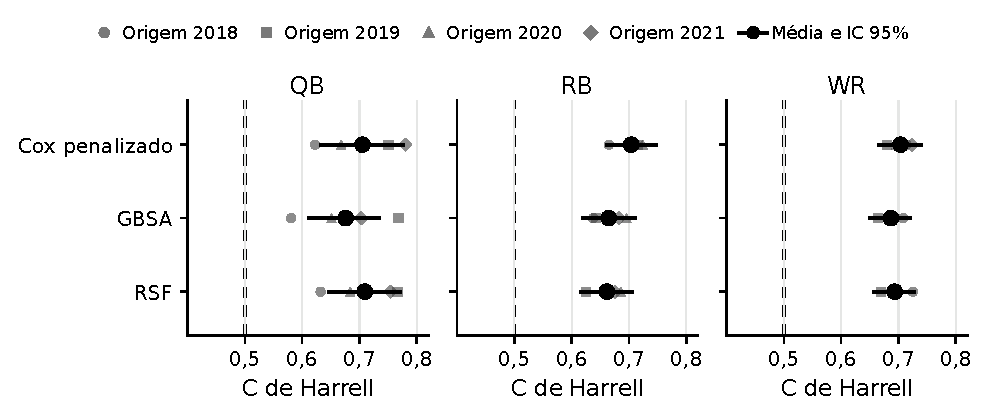
\includegraphics[width=\textwidth,height=0.28\textheight,keepaspectratio]{c_walkforward_folds.pdf}
\caption{C de Harrell por posição e modelo no \textit{walk-forward}. Cada marca colorida é o $C$ de uma origem (2018 a 2021), calculado com todos os pares comparáveis daquela temporada de teste. O ponto preto é a média das quatro origens, e o traço, o IC de 95\% dessa média por \textit{bootstrap} de jogadores ($2\,000$ réplicas): cada réplica sorteia jogadores com reposição e recalcula o $C$ das quatro origens. O intervalo não vem só dos quatro pontos. Tracejado: $C = 0{,}5$, o valor do Kaplan--Meier, que não ordena.}
\label{fig:tgb_wf}
\end{figure}

A figura mostra também que os três modelos ficam próximos, e que só uma vantagem se sustenta. No RB, o Cox fica acima do GBSA e do RSF nas quatro origens, e a diferença para o RSF resiste à correção de Holm nos contrastes pareados ($p$ ajustado de $0{,}016$; Tabela~\ref{tab:tgb_delta}). No QB, RSF e Cox empatam, e só o GBSA fica para trás. No WR, nenhum modelo se separa dos demais. Dentro de cada posição, a diferença de $C$ entre os modelos não passa de $0{,}05$: a forma do modelo pesa menos que a informação do retrato.

Essa informação vai além do tempo de carreira. Um Cox só com a experiência tem $C$ médio entre $0{,}563$ e $0{,}620$, e as demais covariáveis do retrato somam de $0{,}09$ a $0{,}14$ a esse valor. O ganho aparece também na curva prevista, e não só na ordem: o IBS do modelo principal fica de 7\% a 12\% abaixo do Kaplan--Meier nas três posições. E não depende do horizonte desigual das origens: com o desfecho truncado em três anos em todas elas, o $C$ do modelo principal fica entre $0{,}702$ e $0{,}709$.

O modelo usado nas leituras seguintes é o de maior $C$ em cada posição: RSF no QB, Cox no RB e no WR. No RB, a escolha tem apoio do contraste pareado; no QB e no WR, em que os modelos ficam próximos, o maior $C$ decide.

\section{Onde o modelo acerta e onde erra}
\label{sec:acerto_horizonte}

Ordenar bem não garante acertar o prazo. Esta seção mede o erro em anos, verifica em que grupos de risco ele aparece, em que carreiras se concentra e como isso se vê em jogadores concretos.

\subsection{Tamanho do erro e calibração}
\label{sec:calibracao_risco}

A Tabela~\ref{tab:tgb_hit} traz o erro da previsão em anos. Os modelos erram em média cerca de $1{,}3$ ano, pouco menos que o Kaplan--Meier: as covariáveis ajudam mais a ordenar os jogadores do que a acertar o prazo. A média é puxada por uma minoria de erros grandes. A mediana do erro fica abaixo da média em todos os modelos com covariáveis, e cerca de metade das previsões do QB e $40\%$ das do RB e do WR erram por até um ano.

O erro tem direção: os modelos preveem carreira mais longa que a observada, com viés entre $+0{,}28$ e $+0{,}42$ ano nos nove modelos (Tabela~\ref{tab:tgb_hit}). A maior parte desse viés vem da regra de censura, que supõe a saída ao fim da temporada: sem ela, o viés cai para menos de $+0{,}2$ ano (Apêndice~\ref{subsec:apend_censura_pred}). A calibração mostra em que jogadores ele aparece. A Figura~\ref{fig:tgb_calibracao} separa os jogadores em cinco grupos pelo risco que o modelo principal lhes dá, nas origens de 2018 a 2020, e compara a probabilidade prevista de permanecer três anos, $S(3)$, com a observada em cada grupo, estimada por Kaplan--Meier. Na origem de 2021, o acompanhamento termina em três anos, e $S(3)$ não é calculada.

Nela, previsão e observação caem juntas do grupo de menor para o de maior risco, o que confirma a ordenação. A linha, porém, tende a ficar acima das marcas. No RB e no WR, o grupo de menor risco é bem calibrado, e nos demais a permanência prevista supera a observada, em até $0{,}23$. No QB, a diferença chega a $0{,}17$. No RB e no WR, parte dessa distância vem da penalização do Cox, que encolhe os coeficientes e aproxima as previsões da média, efeito que a Seção~\ref{sec:landmark_leitura} mede. Na prática, a ordem entre os grupos é confiável, e a probabilidade é otimista: os grupos de maior risco parecem mais estáveis do que são.

\begin{table}[H]
\centering
\caption{Erro do tempo previsto em anos no \textit{walk-forward}, origens 2018 a 2021: erro absoluto médio (MAE), viés (média de previsto menos observado; positivo indica carreira prevista mais longa que a observada), mediana do erro absoluto e percentual de erro até 1 e 3 anos.}
\label{tab:tgb_hit}
\thesistablesetup\footnotesize
\begin{tabular*}{\textwidth}{@{\extracolsep{\fill}}llccccc@{}}
\toprule
\textbf{Pos.} & \textbf{Modelo} & \textbf{MAE} & \textbf{Viés} & \textbf{Mediana do erro} & \textbf{Erro até 1 ano} & \textbf{Erro até 3 anos} \\
\midrule
QB & Kaplan--Meier & 1{,}48 & $+0{,}18$ & 1{,}26 & 34{,}7\% & 91{,}1\% \\
QB & Cox           & 1{,}30 & $+0{,}30$ & 0{,}94 & 52{,}8\% & 90{,}0\% \\
QB & GBSA          & 1{,}37 & $+0{,}42$ & 1{,}02 & 49{,}4\% & 90{,}4\% \\
QB & RSF           & 1{,}27 & $+0{,}28$ & 0{,}94 & 52{,}0\% & 91{,}1\% \\
\midrule
RB & Kaplan--Meier & 1{,}41 & $+0{,}23$ & 1{,}47 & 38{,}9\% & 95{,}1\% \\
RB & Cox           & 1{,}32 & $+0{,}40$ & 1{,}25 & 40{,}5\% & 97{,}1\% \\
RB & GBSA          & 1{,}38 & $+0{,}39$ & 1{,}24 & 37{,}0\% & 97{,}1\% \\
RB & RSF           & 1{,}29 & $+0{,}33$ & 1{,}18 & 40{,}9\% & 96{,}3\% \\
\midrule
WR & Kaplan--Meier & 1{,}52 & $+0{,}24$ & 1{,}46 & 35{,}9\% & 95{,}1\% \\
WR & Cox           & 1{,}38 & $+0{,}41$ & 1{,}24 & 40{,}3\% & 93{,}7\% \\
WR & GBSA          & 1{,}40 & $+0{,}41$ & 1{,}24 & 39{,}6\% & 93{,}9\% \\
WR & RSF           & 1{,}31 & $+0{,}37$ & 1{,}15 & 44{,}8\% & 95{,}1\% \\
\bottomrule
\end{tabular*}
\end{table}

\begin{figure}[H]
\centering
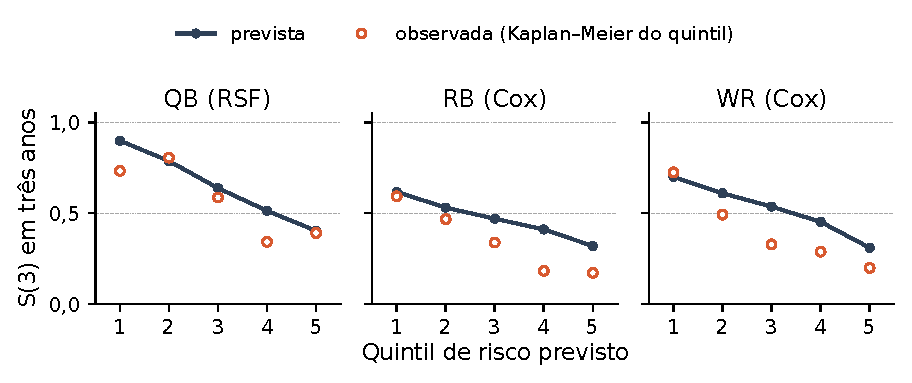
\includegraphics[width=\textwidth]{tgb_calibracao_quintil.pdf}
\caption{Calibração do modelo principal de cada posição no \textit{walk-forward}, origens 2018 a 2020. Os jogadores são divididos em cinco grupos (quintis) pelo risco previsto, do menor (1) ao maior (5). Linha: probabilidade prevista de seguir na liga por mais três anos, $S(3)$, no grupo. Marcas vazadas: a mesma probabilidade observada no grupo, por Kaplan--Meier. Linha acima das marcas indica previsão otimista naquele grupo.}
\label{fig:tgb_calibracao}
\end{figure}

\subsection{Em que carreiras o erro se concentra}
\label{sec:onde_como}

Para ver quem está por trás desse viés, cada par jogador-origem recebe um tipo de trajetória, por regras fixas aplicadas nesta ordem: o par fica com o primeiro tipo cuja regra ele cumpre. \textbf{Além do horizonte}: seguiu na liga até $\tau$, e por isso o erro é negativo por construção, já que a média não passa de $\tau$. \textbf{Hiato}: teve ao menos uma temporada sem jogar entre a primeira e a última da carreira. \textbf{Saída após queda}: a participação ofensiva caiu em duas temporadas seguidas, até a última. \textbf{Saída abrupta}: na última temporada, a participação ofensiva ou a produção da posição estava acima da mediana da posição naquele ano. \textbf{Outras saídas}: as demais. As regras usam o desfecho e a carreira inteira, inclusive os anos posteriores à origem, e servem para mostrar onde o erro cai (Tabela~\ref{tab:tgb_tip}).

\begin{table}[H]
\centering
\caption{Viés médio do modelo principal de cada posição (RSF no QB, Cox no RB e no WR) por tipo de trajetória no \textit{walk-forward}, em anos (previsto menos observado); entre parênteses, o número de pares.}
\label{tab:tgb_tip}
\thesistablesetup
\begin{tabular*}{\textwidth}{@{\extracolsep{\fill}}lccc@{}}
\toprule
\textbf{Tipo} & \textbf{QB} & \textbf{RB} & \textbf{WR} \\
\midrule
Além do horizonte  & $-0{,}84$ (140) & $-1{,}32$ (134) & $-1{,}21$ (266) \\
Hiato              & $+0{,}74$ (62)  & $+0{,}85$ (62)  & $+0{,}68$ (106) \\
Saída após queda   & $+2{,}43$ (14)  & $+0{,}93$ (101) & $+1{,}21$ (127) \\
Saída abrupta      & $+2{,}23$ (27)  & $+1{,}07$ (82)  & $+1{,}58$ (95)  \\
Outras saídas      & $+1{,}85$ (28)  & $+1{,}12$ (132) & $+1{,}43$ (187) \\
\midrule
Todos os pares     & $+0{,}28$ (271) & $+0{,}40$ (511) & $+0{,}41$ (781) \\
\bottomrule
\end{tabular*}
\end{table}

O viés é negativo em quem seguiu além do horizonte e positivo em todos os tipos de saída: quando o jogador sai, o modelo previa mais carreira do que a observada. O erro é maior no QB, perto de dois anos ou mais nos três tipos de saída, e fica perto de um ano no RB e de um ano e meio no WR. O viés não se concentra em um tipo de saída: aparece tanto em quem saiu depois de perder espaço quanto em quem saiu produzindo.

\subsection{Casos no auge}
\label{sec:casos_reais}

A Figura~\ref{fig:tgb_casos} mostra o erro em carreiras concretas do \textit{walk-forward}. São quatro jogadores por posição, todos titulares e entre os dez melhores da posição em jardas na temporada de origem. Em cada linha, as marcas coloridas são os anos previstos pelos três modelos, e o ponto preto, os anos até a saída observada. Os casos foram escolhidos pelo desfecho: ilustram o erro, e não o medem.

A previsão acerta quando o retrato da origem se mantém, e as marcas ficam junto do ponto preto. Kirk Cousins, em 2020, era um titular de 32 anos que quase não perdia jogos: o RSF previu $3{,}9$ anos, e ele seguiu ativo até o fim do horizonte, de quatro anos. Para David Johnson, em 2018, o Cox previu $4{,}1$ anos, e ele saiu após quatro.

O erro típico é a saída que o retrato não anuncia, com as marcas à direita do ponto preto. Philip Rivers, em 2019, tinha 37 anos, 4.615 jardas e nenhum jogo perdido desde 2012: o RSF previu $4{,}4$ anos, e ele jogou só mais uma temporada. Para Leonard Fournette, em 2021, o Cox previu $2{,}4$ anos, e ele saiu após um. São jogadores com produção de quem continua, e é desse tipo de carreira que vem o viés positivo da Tabela~\ref{tab:tgb_tip}. O erro oposto também ocorre: para Mike Evans, em 2018, o Cox previu $4{,}2$ anos, e ele seguia ativo em 2024, além do horizonte de seis anos.

\begin{figure}[H]
\centering
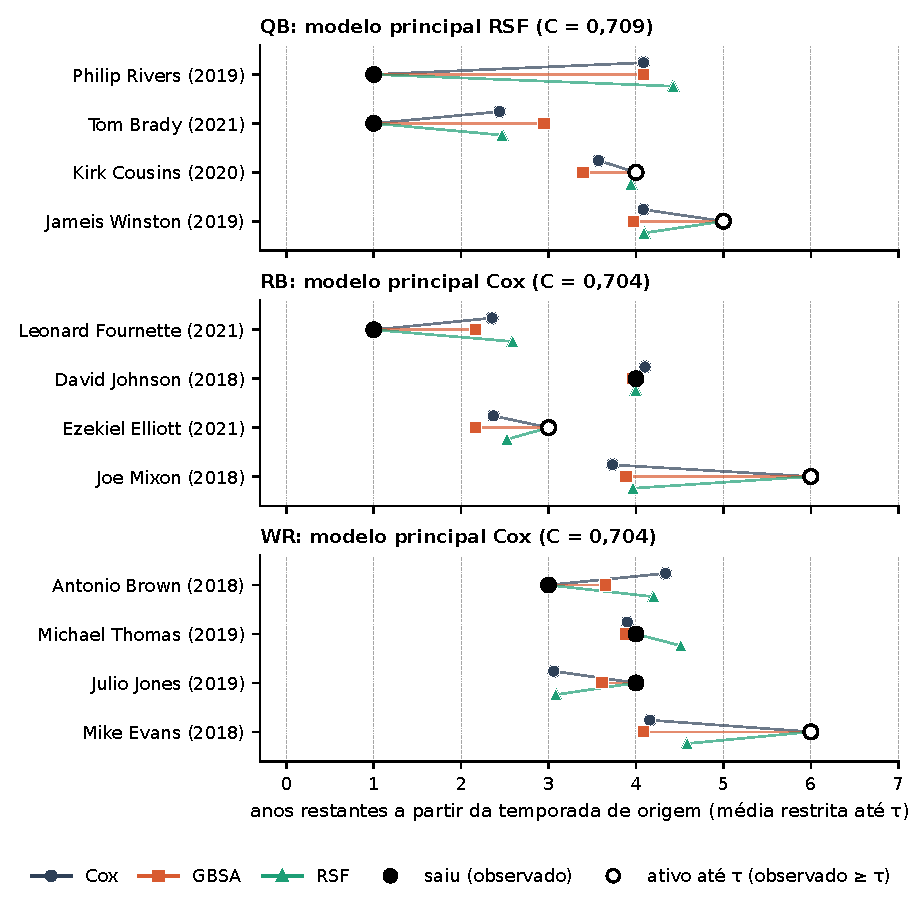
\includegraphics[width=\textwidth,height=0.6\textheight,keepaspectratio]{tgb_casos_leitura.pdf}
\caption{Casos no auge no \textit{walk-forward}, um painel por posição; cada linha é um jogador, com a temporada de origem entre parênteses. Marcas coloridas: anos restantes previstos por Cox (círculo), GBSA (quadrado) e RSF (triângulo). Ponto preto: anos até a saída observada. Círculo vazado: o jogador seguiu ativo até o horizonte $\tau$, então a carreira restante é pelo menos esse valor. O $C$ no título de cada painel é a média do modelo principal no \textit{walk-forward} de 2018 a 2021.}
\label{fig:tgb_casos}
\end{figure}

\section{Quem sai nos próximos anos}
\label{sec:landmark_leitura}

O \textit{walk-forward} responde quanto tempo resta. Para quem decide renovar um contrato por um ou dois anos, a pergunta é outra: entre os jogadores ativos na temporada $s_L$, quem sai da liga nos próximos $w$ anos. É o que o \textit{landmarking} \citep{van_houwelingen2007} mede. Só entram as origens em que a saída em $w$ anos pode ser confirmada, isto é, em que a base cobre a temporada $s_L + w + 1$ (Seção~\ref{subsec:landmarking}): de 2020 a 2022 com $w=1$, 2020 e 2021 com $w=2$ e 2020 com $w=3$. Nessas origens, o $C$ fica entre $0{,}66$ e $0{,}78$ (Apêndice~\ref{sec:ap_landmark}). O desfecho é cortado em $w$, e por isso esse $C$ não se compara ao do \textit{walk-forward}: parte da alta vem do próprio desfecho, mais curto, e parte, do modelo reajustado para o horizonte.

A Figura~\ref{fig:tgb_landmark_quintis} mostra a leitura prática. Dentro de cada origem, os jogadores são repartidos em cinco grupos pelo risco previsto pelo modelo principal, e comparamos, grupo a grupo, a saída prevista e a observada em $w$ anos.

\begin{figure}[H]
\centering
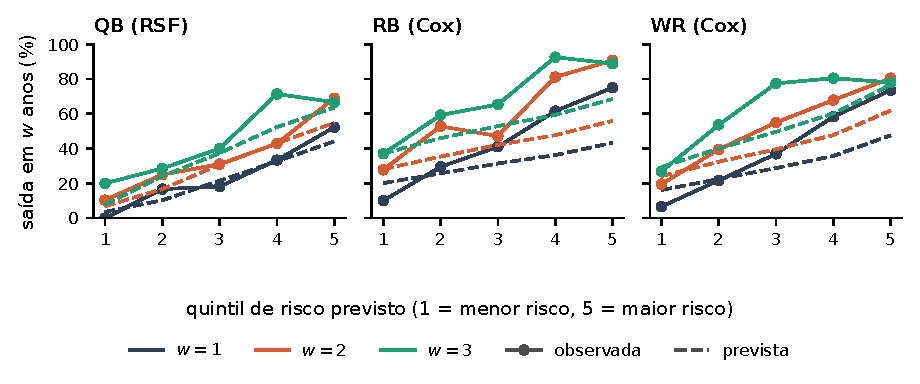
\includegraphics[width=\textwidth,height=0.3\textheight,keepaspectratio]{tgb_landmark_quintis.pdf}
\caption{\textit{Landmarking} com o modelo principal: percentual de saída em $w$ anos por quintil de risco previsto, formado dentro de cada origem (1 = menor risco, 5 = maior). Linha cheia com marcas: saída observada. Linha tracejada: probabilidade média de saída prevista pelo modelo. Cores: horizonte $w$ de 1, 2 e 3 anos.}
\label{fig:tgb_landmark_quintis}
\end{figure}

A saída observada cresce do grupo de menor para o de maior risco, nos três horizontes. Com $w=1$, em que o $C$ é o mais alto (Tabela~\ref{tab:tgb_lm}), saem 52\% dos QBs, 75\% dos RBs e 74\% dos WRs do grupo de maior risco, contra no máximo 10\% no grupo de menor risco. Essa saída soma duas decisões de elenco: não voltar na temporada seguinte, ou jogá-la e não voltar depois. Só a primeira já atinge cerca de metade do grupo de maior risco (45\%, 52\% e 50\%) e quase ninguém no de menor risco. A ordem dada pelo modelo serve, portanto, para separar quem está perto da saída.

A probabilidade prevista é mais tímida que a ordem. No RB e no WR, o Cox comprime os extremos: prevê menos de 50\% de saída no grupo em que cerca de 75\% saem, e prevê mais saída do que ocorre no grupo de menor risco. No QB, o RSF fica mais perto do observado, com 44\% previstos contra 52\%. É o padrão já visto na calibração do \textit{walk-forward} (Seção~\ref{sec:calibracao_risco}), em que o grupo de maior risco parece mais estável do que é, e a penalização $L_2$, que encolhe os coeficientes, explica parte dele no Cox: sem ela, o Cox prevê 55\% e 59\% de saída no grupo de maior risco, sem ganho de $C$. O que se lê com segurança é a posição do jogador entre os grupos, e não a probabilidade.

A origem de 2023 fica fora das médias, porque a saída ao fim de 2024 não pode ser confirmada, mas nela já se sabe quem não voltou em 2024, e os casos repetem o padrão da Seção~\ref{sec:casos_reais}. Os maiores riscos de RB e WR, Brandon Bolden (58\%) e Keith Kirkwood (66\%), vinham de temporadas com dez ou mais jogos perdidos e não jogaram em 2024. Aaron Rodgers, que perdeu 16 jogos em 2023, teve o segundo maior risco entre os QBs (55\%) e voltou. No sentido oposto, Zach Wilson (6\%) era titular e não jogou em 2024, sem que o retrato indicasse isso.

\section{O que sustenta as previsões}
\label{sec:concordancia}

Os três modelos têm formas muito diferentes. Vale, então, perguntar se ordenam os jogadores do mesmo jeito e se usam as mesmas covariáveis para isso.

A Tabela~\ref{tab:tgb_conc} traz a correlação de Spearman entre as previsões de cada par de modelos nas quatro origens do \textit{walk-forward}. Os modelos concordam, e os dois de árvore concordam mais entre si do que com o Cox. Na lista de 2024, em outra população, a correlação fica entre $0{,}88$ e $0{,}98$.

\begin{table}[H]
\centering
\caption{Correlação de Spearman entre as previsões de cada par de modelos no \textit{walk-forward}: média das origens 2018 a 2021.}
\label{tab:tgb_conc}
\thesistablesetup
\begin{tabular*}{\textwidth}{@{\extracolsep{\fill}}lccc@{}}
\toprule
\textbf{Par} & \textbf{QB} & \textbf{RB} & \textbf{WR} \\
\midrule
Cox--GBSA & $0{,}83$ & $0{,}81$ & $0{,}86$ \\
Cox--RSF  & $0{,}88$ & $0{,}86$ & $0{,}89$ \\
GBSA--RSF & $0{,}92$ & $0{,}89$ & $0{,}93$ \\
\bottomrule
\end{tabular*}
\end{table}

A concordância geral esconde desacordos em jogadores específicos. Raheem Mostert, em 2019, é um dos maiores: o GBSA o coloca no percentil 4 do tempo previsto na origem, e o Cox, no percentil 73, mais perto dos cinco anos sem saída que ele teve.

Para ver em que cada modelo se apoia, medimos a queda do $C$ ao permutar cada covariável, que é a medida comparável entre as três famílias. A Tabela~\ref{tab:tgb_imp_inf} traz as covariáveis que ficam entre as cinco primeiras em alguma família, entre as 25 do QB e do WR e as 21 do RB, com a queda no modelo principal.

A ordenação se apoia em poucas covariáveis: no modelo principal, as cinco primeiras respondem por 77\% a 89\% da queda positiva do $C$, e as demais pouco mudam a ordem. O topo tem três temas. O primeiro é o tempo de carreira: a experiência está entre as três mais importantes nas três posições e nos três modelos, como se espera, já que o tempo restante depende do tempo já percorrido.

O segundo tema é o papel na equipe, e o terceiro, a disponibilidade, com peso que muda por posição. No QB, a previsão segue a eficiência e a fatia de passes. No RB, os jogos perdidos ficam em primeiro lugar nos três modelos, seguidos da participação ofensiva. No WR, experiência, jogos perdidos e fatia de alvos se alternam no topo. Os modelos concordam nesse topo e divergem abaixo dele.

\begin{table}[H]
\centering
\caption{Importância por permutação no \textit{walk-forward}: posto em cada modelo (1 = a covariável cuja permutação mais derruba o $C$) e queda do $C$ no modelo principal da posição. Entram as covariáveis que ficam entre as cinco primeiras em algum modelo.}
\label{tab:tgb_imp_inf}
\thesistablesetup
\footnotesize\setlength{\tabcolsep}{3pt}
\begin{tabular*}{\textwidth}{@{\extracolsep{\fill}}llcccc@{}}
\toprule
\textbf{Pos.} & \textbf{Covariável} & \textbf{Cox pen.} & \textbf{GBSA} & \textbf{RSF} & \textbf{Queda do $C$} \\
\midrule
QB & Eficiência de passe (\textit{passer rating}) & 2 & 1 & 1 & $0{,}038$ \\
QB & Fatia de passes da equipe & 3 & 2 & 2 & $0{,}021$ \\
QB & Experiência (anos) & 1 & 3 & 3 & $0{,}015$ \\
QB & Participação ofensiva & 21 & 4 & 4 & $0{,}012$ \\
QB & Profundidade no elenco & 7 & 7 & 5 & $0{,}005$ \\
QB & Hist. defasado jardas por corrida & 5 & 21 & 6 & $0{,}005$ \\
QB & Hiato acumulado na janela & 4 & 6 & 7 & $0{,}004$ \\
QB & Peso & 9 & 5 & 16 & $0{,}000$ \\
\midrule
RB & Jogos perdidos & 1 & 1 & 1 & $0{,}041$ \\
RB & Participação ofensiva & 2 & 2 & 2 & $0{,}026$ \\
RB & Experiência (anos) & 3 & 3 & 3 & $0{,}025$ \\
RB & Fatia de jardas terrestres & 4 & 4 & 4 & $0{,}012$ \\
RB & Hist. defasado YPC & 5 & 6 & 15 & $0{,}010$ \\
RB & Veterano pré-janela & 7 & 5 & 5 & $0{,}006$ \\
\midrule
WR & Experiência (anos) & 1 & 2 & 3 & $0{,}048$ \\
WR & Jogos perdidos & 2 & 3 & 2 & $0{,}045$ \\
WR & Fatia de alvos da equipe & 3 & 1 & 1 & $0{,}021$ \\
WR & Participação ofensiva & 4 & 4 & 4 & $0{,}014$ \\
WR & Veterano pré-janela & 5 & 6 & 5 & $0{,}009$ \\
WR & Hiato acumulado na janela & 6 & 5 & 8 & $0{,}008$ \\
\bottomrule
\end{tabular*}
\end{table}

\section{Aplicação à lista de 2024}
\label{sec:lista_2024}

Com o erro e os sinais conhecidos, a lista de 2024 pode ser lida. Ela reúne os 74 QBs, 107 RBs e 178 WRs ativos naquela temporada e mostra, para cada um, quantos anos de carreira o modelo principal da posição espera: o RSF no QB, e o Cox no RB e no WR, que tiveram o maior $C$ no \textit{walk-forward} de 2018 a 2021. O ajuste segue o mesmo protocolo, com 2024 como origem: o modelo é treinado com as temporadas até 2023 e aplicado ao retrato de 2024. A média é restrita a $\tau = 11$ anos, que é o menor dos maiores seguimentos de treino entre as posições. A base termina em 2024, e a lista não tem desfecho nela: mostra o que o modelo espera de quem estava em campo naquele ano. A Figura~\ref{fig:tgb_lista_2024} mostra os seis maiores e os seis menores valores de cada posição, com a mediana da lista marcada.

No topo estão titulares jovens e produtivos. Entre os QBs, Lamar Jackson, C.J. Stroud e Jalen Hurts estão entre os seis primeiros, que têm de 22 a 29 anos e recebem do RSF entre $8{,}4$ e $9{,}4$ anos, perto do teto de 11. A ponta não é só de quem é novo: Baker Mayfield, com seis anos de carreira, está no mesmo grupo de Stroud, que tem um, porque o modelo lê a produção junto com o tempo já percorrido. Entre os RBs e os WRs, lideram Devon Achane e Malik Nabers, com cerca de sete anos.

No outro extremo estão reservas quase sem participação em 2024, como Josh Johnson, de 38 anos e 16 de carreira, que teve 17 jardas de passe, e WRs que terminaram a temporada sem jardas de recepção.

\begin{figure}[H]
\centering
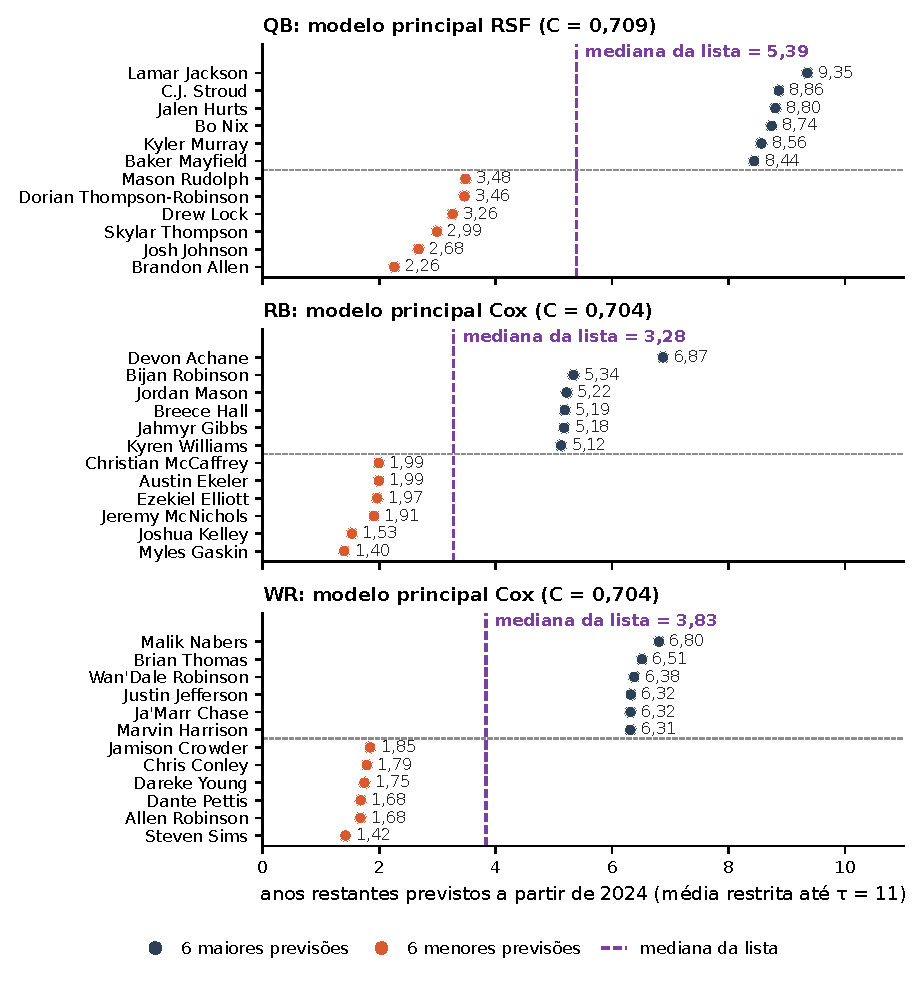
\includegraphics[width=\textwidth,height=0.5\textheight,keepaspectratio]{tgb_lista_2024.pdf}
\caption{Lista de 2024: em cada posição, os seis jogadores com mais anos previstos (azul, acima) e os seis com menos (laranja, abaixo), entre todos os ativos em 2024, pelo modelo principal, treinado com as temporadas até 2023. Previsão: média restrita a 11 anos. Linha tracejada: mediana da lista inteira da posição. O $C$ no título de cada painel é a média do \textit{walk-forward} de 2018 a 2021; a lista não tem desfecho e, por isso, não tem $C$ próprio.}
\label{fig:tgb_lista_2024}
\end{figure}

A Figura~\ref{fig:tgb_lista_quintis} olha a lista inteira, e não só os extremos: os ativos de 2024 são divididos em cinco grupos pelo risco que o modelo principal lhes dá. Do grupo de menor risco para o de maior, a fatia da equipe e a participação ofensiva caem e os jogos perdidos sobem, nas três posições. No QB, por exemplo, a mediana da fatia de passes vai de $0{,}89$ a $0{,}06$. A experiência não segue um padrão único: no RB e no WR, o grupo de maior risco reúne jogadores mais experientes, e no QB a curva oscila. A previsão se apoia, assim, nos mesmos temas da Seção~\ref{sec:concordancia}: o papel na equipe e a disponibilidade.

\begin{figure}[H]
\centering
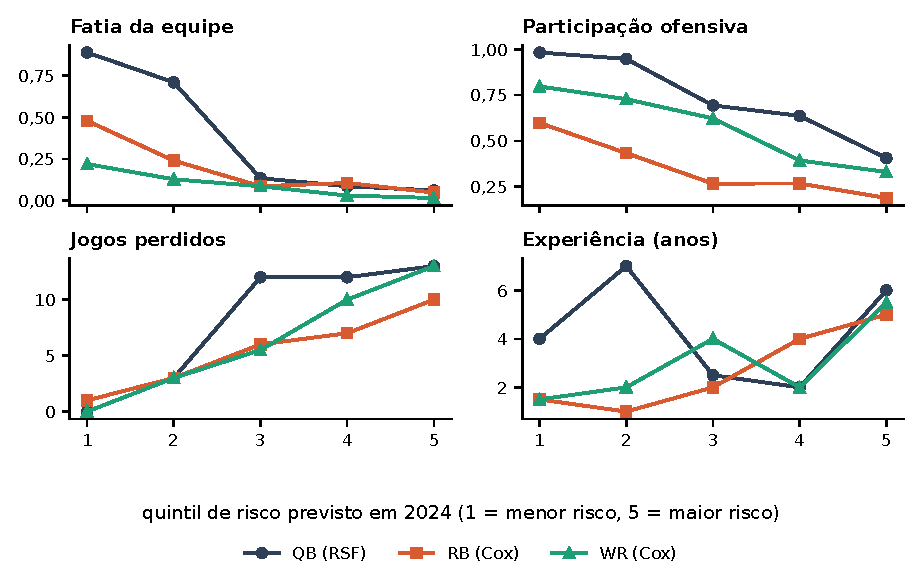
\includegraphics[width=\textwidth,height=0.32\textheight,keepaspectratio]{tgb_lista_quintis.pdf}
\caption{Lista de 2024 por quintil de risco previsto pelo modelo principal (a mesma previsão da Figura~\ref{fig:tgb_lista_2024}): 1 reúne os jogadores com mais anos previstos (menor risco) e 5, os com menos (maior risco). Cada ponto é a mediana do grupo, com todos os ativos de 2024 (cerca de 15 jogadores por grupo no QB, 21 no RB e 36 no WR). Fatia da equipe e participação ofensiva vão de 0 a 1.}
\label{fig:tgb_lista_quintis}
\end{figure}

O erro foi medido com horizontes de 3 a 6 anos, e a lista vai a 11: os anos acima de seis são extrapolação do modelo, e a lista vale pela ordem que dá aos jogadores.

Os modelos nem sempre concordam sobre um jogador: Amon-Ra St. Brown é o 8º WR no Cox e o 20º no GBSA. A lista mede tempo de carreira esperado, não qualidade atual. O que esses sinais significam em risco, e até onde coincidem com a inferência, é o tema do Capítulo~\ref{cap:discussao}.



%%% --- Capítulo 6 --- %%%
% ============================================================
%  Capítulo 6: Discussão
% ============================================================

\chapter{Discussão}
\label{cap:discussao}

Este capítulo interpreta os resultados: o que a inferência sustenta, o que a predição acrescenta, onde as duas se encontram e o que acompanhar em cada posição.

\section{O que a inferência sustenta}
\label{sec:disc_inferencia}

O Cox e o Aalen respondem a perguntas complementares, mesmo com o tempo anual. O Cox dá o efeito de cada covariável em HR, e o Aalen mostra como esse efeito se comporta ao longo da carreira, justamente onde a proporcionalidade não se sustenta. O modelo de tempo discreto, forma exata dos riscos proporcionais para tempo agrupado, concorda com o Cox em sinal e em significância em todos os termos finais (Seção~\ref{sec:res_procedimentos}), de modo que os empates não mudam a leitura.

Nove associações têm $p<0{,}05$ nos três ajustes (Seção~\ref{sec:sintese_inferencial}), e elas mudam de uma posição para outra: não há um perfil único de quem permanece.

No QB, permanece quem produz. A eficiência de passe é o sinal mais firme, com $p<0{,}001$ nos três modelos, e não há evidência contra um HR único. A participação ofensiva se lê junto com a fatia de passes, que está no mesmo modelo.

No RB, pesam a disponibilidade e o lugar no elenco. Nos jogos perdidos, o resultado mais informativo está em como agem: a razão de riscos enfraquece com a carreira, e o risco absoluto é compatível com um acréscimo constante na janela do Aalen. Por isso a leitura útil é esse acréscimo anual, e não o HR único. A posição no \textit{draft} só se separa de zero no Cox. Isso está em linha com \citet{ducking2015}, em que jogos disputados e jogos como titular se associam a carreira mais longa. Sem as covariáveis de uso, o HR da posição no \textit{draft} é bem maior ($1{,}58$; Seção~\ref{subsec:rb}). Isso é compatível com parte da associação passar pelo papel que o jogador recebe, sem separá-la, porque o ajuste não é uma análise de mediação, e contrasta com o efeito persistente que \citet{staw1995} encontraram na NBA.

No WR, o papel de alvo principal é o sinal que mais se repete. A fatia de alvos está associada a menor risco, e a idade e os jogos perdidos, a maior. Como a experiência é o eixo do tempo, a idade indica quem entrou mais velho na liga, e não o envelhecimento.

\section{O que a predição acrescenta}
\label{sec:interpretacao_posicao}

A predição testa se o retrato de uma temporada serve para o futuro, e serve: em toda posição, o modelo ordena os jogadores bem acima do acaso e separa quem está perto da saída. As posições diferem no prazo. O QB tem a carreira restante mais longa. O RB tem a mais curta, e o WR fica entre os dois. O erro em anos não compara posições com segurança, porque depende de $\tau$, da fração além do horizonte e do modelo.

O erro se concentra quando a saída não está no retrato, como em Rivers, que saiu um ano depois de uma temporada de 4.615 jardas, e em Evans, que durou além do previsto. A ordem entre os jogadores é, por isso, a leitura mais firme da previsão, já que o tempo até o evento de cada indivíduo não se prevê bem por si só \citep{graf1999}. No RB e no WR, o Cox também aproxima da média as probabilidades dos extremos, e os grupos de maior risco saem mais do que o previsto.

\section{Onde as duas leituras se encontram}
\label{sec:disc_encontro}

A inferência mede o efeito ajustado numa lista curta, e a permutação mede quanto a ordenação depende da covariável no conjunto completo. Por isso o encontro não se faz com o HR de um modelo: partimos das nove associações da inferência e vemos se elas movem a previsão (Tabela~\ref{tab:leituras_cruzadas}).

As associações da inferência tendem a mover a previsão. Das nove associações, cinco ficam entre as quatro primeiras nas três famílias: a eficiência e a fatia de passes no QB, os jogos perdidos no RB e no WR, e a fatia de alvos no WR. É o núcleo do trabalho: o mesmo sinal acompanha a saída e melhora a ordenação. A idade do WR cai no filtro de colinearidade, e a idade de entrada fica sem representante direto no modelo preditivo. A participação ofensiva do QB oscila do 21º ao 4º lugar, e a profundidade e o YPC do RB ficam no meio da lista. A profundidade, por exemplo, anda junto com a participação ofensiva, que está no topo (Spearman de $-0{,}65$).

\begin{table}[H]
\centering
\caption{Covariáveis do Cox final: sentido do risco, ajustes inferenciais com $p<0{,}05$ (Cox, Aalen, Cox--Aalen) e postos por permutação. Célula vazia: fora do conjunto preditivo.}
\label{tab:leituras_cruzadas}
\thesistablesetup
\footnotesize\setlength{\tabcolsep}{3pt}
\begin{tabular*}{\textwidth}{@{\extracolsep{\fill}}llccccc@{}}
\toprule
\textbf{Pos.} & \textbf{Covariável} & \textbf{Sentido} & \textbf{Ajustes (de 3)} & \textbf{Cox pen.} & \textbf{GBSA} & \textbf{RSF} \\
\midrule
QB & Eficiência de passe & $-$ & 3 & 2 & 1 & 1 \\
QB & Fatia de passes da equipe & $-$ & 3 & 3 & 2 & 2 \\
QB & Participação ofensiva & $+$ & 3 & 21 & 4 & 4 \\
QB & Hist. defasado TD\% & $-$ & 2 & 22 & 24 & 24 \\
QB & Hist. defasado comp\% ausente & $+$ & 2 & 13 & 13 & 17 \\
\midrule
RB & Jogos perdidos & $+$ & 3 & 1 & 1 & 1 \\
RB & Hist. defasado YPC & $-$ & 3 & 5 & 6 & 15 \\
RB & Profundidade no elenco & $+$ & 3 & 6 & 8 & 8 \\
RB & Fatia de jardas terrestres & $-$ & 2 & 4 & 4 & 4 \\
RB & Posição no \textit{draft} & $+$ & 1 & 8 & 7 & 16 \\
\midrule
WR & Fatia de alvos da equipe & $-$ & 3 & 3 & 1 & 1 \\
WR & Jogos perdidos & $+$ & 3 & 2 & 3 & 2 \\
WR & Idade & $+$ & 3 & & & \\
WR & Hist. defasado jardas de corrida & $-$ & 2 & 10 & 22 & 21 \\
WR & Hist. defasado alvos na \textit{red zone} & $-$ & 2 & & & \\
WR & Altura & $+$ & 2 & 19 & 23 & 22 \\
WR & Participação ofensiva & $+$ & 1 & 4 & 4 & 4 \\
\bottomrule
\end{tabular*}
\end{table}

Fora das nove, as leituras se separam nos dois sentidos. O TD\% histórico do QB e a altura e as jardas de corrida do WR quase não movem a ordenação deste conjunto, em que outras covariáveis correlacionadas podem substituí-las. Já a fatia de jardas do RB e a participação ofensiva do WR e do RB ficam no topo das três famílias, com apoio inferencial parcial ou nulo: na predição, elas marcam o papel no elenco.

\section{O que acompanhar em cada posição}
\label{sec:discussao_elenco}

Juntas, as duas leituras dizem o que acompanhar em cada posição e como usar a previsão na avaliação de um elenco.

No QB, o que se acompanha é a produção. A eficiência de passe e a fatia de passes acompanham a saída e movem a previsão, e a eficiência é o sinal mais firme: um QB 21 pontos de \textit{passer rating} acima da média tem cerca de 35\% menos risco. Como a carreira restante é a mais longa, a ordem da lista ajuda a planejar a posição.

No RB, o que se acompanha são a disponibilidade e o lugar no elenco. As ausências se leem como um acréscimo anual de risco, e cada degrau para baixo no \textit{depth chart} está associado a cerca de $23\%$ mais risco, controladas as demais covariáveis, inclusive as ausências. Como a saída é frequente no maior quintil de risco, esse quintil é a leitura mais útil numa decisão de renovação.

No WR, o que se acompanha são o papel de alvo principal e as ausências. As duas covariáveis acompanham a saída nos três ajustes e ficam entre as três primeiras por permutação nas três famílias: cada 5 pontos percentuais a mais de fatia de alvos correspondem a cerca de metade do risco, e cinco jogos perdidos a mais, a cerca de 27\% mais risco. Na lista de 2024, o grupo de maior risco tem participação ofensiva mediana de $0{,}33$, contra $0{,}80$ no de menor risco: é ali que estão os recebedores fora do papel principal.

Nas três posições, esses sinais servem para acompanhar o jogador, e a lista ordena o elenco.

% ============================================================
%  Capítulo 7: Conclusão
% ============================================================

\chapter{Conclusão}
\label{cap:conclusao}

Este trabalho estudou a duração das carreiras de \textit{quarterbacks}, \textit{running backs} e \textit{wide receivers} na NFL entre 2012 e 2024, a partir do retrato anual de cada jogador. A conclusão central é que o retrato de uma temporada acompanha parte da saída e ordena os jogadores bem acima do acaso, com sinais que mudam de uma posição para outra, mas não fixa o prazo de uma carreira.

\section{Respostas aos objetivos}
\label{sec:respostas_objetivos}

\begin{enumerate}
  \item \textbf{Painel de sobrevivência.} Construído no formato \textit{start--stop}, com uma linha por jogador e temporada, covariáveis atualizadas a cada ano e saída definida como a última temporada na liga (Seção~\ref{sec:tratamentos_eda}).
  \item \textbf{Análise descritiva.} A duração mediana é de 7 anos no QB e de 5 no RB e no WR. Nessas duas posições, ela é maior para os selecionados nas primeiras rodadas do \textit{draft}, e, nas três, para quem é titular no primeiro ano observado (Seção~\ref{sec:eda}).
  \item \textbf{Cox por posição.} No QB, a fatia de passes tem o maior efeito em HR, e a eficiência de passe, com HR de $0{,}65$ por desvio-padrão, é o sinal mais estável. No RB e no WR, as ausências se associam a mais risco; no WR, a fatia de alvos se associa a menos, com HR de $0{,}27$ (Seção~\ref{sec:res_posicoes}). O modelo de tempo discreto concorda em sinal e em significância em todos os termos finais (Seção~\ref{sec:res_procedimentos}).
  \item \textbf{Proporcionalidade.} O teste de Schoenfeld rejeita a proporcionalidade global no RB e no WR, por causa das ausências e da fatia da equipe, e não rejeita no QB (Seção~\ref{subsec:schoenfeld}).
  \item \textbf{Aalen.} O efeito acumulado das ausências cresce quase em linha reta no RB e no WR, na janela de cada posição, e o da eficiência do QB desce de forma regular (Seção~\ref{sec:aalen_res}).
  \item \textbf{Leitura conjunta.} Nove associações têm $p<0{,}05$ nos três ajustes: no QB, eficiência de passe, fatia de passes e participação ofensiva; no RB, ausências, profundidade no elenco e eficiência de corrida; no WR, ausências, idade e fatia de alvos. No RB e no WR, o híbrido não rejeita um efeito constante por ano das ausências e da fatia da equipe (Seções~\ref{sec:res_coxaalen} e~\ref{sec:res_lado}).
  \item \textbf{Tempo restante e saída próxima.} O modelo de maior $C$ é o RSF no QB e o Cox penalizado no RB e no WR. O erro absoluto médio fica entre $1{,}27$ e $1{,}40$ ano nos nove modelos, com viés de carreira mais longa que a observada, em grande parte devido à convenção de censura (Apêndice~\ref{subsec:apend_censura_pred}), e o ganho do modelo principal sobre o Kaplan--Meier vai de 6\% a 14\% (Tabela~\ref{tab:tgb_hit}). O \textit{landmarking} separa com clareza quem sai em breve (Seção~\ref{sec:landmark_leitura}). A Tabela~\ref{tab:sintese_preditiva} resume os resultados.
\end{enumerate}

\begin{table}[H]
\centering
\caption{Síntese da predição por posição, com o modelo principal: ordenação, erro, carreira restante esperada em 2024 e quem não volta na temporada seguinte nos quintis extremos de risco.}
\label{tab:sintese_preditiva}
\thesistablesetup
\begin{tabular*}{\textwidth}{@{\extracolsep{\fill}}lccc@{}}
\toprule
 & \textbf{QB (RSF)} & \textbf{RB (Cox)} & \textbf{WR (Cox)} \\
\midrule
$C$ no \textit{walk-forward} & $0{,}709$ & $0{,}704$ & $0{,}704$ \\
Erro absoluto médio (anos) & $1{,}27$ & $1{,}32$ & $1{,}38$ \\
Erro de até um ano & 52,0\% & 40,5\% & 40,3\% \\
Mediana prevista em 2024 (anos) & $5{,}39$ & $3{,}28$ & $3{,}83$ \\
Não volta na temporada seguinte, menor risco & 0\% & 1\% & 2\% \\
Não volta na temporada seguinte, maior risco & 45\% & 52\% & 50\% \\
\bottomrule
\end{tabular*}
\end{table}

\section{Limitações}
\label{sec:limitacoes}

Os resultados se leem dentro do alcance dos dados e dos métodos usados, e os apêndices indicados mostram o efeito de cada escolha.

\begin{itemize}
  \item \textbf{Dados.} São anuais e não registram o motivo da saída, de modo que lesão, contrato e decisão da equipe não se distinguem. A cobertura da base cresce com o tempo: a razão entre jardas recebidas e passadas por equipe tem mediana de 0,84 em 2012 e de cerca de 0,97 desde 2019, e as conclusões valem para esta base (Apêndice~\ref{apx:regras_painel}). Jogos perdidos não distinguem lesão, banco ou corte. A saída é reconhecida pela ausência nas temporadas seguintes, o que torna as saídas de 2023 as de leitura mais delicada. As taxas faltantes seguem uma regra de preenchimento comparada à imputação múltipla (Apêndice~\ref{subsec:imputacao_apend}).
  \item \textbf{Interpretação.} Os resultados são associações, e não efeitos causais. As covariáveis de temporada descrevem o último ano antes da saída e podem refleti-la. Com a temporada anterior no lugar da corrente, a eficiência do QB e os jogos perdidos do RB se mantêm, e a fatia e a participação do QB e os jogos perdidos do WR deixam de ser significativos (Apêndice~\ref{subsec:apend_temp_ant}). O \textit{draft} e o lugar no elenco refletem também a avaliação dos times.
  \item \textbf{Seleção.} As listas finais vêm dos mesmos dados da estimação, o que pede leitura cuidadosa dos valores-$p$ e dos HR \citep{harrell2001}, e os três modelos inferenciais usam os mesmos dados, de modo que a concordância entre eles não é replicação. A triagem do Aalen refeita com as linhas ordenadas está no Apêndice~\ref{subsec:apend_janela}. A frequência de cada covariável em reamostras está no Apêndice~\ref{subsec:apend_frequencia}.
  \item \textbf{Aalen.} É estimado na faixa de anos com posto completo e descreve a parte intermediária da carreira (Apêndice~\ref{subsec:apend_janela}).
  \item \textbf{Predição.} O $C$ mede ordenação, e por isso o acompanhamos com o IBS e o erro em anos. Os intervalos dos contrastes reamostram jogadores com as predições fixas. No QB, de menor amostra, a ordem entre os modelos muda de uma origem para outra. A base termina em 2024, e a lista não tem desfecho nela.
\end{itemize}

\section{Trabalhos futuros}
\label{sec:futuros}

Três direções se destacam. A primeira é incorporar dados de lesão e de contrato, para separar o motivo da saída e tratar cada motivo como um risco próprio. A segunda é acompanhar a lista de 2024 nas próximas temporadas, o que dará desfecho a essas previsões. A terceira é estender o estudo a outras posições, como linha ofensiva, \textit{tight ends} e defesa, para ver se o padrão de ausências e de papel na equipe se repete.

\section{Código e reprodutibilidade}
\label{sec:codigo}

Todo o código deste trabalho está em repositório público \citep{gon2026codigo}: a construção do painel, a análise exploratória, os modelos inferenciais e preditivos, as sensibilidades dos apêndices e a geração das tabelas e das figuras. O repositório traz também os resultados que sustentam cada número do texto, e uma rotina única refaz toda a análise a partir da base de dados.


%%% --- Apêndices --- %%%
\appendix
\chapter{Detalhes dos dados}\label{apx:cap_dados}
% ============================================================
%  Apêndice A: dados, painel e tratamento de ausências (para \input)
% ============================================================

\section{Dados, painel e tratamento de dados faltantes}
\label{apx:dados}

\subsection{Glossário das variáveis}
\label{apx:glossario}

A Tabela~\ref{tab:variaveis} traz o nome de cada variável no texto, o nome no banco e a definição usada. As defasagens acumulam até a temporada $t-1$.

\begingroup
\thesistablesetup
\setlength{\tabcolsep}{4pt}
\renewcommand{\arraystretch}{1.05}
\begin{longtable}{@{}>{\raggedright\arraybackslash}p{4.3cm}>{\raggedright\arraybackslash}p{5.6cm}>{\raggedright\arraybackslash}p{4.9cm}@{}}
\caption{Glossário: nome no texto, nome no banco e definição de cada variável usada na modelagem e nas figuras.}
\label{tab:variaveis}\\
\toprule
\textbf{Nome no trabalho} & \textbf{Nome no banco} & \textbf{Descrição} \\
\midrule
\endfirsthead
\multicolumn{3}{@{}l}{\small\textit{Tabela~\ref{tab:variaveis}, continuação.}}\\
\toprule
\textbf{Nome no trabalho} & \textbf{Nome no banco} & \textbf{Descrição} \\
\midrule
\endhead
\bottomrule
\endfoot
Jogos perdidos & \textit{games\_missed} & 16 ou 17 menos os jogos disputados na temporada, com mínimo zero; inclui lesão, banco e jogos depois de um corte. \\
Profundidade no elenco & \textit{depth\_team} & Posição na hierarquia do time (1 = titular). \\
Participação ofensiva & \textit{offense\_pct} & Fração dos \textit{snaps} ofensivos do time em que o jogador esteve. \\
Eficiência de passe & \textit{passer\_rating} & Índice composto de eficiência do passe (QB). \\
Fatia de passes & \textit{team\_pass\_\newline attempts\_share} & Fração das tentativas da equipe atribuídas ao QB. \\
Fatia de alvos & \textit{team\_targets\_share} & Fração dos alvos da equipe recebidos pelo WR. \\
Fatia de jardas terrestres & \textit{team\_rushing\_\newline yards\_share} & Fração das jardas terrestres da equipe obtidas pelo RB. \\
Posição no \textit{draft} & \textit{draft\_ovr} & \textit{Pick} geral no \textit{draft}; 0 para não draftado. \\
Não draftado & \textit{undrafted\_flag} & Indicador de não ter sido selecionado no \textit{draft}. \\
Anos de experiência & \textit{years\_exp} & Tempo do modelo de Cox (anos desde o início da carreira). \\
Veterano pré-janela & \textit{pre\_window\_veteran} & Carreira iniciada antes de 2012. \\
Histórico defasado & \textit{observed\_career\_lag\_*} & Acumulado de carreira até $t-1$ (TD\%, comp\%, YPC, jardas e outros). \\
Idade & \textit{age} & Idade do jogador na temporada. \\
Altura & \textit{height} & Altura do jogador. \\
Peso & \textit{weight} & Peso do jogador. \\
Anos sem estatísticas antes da 1ª linha & \textit{unobs\_career\_years} & Anos de carreira (\textit{years\_exp}) que antecedem a primeira linha observada e não têm linha no painel. \\
Primeira linha com anos sem estatísticas & \textit{unobserved\_history\_flag} & Primeira linha observada de jogador com anos sem estatísticas antes dela. \\
Hiato acumulado na janela & \textit{within\_window\_gap\_\newline years\_before\_t} & Temporadas de ausência acumuladas dentro da janela até $t$. \\
Alvos na \textit{red zone} & \textit{targets\_redzone} & Alvos a menos de 20 jardas da linha de gol; histórico defasado. \\
Hiato anterior & \textit{had\_prior\_gap\_flag} & Já teve temporada sem jogar antes de $t$. \\
Indicador de dado faltante & \textit{observed\_career\_lag\_*\_missing} & Taxa de carreira não calculada até $t-1$. \\
Primeira temporada observada & \textit{first\_observed\_season} & Indicador da primeira temporada do jogador no painel (ramo preditivo). \\
\end{longtable}
\endgroup

\subsection{Regras do painel e saídas de 2023}
\label{apx:regras_painel}

Trocar jogos perdidos pela fração da temporada, por causa do calendário de 17 jogos desde 2021, não muda nenhum HR em mais de $0{,}01$ nem o lado de 5\%. Três jogadores têm apenas temporada de \textit{playoffs} no último ano (Steven Jackson, Marshawn Lynch e Andy Isabella), e a saída deles é marcada na última temporada regular. São 3 de 790 saídas.

\paragraph{Cobertura da base.}
A razão entre as jardas recebidas e as passadas por equipe, na própria base, tem mediana de $0{,}84$ em 2012, $0{,}92$ em 2016 e cerca de $0{,}97$ desde 2019. A falha também atinge equipes e jogadores isolados: no Saints de 2017, a razão é de $0{,}64$. Como a saída é reconhecida pela falta de temporadas, a menor cobertura inicial pode gerar falsas saídas e hiatos e alterar as fatias da equipe. Com o Cox final ajustado só a partir de 2018, nenhum HR muda de sinal; entre as nove associações, a profundidade do RB e os jogos perdidos do WR deixam de ser significativos a 5\% ($p=0{,}093$ e $0{,}267$), com menos saídas.

\paragraph{Saídas de 2023.}\label{subsec:apend_2023}
Censurar as saídas de 2023, que não têm temporada seguinte para checar o retorno, é a alternativa testada. O número de saídas cai de $107$ para $94$ no QB, de $289$ para $253$ no RB e de $394$ para $343$ no WR. O QB mantém as conclusões, o RB perde profundidade e \textit{draft}, e o WR perde participação ofensiva; das nove associações, só a profundidade do RB deixa de ser significativa a 5\% no Cox. O HR da fatia de alvos do WR vai de $0{,}27$ para $0{,}34$. Censurar também as de 2022 dá o mesmo resultado entre as nove, e nenhum HR muda de sinal. Na métrica $C$ de Harrell, a mudança é de no máximo $0{,}008$, no Cox do WR, e o modelo de maior $C$ continua o mesmo.

\paragraph{Censura no início do intervalo.}\label{subsec:apend_censura_inicio}
Quem é censurado jogou até o tempo $t$, sem que se saiba se saiu depois dele, e o painel o mantém em risco em $t$, como em \citet{ducking2015}. \citet{prentice1978} censuram no início do intervalo. Retirando a última linha de cada censurado (75 no QB, 108 no RB e 179 no WR), nenhum HR muda de sinal, e dois termos deixam de ser significativos a 5\%: o indicador de comp\% ausente do QB ($p$ de $0{,}036$ para $0{,}106$) e a \textit{red zone} do WR ($p$ de $0{,}007$ para $0{,}116$). Refeita a seleção, a lista do RB não muda, a do QB perde esse indicador (Jaccard de $0{,}80$; o índice é a razão entre os termos em comum e o total), e a do WR perde a \textit{red zone} e a participação ofensiva e ganha a posição no \textit{draft} (Jaccard de $0{,}63$). A mediana do Kaplan--Meier passa de 5 para 4 anos no RB e no WR, e fica em 7 no QB.

\subsection{Jogadores com mais de um time na temporada}
\label{apx:multitime}

Há $104$ pares jogador-temporada com mais de um time nas posições do painel: $8$ no QB, $45$ no RB e $51$ no WR, de $1\%$ a $3\%$ de cada posição. Cada par entra como uma linha. As colunas de temporada e de carreira recebem o máximo entre as passagens, porque cada passagem já traz o total da temporada, e somar dobraria esses valores. Posição e taxas vêm da passagem com mais \textit{snaps}. Na base completa, há $119$ pares de temporada regular, e em todos os totais coincidem entre os times, de modo que o máximo só evita a duplicação.

\subsection{Imputação e dados faltantes}
\label{subsec:imputacao_apend}

A regra de preenchimento está na Seção~\ref{subsec:imputacao}. No QB final, fica o indicador da taxa de passes completos. Como preencher com a média geral e o método do indicador podem enviesar as estimativas em estudos não randomizados \citep{donders2006,groenwold2012}, a regra é comparada a seguir com outras escolhas.

\paragraph{Limiar das taxas.}\label{subsec:apend_limiar}
As taxas só são calculadas quando o denominador passa de $50$ oportunidades. Refizemos o painel e a seleção em cada limiar de $25$ a $100$, em passos de $5$. A seleção é a mesma de $50$ no QB de $25$ a $90$, no RB de $25$ a $60$ e no WR de $40$ a $100$. O índice de Jaccard compara a lista de cada variação ($X$) e a principal ($Y$): $J = |X\cap Y|/|X\cup Y|$, em que $J=1$ significa listas iguais. Fora dessas faixas, mudam uma ou duas covariáveis (Jaccard de $0{,}60$ a $0{,}88$).

\paragraph{Eficiência sem tentativa.}
Em $26$ linhas do QB ($3\%$) não houve tentativa, e a eficiência não existe. A mediana global, adotada, foi comparada a zero e à exclusão das linhas. A exclusão tira $26$ linhas e $7$ saídas. O HR da eficiência é $0{,}65$, $0{,}63$ e $0{,}60$, nessa ordem, com $p < 10^{-5}$ nos três casos.

\paragraph{Imputação múltipla com o desfecho.}
Geramos $m = 10$ cópias do conjunto de ajuste, com imputação iterativa e amostragem posterior das ausências das covariáveis finais (TD\% defasado e eficiência do QB; YPC defasado do RB). Seguindo \citet{white2009}, o modelo de imputação inclui o desfecho: o indicador de saída do intervalo e o risco acumulado de Nelson--Aalen, que não entram no Cox. Os coeficientes são combinados pelas regras de Rubin \citep{rubin1987}: a média das $m$ estimativas e a variância total $T = \bar{U} + (1 + 1/m)B$, em que $\bar{U}$ é a variância média dentro das cópias e $B$ a variância entre elas. Com a versão múltipla, nenhuma conclusão muda no QB nem no RB, e o erro-padrão cresce no máximo $6{,}6\%$. No WR, nenhuma covariável final tem ausência. Frente ao ajuste único sem o indicador de ausência, o maior deslocamento do HR é de $6\%$, na fatia de passes do QB. Frente ao ajuste principal, o HR do TD\% defasado sobe $11\%$. Esse aumento vem da retirada do indicador de ausência, e não da imputação: o ajuste único sem o indicador já dá $0{,}70$.

\subsection{Não draftados}
\label{apx:undrafted}

Testamos quatro codificações para não draftados: a usada no ajuste (A); \textit{pick} sem zerar, preenchido pela mediana (B); código $9$ no lugar do código $8$ da rodada (C); e só o indicador, sem \textit{pick} nem rodada (D). A seleção do QB não muda em nenhuma. No RB, B acrescenta o indicador de veterano pré-janela, e D troca o \textit{pick} por esse indicador (Jaccard de $0{,}83$ e $0{,}67$). No WR, B acrescenta esse indicador e retira o acúmulo de alvos na \textit{red zone} (Jaccard de $0{,}75$). A codificação C não altera nenhuma seleção. Mantemos A, que não trata o não draftado como escolha de rodada média. Sem o indicador no modelo, como no Cox do RB, o HR não se lê por \textit{pick}.


\chapter{Detalhes da inferência}\label{apx:cap_inferencia}
% ============================================================
%  Apêndice B: escolhas da parte inferencial (para \input após o Capítulo 4)
%  Referência de entrada: sec:apend_inferencia
% ============================================================

\section{Escolhas da inferência}
\label{sec:apend_inferencia}

\subsection{Experiência como tempo e Cox sem penalização}
\label{subsec:apend_years_exp}

No Cox, o tempo é a própria experiência, por isso \texttt{years\_exp} não entra como covariável. Em cada tempo de saída, todas as linhas em risco têm o mesmo valor. No QB, no tempo $11$, há $34$ linhas em risco, todas com experiência $10$, e $7$ saídas. Uma coluna constante no conjunto de risco não contribui para a verossimilhança parcial e deixa a matriz singular. Esse efeito já está na linha de base, que o Cox estima tempo a tempo.

O modelo final não usa penalização. Com penalização $L_2$, o coeficiente de \texttt{years\_exp} vai a zero para qualquer $\lambda > 0$, sem mudar os demais. Mas, no \texttt{lifelines} \citep{lifelines}, a penalização é multiplicada pelo número de linhas e encolhe os demais coeficientes. Como sensibilidade, com $\lambda = 0{,}1$ o HR da fatia de passes do QB vai de $0{,}29$ para $0{,}75$, e a seleção do QB cai para Jaccard de $0{,}5$. Com $\lambda = 0{,}1$, a seleção também muda no RB (Jaccard de $0{,}67$, com a participação ofensiva no lugar do \textit{draft}) e no WR (Jaccard de $0{,}75$, com a profundidade no lugar da idade). Com $\lambda = 0{,}01$, só a seleção do WR muda, com uma covariável a menos (Jaccard de $0{,}86$). A estimativa sem penalização coincide com a de uma implementação independente, com diferença máxima de $3\cdot10^{-10}$.

\subsection{Empates e tempo discreto}
\label{subsec:apend_empates}

Como o tempo é anual, $97\%$ das saídas do QB, $99{,}7\%$ do RB e $99{,}5\%$ do WR empatam com outra saída, caso em que \citet{grambsch1994} advertem para viés nas estimativas de $\beta(t)$ a partir dos resíduos, e por isso só a direção é usada.

No tratamento de Breslow \citep{breslow1974}, a verossimilhança parcial é
\begin{equation}
    L_{\mathrm{B}}(\boldsymbol{\beta})
    = \prod_{k=1}^{D}
      \frac{\exp\!\left(\boldsymbol{\beta}^{\top}\mathbf{S}_k\right)}
           {\left[\sum_{j \in \mathcal{R}(t_{(k)})} \exp\!\left(\boldsymbol{\beta}^{\top}\mathbf{X}_j\right)\right]^{d_k}},
    \label{eq:pl_breslow}
\end{equation}
em que cada saída empatada é comparada com o conjunto de risco inteiro, e o viés cresce quanto mais grosso é o agrupamento do tempo \citep{prentice1978}. O de Efron \eqref{eq:pl_efron} desconta do conjunto de risco uma fração dos que saem no mesmo tempo, e é um pouco mais preciso \citep{efron1977}, diferença que importa com muitos empates, como aqui. O ajuste principal usa Efron.

Com Breslow, os coeficientes encolhem de $4\%$ a $29\%$, e seis termos deixam de ter $p < 0{,}05$; com Efron, eles tinham $p$ entre $0{,}013$ e $0{,}039$. O sinal de todos os efeitos se mantém. Para decidir entre as duas aproximações, a referência é o modelo exato de tempo discreto, descrito a seguir.

O estimador de Aalen \eqref{eq:aalen_est} regride, em cada tempo de saída, os indicadores sobre as covariáveis do conjunto de risco. Ordenar artificialmente as saídas de um mesmo ano as empurraria para o ano seguinte, e tiraria do conjunto de risco quem terminou a temporada sem sair. Por isso as saídas de cada ano são tratadas em bloco, contra o elenco daquele ano. No RB, há $34$ saídas no tempo $4$ contra $182$ linhas em risco. Em bloco, cada incremento é a regressão linear do indicador de saída naquele ano (diferença menor que $10^{-13}$), de modo que o Aalen já é um modelo discreto aditivo. Um modelo de probabilidade linear agregado, com efeito fixo por ano e erro por jogador, concorda com ele a 5\% em 29 das 32 covariáveis.

\paragraph{Tempo discreto.}\label{subsec:apend_discreto}
Para tempo agrupado, o modelo de riscos proporcionais equivale a um modelo binomial com ligação complementar log-log \citep{prentice1978}, que dispensa aproximação dos empates. Nele, a probabilidade de saída no ano $j$ é
\begin{equation}
    h_j(\mathbf{x}) = 1 - \exp\!\big(-\exp(\gamma_j + \mathbf{x}^{\top}\boldsymbol{\beta})\big),
    \label{eq:cloglog}
\end{equation}
com um intercepto $\gamma_j$ por ano, e ajustamos esse modelo como GLM binomial sobre os intervalos pessoa-período. No QB e no RB, o intercepto por ano não converge, por separação nos anos finais, e os anos com menos de três saídas são agrupados. No WR, o efeito é por ano. Nenhuma covariável muda de lado de $0{,}05$; o HR da eficiência do QB é $0{,}64$ (contra $0{,}65$ no Efron), e o dos jogos perdidos do RB é $1{,}59$ (contra $1{,}55$). O modelo exato confirma, assim, sinal e significância dos termos finais e sustenta o uso do Cox para ler o efeito médio de cada covariável. Refeita a seleção retroativa no próprio modelo discreto, a lista do RB não muda, a do QB ganha a idade (Jaccard de $0{,}83$), e a do WR é a que mais muda (Jaccard de $0{,}50$): saem jardas de corrida e \textit{red zone}, e entram \textit{draft}, anos sem estatísticas e hiato. As nove associações estão nas três listas.

\subsection{Aalen: posto completo, janela e blocos}
\label{subsec:apend_janela}

O incremento do Aalen \eqref{eq:aalen_est} só existe com posto completo das covariáveis do conjunto de risco, e exigimos pelo menos três linhas em risco por covariável. Como ele é estimado tempo a tempo, cada ano precisa cumprir isso. No primeiro ano, ninguém tem histórico defasado, e as colunas correspondentes ficam constantes: o posto é $6$ de $11$ no QB, $7$ de $10$ no RB e $8$ de $14$ no WR. No segundo ano do WR, o posto é $13$ de $14$. Nas carreiras longas, o número em risco cai abaixo do mínimo: no QB, $34$ linhas no tempo $11$ e $25$ no tempo $12$, contra $30$; no RB, $26$ no tempo $10$, contra $27$; no WR, $38$ no tempo $11$, contra $39$. As listas finais são: no QB, profundidade, \textit{draft}, participação ofensiva, eficiência, fatia de passes e, em histórico defasado, comp\%, INT\%, \textit{dropbacks}, jardas de corrida e TD\%; no RB, idade, profundidade, \textit{draft}, jogos perdidos, participação ofensiva, fatia de jardas e, em histórico defasado, TD de corrida na \textit{red zone}, jardas após a recepção e YPC; no WR, idade, profundidade, \textit{draft}, não draftado, jogos perdidos, participação ofensiva, fatia de alvos, hiato na janela e, em histórico defasado, taxa de recepção, \textit{fumbles} perdidos, jardas de corrida, alvos na \textit{red zone} e jardas por alvo. As janelas ficam, assim, de $2$ a $11$ no QB, de $2$ a $9$ no RB e de $3$ a $10$ no WR, com $72$, $223$ e $254$ saídas.

O teto $\lfloor E/10 \rfloor$, com as $107$ saídas do QB, dá $10$ covariáveis. Dentro da janela, as $72$ saídas ficam em cerca de $7$ por covariável, razão que \citet{vittinghoff2007} encontram aceitável em parte dos cenários simulados de regressão logística e de Cox; no Aalen, com uma regressão por ano, é só uma referência. Com uma linha por covariável, em vez de três, a janela iria até o 17º ano no QB, o 11º no RB e o 12º no WR. Até o último ano da janela principal, as curvas coincidem, com diferença máxima de $3\cdot10^{-14}$. Os valores-$p$ do teste usam o \texttt{aareg} \citep{survival-package} com as linhas ordenadas por tempo, porque a soma final das influências por jogador depende dessa ordem na versão 3.5-8 do pacote. As listas são as da triagem original. Com a triagem refeita com as linhas ordenadas, saem \textit{draft} e jardas de corrida do QB, entram hiato anterior e YPA, a janela do QB cai para 59 saídas, e a fatia e a participação ofensiva perdem 5\% ($p=0{,}184$ e $0{,}140$); no RB, entram dois termos e os três sinais se mantêm; o WR não muda. O método pode exigir muitas observações por covariável \citep{aalen1980}, e o teste de constância vale para a janela inteira \citep{martinussen2006}.

\subsection{Cox--Aalen e a ordem dentro do ano}
\label{subsec:apend_cox_aalen}

O híbrido \eqref{eq:cox_aalen} combina termos aditivos, que mudam com o tempo, e termos multiplicativos, que têm HR constante. O estimador exige tempos distintos. Por isso cada saída recebe um tempo sorteado na última metade do próprio ano. Cada saída é comparada só com o elenco do seu ano, e nenhuma linha do ano seguinte entra no seu conjunto de risco. O sorteio, com semente fixa (20241012), decide apenas a ordem entre as saídas do mesmo ano, e não altera quais jogadores saem em cada temporada. Em 20 sementes, nenhum sinal das nove associações se perde no QB e no RB; no WR, a idade fica abaixo de 5\% em 18 delas, e a fatia de alvos e os jogos perdidos, em todas. Entre os demais termos, a altura fica abaixo de 5\% em 15 sementes, e as jardas de corrida, em 12. O teste de proporcionalidade do próprio ajuste \citep{martinussen2006} não rejeita nenhum termo multiplicativo (menor $p=0{,}129$, na participação ofensiva do QB).

\subsection{Estabilidade da seleção}
\label{subsec:apend_frequencia}

A seleção do Cox parte de 23, 19 e 23 candidatas, contra um teto final de 10, 28 e 39, e foi repetida em 50 reamostras de jogadores \citep{harrell2001}. A frequência de cada covariável final é: no QB, eficiência e fatia de passes, $100\%$; participação ofensiva, $98\%$; TD\% defasado, $68\%$; indicador de comp\% ausente, $40\%$. No RB, jogos perdidos e fatia de jardas, $100\%$; YPC defasado, $78\%$; profundidade, $64\%$; posição no \textit{draft}, $50\%$. No WR, fatia de alvos, $100\%$; idade, $76\%$; participação ofensiva, $72\%$; altura, jardas de corrida defasadas e jogos perdidos, $62\%$; alvos na \textit{red zone}, $18\%$. As nove associações da Seção~\ref{sec:sintese_inferencial} aparecem em pelo menos $62\%$ das reamostras. Os dois termos menos frequentes são os que perdem significância com a censura no início do intervalo (Apêndice~\ref{subsec:apend_censura_inicio}). A lista mediana tem 7, 6 e 8 covariáveis, e o teste global das candidatas contra o modelo nulo rejeita nas três posições ($p<0{,}001$).

\subsection{Forma funcional e colinearidade}
\label{subsec:apend_forma}

Trocando cada termo contínuo do Cox final por uma \textit{spline} natural de três graus de liberdade, só as jardas de corrida do WR rejeitam a forma linear a 5\% ($p=0{,}042$), em 15 testes. O maior VIF das listas finais é $4{,}06$, na fatia de alvos do WR; no QB, a participação e a fatia têm $2{,}62$ e $2{,}80$, e é entre elas que o sinal da participação depende do modelo: sozinha, a participação tem HR de $0{,}63$, e, sem a fatia no modelo, de $1{,}00$.

\subsection{Variância robusta por jogador}
\label{subsec:apend_robvar}

O mesmo jogador aparece em várias temporadas. No processo de contagem, com uma saída por jogador, o erro-padrão usual é válido sob o modelo correto, e o agrupado por jogador protege contra má especificação. Ele fica entre $0{,}88$ e $1{,}09$ vez o do ajuste comum. Só a posição no \textit{draft} do RB muda de lado, com $p$ de $0{,}039$ para $0{,}059$.

\subsection{Temporada anterior no lugar da corrente}
\label{subsec:apend_temp_ant}

As covariáveis de $t$ são trocadas pelas de $t-1$ na amostra comum, formada pelas linhas que têm temporada anterior. A amostra comum tem $611$ linhas e $65$ saídas no QB, menos que a original, e parte da diferença vem daí. A eficiência e o TD\% do QB se mantêm (HR de $0{,}73$ e $0{,}57$). A participação e a fatia de passes, que medem a própria temporada da saída, perdem significância. Na amostra comum, os jogos perdidos do RB vão de HR $1{,}45$ para $1{,}23$ ($p=0{,}025$), e a fatia de jardas, de $0{,}52$ para $0{,}76$ ($p=0{,}019$): o sinal se mantém, mais fraco. No WR, a fatia de alvos vai de $0{,}30$ para $0{,}57$ ($p<0{,}001$), e os jogos perdidos, de $1{,}31$ para $1{,}21$ ($p=0{,}055$); as jardas defasadas perdem, e a altura ganha. Frente ao modelo principal, o \textit{draft} do RB perde significância ($p$ de $0{,}039$ para $0{,}154$), e a participação ofensiva do WR também ($p$ de $0{,}026$ para $0{,}637$). A leitura do QB sobre eficiência e TD\% se mantém com a temporada anterior.


\chapter{Detalhes da predição}\label{apx:cap_predicao}
% ============================================================
%  Apêndice C: sensibilidades da parte preditiva (para \input após o Capítulo 5)
% ============================================================

\section{Busca, borda da grade e sensibilidades preditivas}
\label{sec:busca_aninhada}

\subsection{Busca aninhada e valores padrão}
\label{subsec:apend_busca}

Em cada origem, os dois últimos anos do treino formam a validação: cada combinação de hiperparâmetros é ajustada no restante e avaliada pelo $C$ de Harrell \eqref{eq:cindex}, e a escolha é reajustada no treino completo antes do teste. As origens de 2022 e 2023 têm horizonte de dois e de um ano ($\tau$), e o $C$ médio delas fica entre $0{,}727$ e $0{,}823$. Como esse horizonte é outro, elas ficam fora das médias.

Os valores padrão são $\lambda = 0$ no Cox e os da biblioteca \textit{scikit-survival} no GBSA e no RSF, e a Tabela~\ref{tab:tgb_padrao_busca} compara padrão e busca no mesmo \textit{walk-forward}. A busca melhora o $C$ médio em sete das nove combinações, de $0{,}005$ (Cox do WR) a $0{,}034$ (RSF do RB). No Cox e no GBSA do QB, ela fica $0{,}005$ e $0{,}009$ abaixo do padrão, menos que a variação entre origens.

A Tabela~\ref{tab:tgb_grade} traz a grade de cada modelo, igual nas três posições e em todas as origens.

\begin{table}[H]
\centering
\caption{Grade da busca aninhada por modelo. Cox: 7 valores de $\lambda$. RSF: 225 combinações. GBSA: 120 combinações sorteadas. O padrão de cada modelo entra como candidato.}
\label{tab:tgb_grade}
\thesistablesetup\footnotesize
\begin{tabular*}{\textwidth}{@{\extracolsep{\fill}}llp{0.52\textwidth}@{}}
\toprule
\textbf{Modelo} & \textbf{Hiperparâmetro} & \textbf{Valores} \\
\midrule
Cox & penalização $\lambda$ (L$_2$) & $0$; $0{,}01$; $0{,}05$; $0{,}1$; $0{,}3$; $0{,}5$; $1$ \\
\midrule
RSF & número de árvores & $500$ (fixo) \\
RSF & variáveis por divisão & \textit{sqrt}; \textit{log2}; $0{,}3$; $0{,}5$; todas \\
RSF & folhas mínimas & $3$; $5$; $8$; $15$; $25$ \\
RSF & divisão mínima & $6$; $12$; $20$ \\
RSF & profundidade máxima & $6$; $12$; sem limite \\
\midrule
GBSA & taxa de aprendizado & $0{,}01$; $0{,}03$; $0{,}05$; $0{,}1$; $0{,}2$ \\
GBSA & número de árvores & $100$; $200$; $400$; $800$ \\
GBSA & profundidade máxima & $1$ a $6$ \\
GBSA & fração de amostragem & $0{,}5$; $0{,}7$; $0{,}85$; $1{,}0$ \\
GBSA & folhas mínimas & $1$; $5$; $10$; $20$; $40$ \\
GBSA & variáveis por divisão & \textit{sqrt}; todas \\
\bottomrule
\end{tabular*}
\end{table}

\begin{table}[H]
\centering
\caption{$C$ médio de Harrell no \textit{walk-forward} 2018--2021. Padrão: Cox com $\lambda = 0$; GBSA e RSF com os valores padrão do \textit{scikit-survival}. Busca: hiperparâmetros da busca aninhada.}
\label{tab:tgb_padrao_busca}
\thesistablesetup
\footnotesize\setlength{\tabcolsep}{4pt}
\begin{tabular*}{\textwidth}{@{\extracolsep{\fill}}lcccccc@{}}
\toprule
& \multicolumn{2}{c}{\textbf{QB}} & \multicolumn{2}{c}{\textbf{RB}} & \multicolumn{2}{c}{\textbf{WR}} \\
\cmidrule(lr){2-3}\cmidrule(lr){4-5}\cmidrule(lr){6-7}
\textbf{Modelo} & \textbf{Padrão} & \textbf{Busca} & \textbf{Padrão} & \textbf{Busca} & \textbf{Padrão} & \textbf{Busca} \\
\midrule
Cox penalizado & $0{,}710$ & $0{,}705$ & $0{,}678$ & $0{,}704$ & $0{,}699$ & $0{,}704$ \\
GBSA & $0{,}685$ & $0{,}676$ & $0{,}632$ & $0{,}665$ & $0{,}677$ & $0{,}687$ \\
RSF & $0{,}688$ & $0{,}709$ & $0{,}627$ & $0{,}661$ & $0{,}673$ & $0{,}693$ \\
\bottomrule
\end{tabular*}
\end{table}

\subsection{Borda da grade}
\label{subsec:apend_borda}

Quando a escolha cai no limite da grade, pode haver ganho além dele. Por isso, em cada hiperparâmetro escolhido na borda, avançamos um passo, com os demais fixos (Tabela~\ref{tab:tgb_fronteira}).

\begin{table}[H]
\centering
\caption{Efeito de um passo além da borda, antes $\rightarrow$ depois. $C$ interno: validação de dois anos. $C$ teste: origem externa. Teste melhora: combinações em que o $C$ de teste sobe.}
\label{tab:tgb_fronteira}
\thesistablesetup
\footnotesize\setlength{\tabcolsep}{2pt}
\begin{tabular*}{\textwidth}{@{\extracolsep{\fill}}lllcccc@{}}
\toprule
\textbf{Modelo} & \textbf{Hiperparâmetro} & \textbf{Borda} & \textbf{Além} & \textbf{$C$ interno} & \textbf{$C$ teste} & \textbf{Teste melhora} \\
\midrule
Cox & penalização $\lambda$ & teto, $1$ & $2$, $3$, $5$ & $0{,}724 \to 0{,}730$ & $0{,}705 \to 0{,}701$ & 12 de 33 \\
GBSA & taxa de aprendizado & piso, $0{,}01$ & $0{,}005$ & $0{,}739 \to 0{,}733$ & $0{,}679 \to 0{,}680$ & 2 de 5 \\
GBSA & taxa de aprendizado & teto, $0{,}2$ & $0{,}3$ & $0{,}776 \to 0{,}766$ & $0{,}703 \to 0{,}671$ & 0 de 1 \\
GBSA & número de árvores & piso, $100$ & $50$ & $0{,}750 \to 0{,}737$ & $0{,}678 \to 0{,}676$ & 2 de 6 \\
GBSA & número de árvores & teto, $800$ & $1600$ & $0{,}786 \to 0{,}795$ & $0{,}581 \to 0{,}584$ & 1 de 1 \\
GBSA & amostragem & piso, $0{,}5$ & $0{,}3$ & $0{,}767 \to 0{,}761$ & $0{,}702 \to 0{,}704$ & 2 de 5 \\
RSF & divisão mínima & piso, $6$ & $2$, $3$, $4$ & $0{,}733 \to 0{,}733$ & $0{,}688 \to 0{,}688$ & 0 de 36 \\
\bottomrule
\end{tabular*}
\end{table}

O Cox escolheu $\lambda = 1$, a borda, em $11$ das $12$ origens de 2018 a 2021 e em $14$ das $18$ origens até 2023. A validação prefere o valor além em $29$ das $33$ combinações, e o teste melhora em $12$. Ampliando $\lambda$ até $10$, além da tabela, o $C$ de teste fica em $0{,}694$ no QB ($-0{,}011$ frente ao Cox da grade), $0{,}714$ no RB ($+0{,}010$) e $0{,}691$ no WR ($-0{,}012$). A direção não é consistente: piora duas posições e melhora uma. A extensão é só descritiva: a melhora interna não se transfere ao teste, e a grade fica em $\lambda \le 1$.

\subsection{Janela de congelamento do X}
\label{subsec:apend_janela_x}

O filtro foi recalculado com janelas até 2015, 2016, 2018 e 2019, e com o painel inteiro. O Jaccard mínimo da lista é de $0{,}86$ no RB e $0{,}89$ no QB e no WR, e a maior diferença de $C$ é de $0{,}016$ (GBSA do RB, janela até 2015). O modelo de maior $C$ só muda no QB com o painel inteiro, em que o Cox ($0{,}714$) fica à frente do RSF ($0{,}711$).

\subsection{Censura antes do último intervalo}
\label{subsec:apend_censura_pred}

Na resposta \eqref{eq:resposta_origem}, o ativo em $s$ é censurado em $s-t$, depois das saídas desse tempo. Como a saída ao fim de $s$ ainda não é conhecida em $s$, repetimos o \textit{walk-forward} do modelo principal com esse censurado fora do risco no próprio tempo, com os mesmos hiperparâmetros. O $C$ passa de $0{,}709$, $0{,}704$ e $0{,}704$ para $0{,}717$, $0{,}710$ e $0{,}715$; o viés, de $+0{,}28$, $+0{,}40$ e $+0{,}41$ para $+0{,}07$, $+0{,}15$ e $+0{,}18$ ano; e o erro absoluto médio, de $1{,}27$, $1{,}32$ e $1{,}38$ para $1{,}28$, $1{,}28$ e $1{,}34$. A ordenação se mantém, e o erro em anos segue acima de um ano. A leitura principal supõe que a saída e a censura ocorrem ao fim da temporada, a mesma convenção da inferência (Seção~\ref{sec:tratamentos_eda}) e de \citet{ducking2015}, para que os dois ramos usem o mesmo desfecho. Com ela, os anos previstos ficam um pouco maiores, e por isso se leem como comparação entre jogadores, como no Capítulo~\ref{cap:resultados_preditivos}.

\section{Resultados por origem do \textit{walk-forward}}
\label{sec:ap_wf_origens}

A Tabela~\ref{tab:tgb_wf} traz o $C$ de Harrell de cada origem, a média das quatro origens, o intervalo de confiança de $95\%$ da média e o IBS médio, e a Tabela~\ref{tab:tgb_delta}, as diferenças pareadas entre modelos.

\begin{table}[H]
\centering
\caption{C de Harrell por origem, média das quatro origens, IC 95\% dessa média e IBS no \textit{walk-forward} de 2018 a 2021, por posição e modelo.}
\label{tab:tgb_wf}
\thesistablesetup\footnotesize
\footnotesize\setlength{\tabcolsep}{3pt}
\begin{tabular*}{\textwidth}{@{\extracolsep{\fill}}llccccccc@{}}
\toprule
\textbf{Pos.} & \textbf{Modelo} & \textbf{2018} & \textbf{2019} & \textbf{2020} & \textbf{2021} & \textbf{Média} & \textbf{IC 95\%} & \textbf{IBS} \\
\midrule
QB & Kaplan--Meier & $0{,}500$ & $0{,}500$ & $0{,}500$ & $0{,}500$ & $0{,}500$ & n/d & $0{,}221$ \\
QB & Cox           & $0{,}623$ & $0{,}751$ & $0{,}668$ & $0{,}780$ & $0{,}705$ & $[0{,}630; 0{,}778]$ & $0{,}197$ \\
QB & GBSA          & $0{,}581$ & $0{,}768$ & $0{,}651$ & $0{,}703$ & $0{,}676$ & $[0{,}609; 0{,}738]$ & $0{,}224$ \\
QB & RSF           & $0{,}632$ & $0{,}767$ & $0{,}684$ & $0{,}755$ & $0{,}709$ & $[0{,}644; 0{,}774]$ & $0{,}194$ \\
\midrule
RB & Kaplan--Meier & $0{,}500$ & $0{,}500$ & $0{,}500$ & $0{,}500$ & $0{,}500$ & n/d & $0{,}241$ \\
RB & Cox           & $0{,}665$ & $0{,}715$ & $0{,}724$ & $0{,}712$ & $0{,}704$ & $[0{,}659; 0{,}749]$ & $0{,}223$ \\
RB & GBSA          & $0{,}637$ & $0{,}643$ & $0{,}696$ & $0{,}683$ & $0{,}665$ & $[0{,}617; 0{,}713]$ & $0{,}238$ \\
RB & RSF           & $0{,}659$ & $0{,}625$ & $0{,}686$ & $0{,}676$ & $0{,}661$ & $[0{,}613; 0{,}707]$ & $0{,}219$ \\
\midrule
WR & Kaplan--Meier & $0{,}500$ & $0{,}500$ & $0{,}500$ & $0{,}500$ & $0{,}500$ & n/d & $0{,}244$ \\
WR & Cox           & $0{,}714$ & $0{,}680$ & $0{,}696$ & $0{,}724$ & $0{,}704$ & $[0{,}664; 0{,}742]$ & $0{,}219$ \\
WR & GBSA          & $0{,}708$ & $0{,}664$ & $0{,}685$ & $0{,}690$ & $0{,}687$ & $[0{,}648; 0{,}722]$ & $0{,}227$ \\
WR & RSF           & $0{,}725$ & $0{,}670$ & $0{,}691$ & $0{,}688$ & $0{,}693$ & $[0{,}655; 0{,}729]$ & $0{,}211$ \\
\bottomrule
\end{tabular*}
\par\smallskip
\begin{minipage}{\textwidth}
{\small Intervalo: \textit{bootstrap} por jogador, com $2\,000$ réplicas; cada réplica sorteia jogadores com reposição e recalcula o $C$ das quatro origens. O Kaplan--Meier tem $C$ igual a $0{,}500$ por construção.}
\end{minipage}
\end{table}

\begin{table}[H]
\centering
\caption{Diferença de $C$ entre pares de modelos no \textit{walk-forward} 2018--2021, por posição (média das quatro origens; primeiro menos segundo), com IC 95\% por \textit{bootstrap} de jogadores e $p$ ajustado por Holm.}
\label{tab:tgb_delta}
\thesistablesetup
\begin{tabular*}{\textwidth}{@{\extracolsep{\fill}}llcccc@{}}
\toprule
\textbf{Posição} & \textbf{Contraste} & \textbf{$\Delta C$} & \textbf{IC 95\%} & \textbf{$p$} & \textbf{$p$ (Holm)} \\
\midrule
QB & GBSA $-$ Cox & $-0{,}030$ & $[-0{,}070; +0{,}008]$ & $0{,}133$ & $0{,}665$ \\
QB & RSF $-$ Cox & $+0{,}004$ & $[-0{,}033; +0{,}039]$ & $0{,}831$ & $1{,}000$ \\
QB & GBSA $-$ RSF & $-0{,}033$ & $[-0{,}054; -0{,}013]$ & $0{,}001$ & $0{,}009$ \\
\midrule
RB & GBSA $-$ Cox & $-0{,}039$ & $[-0{,}070; -0{,}010]$ & $0{,}008$ & $0{,}056$ \\
RB & RSF $-$ Cox & $-0{,}043$ & $[-0{,}069; -0{,}017]$ & $0{,}002$ & $0{,}016$ \\
RB & GBSA $-$ RSF & $+0{,}003$ & $[-0{,}017; +0{,}024]$ & $0{,}736$ & $1{,}000$ \\
\midrule
WR & GBSA $-$ Cox & $-0{,}017$ & $[-0{,}035; +0{,}001]$ & $0{,}058$ & $0{,}348$ \\
WR & RSF $-$ Cox & $-0{,}010$ & $[-0{,}026; +0{,}005]$ & $0{,}195$ & $0{,}780$ \\
WR & GBSA $-$ RSF & $-0{,}007$ & $[-0{,}016; +0{,}004]$ & $0{,}225$ & $0{,}780$ \\
\bottomrule
\end{tabular*}
\end{table}

\section{\textit{Landmarking}}
\label{sec:ap_landmark}

A saída até $w$ anos é o evento, e quem segue ativo após $w$ anos é censurado em $w$. Cada célula da Tabela~\ref{tab:tgb_lm} é a média do $C$ de Harrell sobre as origens com acompanhamento completo, em que a base cobre a temporada $s_L + w + 1$, que confirma a saída: 2020 a 2022 para $w = 1$, 2020 e 2021 para $w = 2$ e só 2020 para $w = 3$. O treino de cada origem $s_L$ tem os mesmos retratos e hiperparâmetros do \textit{walk-forward} da mesma temporada, mas com o desfecho cortado em $w$.

\begin{table}[H]
\centering
\caption{C de Harrell no \textit{landmarking} por posição, modelo e horizonte $w$ (anos): média das origens $s_L$ com acompanhamento completo ($s_L + w + 1 \le 2024$).}
\label{tab:tgb_lm}
\thesistablesetup\footnotesize
\begin{tabular*}{\textwidth}{@{\extracolsep{\fill}}llccc@{}}
\toprule
\textbf{Posição} & \textbf{Modelo} & \textbf{$w=1$} & \textbf{$w=2$} & \textbf{$w=3$} \\
\midrule
QB & Cox  & $0{,}733$ & $0{,}706$ & $0{,}672$ \\
QB & GBSA & $0{,}701$ & $0{,}664$ & $0{,}657$ \\
QB & RSF  & $0{,}774$ & $0{,}734$ & $0{,}688$ \\
\midrule
RB & Cox  & $0{,}763$ & $0{,}731$ & $0{,}725$ \\
RB & GBSA & $0{,}738$ & $0{,}710$ & $0{,}710$ \\
RB & RSF  & $0{,}750$ & $0{,}729$ & $0{,}714$ \\
\midrule
WR & Cox  & $0{,}782$ & $0{,}733$ & $0{,}708$ \\
WR & GBSA & $0{,}769$ & $0{,}707$ & $0{,}696$ \\
WR & RSF  & $0{,}784$ & $0{,}730$ & $0{,}707$ \\
\bottomrule
\end{tabular*}
\end{table}


%%% --- ELEMENTOS PÓS-TEXTUAIS --- %%%

%%% --- Bibliográfia --- %%%
\clearpage\phantomsection
\addcontentsline{toc}{chapter}{Referências Bibliográficas}
\bibliographystyle{natbib} 
\bibliography{bibliografia}
%\thispagestyle{empty}

\end{document}
